% !TeX program = xelatex
% !TeX encoding = UTF-8
\documentclass[UTF8,openany]{ctexbook}
\usepackage{amsmath,amssymb,amsthm}
\usepackage{tikz}
\usepackage{indentfirst}
\usepackage[a4paper,margin=25mm]{geometry}
\usepackage[unicode,hidelinks]{hyperref}
\ctexset{
  chapter = {name = {}, number = \arabic{chapter}, afterindent = true},
  section = {name = {}, number = \thechapter.\arabic{section}, afterindent = true},
  subsection = {name = {}, number = \thesection.\arabic{subsection}, afterindent = true}
}
\hypersetup{pdftitle={工科数学分析讲义},pdfsubject={极限与连续: 导数之前的内容}}
\setcounter{secnumdepth}{2}
\setlength{\parindent}{2em}
\setlength{\parskip}{0pt}
% 增大基本行距; 行内大分数较高时, 自动保留相邻行之间的净空.
\linespread{1.25}
\setlength{\lineskip}{4pt}
\setlength{\lineskiplimit}{3pt}
\newtheoremstyle{chinesetextbook}
 {0pt}{0pt}{\normalfont}{\parindent}{\bfseries}{}{1em}
 {\thmname{#1}\thmnumber{#2}\thmnote{ (#3)}}
\theoremstyle{chinesetextbook}
\newtheorem{definition}{定义}[section]
\newtheorem{example}{例}[section]
\newtheorem{theorem}{定理}[section]
\newtheorem{proposition}{命题}[section]
\newtheorem{corollary}{推论}[theorem]
\renewcommand{\thedefinition}{\arabic{definition}}
\renewcommand{\theexample}{\arabic{example}}
\renewcommand{\thetheorem}{\arabic{theorem}}
\renewcommand{\theproposition}{\arabic{proposition}}
\renewcommand{\thecorollary}{\arabic{corollary}}
\newenvironment{cnproof}{\par\indent\textbf{证明:} \ignorespaces}{\par}
\setcounter{tocdepth}{2}
% 依据: 哈尔滨工业大学数学系组编, 张传义等编, 工科数学分析(上册),
% 核对来源: 出版社样章, 2006年第五次印刷.
% https://www.ecsponline.com/yz/BE454FF85A311486E8508D66D603F800F000.pdf
% 核对来源: 出版社第1--22页试读及用户提供的第20--60页照片.
% 已核对的编号例题2.1--9.3均逐题列入, 原编号保留于题首.
% v04补入第60页例9.3与指定习题1.9第1、3、6、11题.
% 行内需要展示样式时, 统一置于完整表达式之首; 分数使用 frac.
% 精修原则: 核心概念与典型方法讲透; 非核心较难证明保留思路和必要依据.
% 方法动机: 由题目特征说明为何想到所用方法, 它解决什么困难, 并核查使用条件.
% 随学习推进, 已熟悉的运算可简写, 将解释集中于新方法和关键选择.
\newtheorem*{definitionsingle}{定义}
\newtheorem*{theoremsingle}{定理}
\newtheorem*{examplesingle}{例}
\newtheorem*{propositionsingle}{命题}
\newtheorem*{corollarysingle}{推论}
\begin{document}
\tableofcontents
\clearpage
\chapter{极限与连续}
数学分析用极限刻画变化过程, 而这些过程首先发生在实数范围内. 本章先建立集合、实数和确界的语言, 再通过数列极限逐步建立收敛理论. 随后讨论函数极限、无穷小的比较和连续性, 直至闭区间上连续函数的性质.
\section{集合与实数系}
\subsection{集合及其运算}
数学分析中的变量、函数和极限都以集合为基本语言. 学习集合时, 首先应分清两个层次: 元素是否属于集合, 以及一个集合是否包含于另一个集合.
\begin{definition}
把具有指定性质的对象汇集而成的整体称为\textbf{集合}, 组成集合的对象称为\textbf{元素}. 元素 $x$ 属于集合 $A$, 记作 $x\in A$; 不属于时记作 $x\notin A$. 不含元素的集合称为\textbf{空集}, 记作 $\varnothing$.
\end{definition}
集合可以列举元素, 也可以用性质描述, 如 $A=\{1,2,3\}$ 和 $B=\{x\in\mathbb R:x^2<1\}$. 集合不记录列举顺序, 相同元素重复写出不产生新元素. 这与随后讨论的数列有本质区别.
\begin{definition}
若 $A$ 的每一个元素都属于 $B$, 则称 $A$ 为 $B$ 的\textbf{子集}, 记作 $A\subseteq B$. 若还满足 $A\ne B$ 且 $A\ne\varnothing$, 则称 $A$ 为 $B$ 的\textbf{真子集}, 记作 $A\subsetneq B$. 若 $A\subseteq B$ 且 $B\subseteq A$, 则称两集合相等.
\end{definition}
本书约定真子集不包括空集. 自然数集则约定包含 $0$, 具体记号见下文.
\begin{definition}
设 $A,B\subseteq X$. 它们的\textbf{并集}、\textbf{交集}、\textbf{差集}及 $A$ 在全集 $X$ 中的\textbf{补集}分别为
\[
\begin{aligned}
A\cup B&=\{x:x\in A\text{ 或 }x\in B\},\\
A\cap B&=\{x:x\in A\text{ 且 }x\in B\},\\
A\setminus B&=\{x:x\in A\text{ 且 }x\notin B\},\\
A^c&=X\setminus A.
\end{aligned}
\]
\end{definition}
补集依赖所选全集. 证明集合相等时, 通常分别证明两个包含关系, 或对任意元素逐步写出等价的归属条件.
\begin{example}
(选自教材习题1.1第1题) 证明 $(A\cup B)\cap C=(A\cap C)\cup(B\cap C)$.
\end{example}
\par\indent\textbf{分析:} 左边要求元素同时属于 $C$ 和 $A,B$ 中至少一个集合; 这恰好等价于属于 $A\cap C$ 或 $B\cap C$.
\begin{cnproof}
先证左边包含于右边. 任取 $x\in(A\cup B)\cap C$, 则 $x\in C$, 且 $x$ 属于 $A,B$ 中至少一个集合. 若 $x\in A$, 就有 $x\in A\cap C$; 若 $x\in B$, 就有 $x\in B\cap C$. 所以 $x\in(A\cap C)\cup(B\cap C)$.

反过来, 若 $x\in(A\cap C)\cup(B\cap C)$, 无论它属于哪一个交集, 都有 $x\in C$ 且 $x\in A\cup B$, 因而 $x\in(A\cup B)\cap C$. 两个包含关系都成立, 故等式成立.
\end{cnproof}
\subsection{映射与函数}
\begin{definition}
设 $X,Y$ 为非空集合. 若一条对应法则 $f$ 使每个 $x\in X$ 都有唯一的 $y\in Y$ 与之对应, 则称 $f$ 为从 $X$ 到 $Y$ 的\textbf{映射}, 记为 $f:X\to Y$, $y=f(x)$. 集合 $X$ 称为\textbf{定义域}, $Y$ 称为\textbf{陪域}, $f(X)=\{f(x):x\in X\}$ 称为\textbf{值域}. 数 $y$ 称为 $x$ 的\textbf{像}, $x$ 称为 $y$ 的一个\textbf{原像}.
\end{definition}
定义中要求每个输入的像唯一, 并未要求每个输出的原像唯一, 也未要求陪域中的每个元素都有原像. 因此值域可以小于陪域. 当定义域、陪域都是数集时, 映射通常称为\textbf{函数}.
\begin{definition}
若不同输入必有不同的像, 则称映射为\textbf{单射}; 若 $f(X)=Y$, 则称映射为\textbf{满射}; 同时为单射和满射的映射称为\textbf{双射}, 或\textbf{一一对应}.
\end{definition}
例如 $f:\mathbb R\to\mathbb R$, $f(x)=x^2$ 既非单射也非满射; 改为 $f:[0,+\infty)\to[0,+\infty)$ 后, 同一表达式确定的映射成为双射. 所以只给表达式, 不给定义域和陪域, 常常不能判断单射、满射性质.
\begin{definition}
设 $f:X\to Y$, $g:Y\to Z$. 由 $(g\circ f)(x)=g(f(x))$ 确定的映射称为\textbf{复合映射}. 若 $f$ 为单射, 则在 $f(X)$ 上可定义\textbf{逆映射} $f^{-1}:f(X)\to X$, 使 $f^{-1}(f(x))=x$.
\end{definition}
复合运算先作用右边的映射. 复合函数的自然定义域必须保证内层有意义, 且内层的值属于外层定义域. 反函数记号 $f^{-1}$ 不表示倒数.
\begin{example}
(选自教材习题1.1第4题) 投影 $p:\mathbb R^2\to\mathbb R$, $p(x,y)=x$ 是否为单射、满射?
\end{example}
\begin{cnproof}
判断满射, 要从陪域中任取一个数, 看能否找到原像. 因而先任取 $t\in\mathbb R$, 再尝试求解 $p(x,y)=t$. 由 $p(x,y)=x$, 只需令 $x=t$; 第二个坐标不影响结果, 可以取 $y=0$. 这样 $(t,0)\in\mathbb R^2$, 且 $p(t,0)=t$. 每个 $t$ 都有原像, 故 $p$ 是满射.

判断单射, 则要看不同的输入是否可能有相同的像. 这个映射只保留第一个坐标, 所以保持第一个坐标不变、改变第二个坐标, 就能构造反例. 例如 $(0,0)\ne(0,1)$, 但
\[
p(0,0)=0=p(0,1).
\]
因此 $p$ 不是单射. 否定单射只需找到这样一对不同的输入, 不必讨论所有点.
\end{cnproof}
\subsection{实数、区间和绝对值}
本书采用 $\mathbb N=\{0,1,2,\ldots\}$, $\mathbb N^+=\{1,2,3,\ldots\}$, 并用 $\mathbb Z,\mathbb Q,\mathbb R$ 分别表示整数集、有理数集和实数集. 有理数可写为 $\displaystyle \frac pq$, 其中 $p\in\mathbb Z$, $q\in\mathbb N^+$. 实数中不是有理数的数称为\textbf{无理数}. 
实数与数轴上的点对应, 可以比较大小. 设 $a<b$, 常用区间为
\[
\begin{aligned}
(a,b)&=\{x:a<x<b\},& [a,b]&=\{x:a\le x\le b\},\\
[a,b)&=\{x:a\le x<b\},& (a,b]&=\{x:a<x\le b\}.
\end{aligned}
\]
端点处用方括号表示包含端点, 用圆括号表示不包含端点. 无穷区间如 $(a,+\infty)$、$(-\infty,b]$ 和 $\mathbb R=(-\infty,+\infty)$ 中, $\pm\infty$ 是描述无界方向的符号, 不是实数端点.
\begin{definition}
实数 $x$ 的\textbf{绝对值}为
\[
|x|=\begin{cases}x,&x\ge0,\\-x,&x<0.\end{cases}
\]
$|x-y|$ 表示数轴上 $x,y$ 两点之间的距离.
\end{definition}
\begin{theorem}[三角不等式]
对任意实数 $a,b,c$, 有
\[
|a+b|\le|a|+|b|,\qquad |a-b|\le|a-c|+|c-b|,
\]
且有反三角不等式 $\bigl||a|-|b|\bigr|\le|a-b|$.
\end{theorem}
\begin{cnproof}
先证明第一式. 对非负数 $M$, 条件 $|t|\le M$ 等价于 $-M\le t\le M$. 因此, 要估计 $|a+b|$, 可以先从两侧估计 $a+b$.

由绝对值的定义,
\[
-|a|\le a\le |a|,\qquad -|b|\le b\le |b|.
\]
把两个下界相加、两个上界相加, 得
\[
-(|a|+|b|)\le a+b\le |a|+|b|.
\]
由于 $|a|+|b|\ge0$, 这就等价于 $|a+b|\le|a|+|b|$.

第二式中的距离 $|a-b|$ 要与经过中间点 $c$ 的两个距离联系起来. 为此在差中加入再减去 $c$:
\[
a-b=(a-c)+(c-b).
\]
对右端的两个加数使用刚证明的第一式, 立即得到 $|a-b|\le|a-c|+|c-b|$.

最后证明反三角不等式. 目标是估计 $|a|-|b|$ 的绝对值, 因而需要同时控制 $|a|-|b|$ 和它的相反数. 由 $a=(a-b)+b$, 第一式给出
\[
|a|\le |a-b|+|b|,\qquad |a|-|b|\le |a-b|.
\]
交换 $a,b$ 后, 因为 $|b-a|=|a-b|$, 又有 $|b|-|a|\le|a-b|$. 把后一式改写成下界, 两式合起来就是
\[
-|a-b|\le |a|-|b|\le |a-b|.
\]
再次用绝对值不等式的等价表述, 得 $\bigl||a|-|b|\bigr|\le|a-b|$.
\end{cnproof}
三角不等式把一个难以直接控制的距离分解为几个较容易控制的距离. 后面证明极限唯一性、运算法则及柯西准则时都会使用它.
\subsection{邻域}
\begin{definition}
设 $x_0\in\mathbb R$, $r>0$. 开区间
\[
U(x_0,r)=(x_0-r,x_0+r)=\{x:|x-x_0|<r\}
\]
称为 $x_0$ 的\textbf{$r$ 邻域}; 集合
\[
\mathring U(x_0,r)=\{x:0<|x-x_0|<r\}
\]
称为 $x_0$ 的\textbf{$r$ 去心邻域}.
\end{definition}
邻域包含中心点, 去心邻域不包含中心点. 半径越小, 对应的距离限制越严格. 表达数列极限时使用普通邻域, 因为数列的项完全可以等于极限.
\subsection{有界集与确界}
\begin{definition}
设 $A\subseteq\mathbb R$. 若存在实数 $M$, 使每个 $x\in A$ 都满足 $x\le M$, 则称 $A$ \textbf{有上界}, $M$ 称为一个\textbf{上界}. 若存在实数 $m$, 使每个 $x\in A$ 都满足 $x\ge m$, 则称 $A$ \textbf{有下界}, $m$ 称为一个\textbf{下界}. 既有上界又有下界的集合称为\textbf{有界集}.
\end{definition}
上界和下界不要求属于集合, 也不唯一. 若 $M\in A$ 且每个 $x\in A$ 都满足 $x\le M$, 则 $M$ 为集合的\textbf{最大元素}; 最小元素类似定义. 最大、最小元素必须属于集合, 上下界则不必. 研究确界就是在所有上界或下界中寻找最紧的一个.
\begin{definition}
非空实数集 $A$ 的最小上界称为\textbf{上确界}, 记为 $\sup A$; 最大下界称为\textbf{下确界}, 记为 $\inf A$.
\end{definition}
\par\indent\textbf{公理(确界原理)} 每个非空且有上界的实数集都有上确界.
这是实数系的\textbf{完备性}的一种表述. 有理数系不具有这一性质: 在有理数范围内, 某些有上界的非空集合找不到有理数作为最小上界.
\begin{theorem}[确界的刻画]
对非空集合 $A\subseteq\mathbb R$, $s=\sup A$ 等价于以下两点: 每个 $x\in A$ 都满足 $x\le s$; 对任意 $\varepsilon>0$, 存在 $x_\varepsilon\in A$ 使 $x_\varepsilon>s-\varepsilon$.
\end{theorem}
\begin{cnproof}
“等价”要求证明两个方向. 先假设 $s=\sup A$, 说明这两个条件为什么成立.

$s$ 首先是上界, 所以每个 $x\in A$ 都满足 $x\le s$, 这就是第一点. 第二点表达的是: $A$ 的元素可以从下方任意接近 $s$. 任给 $\varepsilon>0$, 因为 $s-\varepsilon<s$, 而 $s$ 已经是最小上界, 所以 $s-\varepsilon$ 不可能仍是上界.

“不是上界”意味着至少有一个元素超过它. 因而存在 $x_\varepsilon\in A$, 使 $x_\varepsilon>s-\varepsilon$, 第二点成立. 结合第一点, 实际上有
\[
s-\varepsilon<x_\varepsilon\le s.
\]
这里并不要求 $x_\varepsilon<s$, 因为上确界可能本来就是集合中的元素.

反过来, 假设两点都成立. 第一点已经说明 $s$ 是上界, 剩下只须证明没有比它更小的上界.

为此任取 $u<s$. 我们希望用第二点找到一个超过 $u$ 的元素. 第二点提供的下界是 $s-\varepsilon$, 所以让它恰好等于 $u$, 即取
\[
\varepsilon=s-u>0.
\]
于是存在 $x_\varepsilon\in A$, 使 $x_\varepsilon>s-\varepsilon=u$. 这说明 $u$ 不能控制集合中的所有元素, 因而不是上界. 由于任意 $u<s$ 都不是上界, $s$ 就是最小上界, 即 $s=\sup A$.
\end{cnproof}
\begin{corollarysingle}
非空且有下界的实数集必有下确界. 对非空有界集 $A$, 有 $\inf A=-\sup(-A)$, 其中 $-A=\{-x:x\in A\}$.
\end{corollarysingle}
\begin{cnproof}
确界原理直接保证的是上确界的存在. 要处理下界, 可以把集合中的每个数取相反数, 使不等号反向, 从而把下界问题转为上界问题.

设 $l$ 为 $A$ 的一个下界. 对所有 $x\in A$ 有 $x\ge l$, 因而 $-x\le-l$. 这说明 $-A$ 有上界 $-l$. 又因 $A$ 非空, $-A$ 也非空, 故确界原理保证 $s=\sup(-A)$ 存在.

接下来证明 $-s$ 是 $A$ 的最大下界. 对任意 $x\in A$, 有 $-x\in-A$, 所以 $-x\le s$, 即 $x\ge-s$. 因此 $-s$ 确实是 $A$ 的一个下界.

还要排除比它更大的下界. 任取 $v>-s$, 则 $-v<s$. 由于 $s$ 是 $-A$ 的最小上界, $-v$ 不是 $-A$ 的上界, 因而存在 $y\in-A$, 使 $y>-v$. 令 $x=-y$, 就有 $x\in A$ 且 $x<v$. 这说明 $v$ 不是 $A$ 的下界.

所以没有大于 $-s$ 的下界, 从而 $\inf A=-s=-\sup(-A)$. 此论证只要求 $A$ 非空且有下界; 对非空有界集当然也成立.
\end{cnproof}
\begin{example}
(选自教材习题1.1第8题) 求 $\displaystyle A=\left\{\frac1n:n\ge2,\ n\in\mathbb N^+\right\}$ 的上下确界, 并判断是否可达.
\end{example}
\begin{cnproof}
先观察元素的范围. 因为 $n\ge2$, 且分母越大, 正数的倒数越小, 所以
\[
0<\frac1n\le\frac12.
\]
因此 $\displaystyle\frac12$ 是上界, $0$ 是下界. 但仅有这一步, 还不能断言它们就是确界, 还须说明这些界不能进一步收紧.

对上界, 注意 $n=2$ 时恰好取得 $\displaystyle\frac12$. 任何小于它的数都连这个元素也控制不了, 所以不可能是上界. 故 $\displaystyle\sup A=\frac12$, 且上确界属于 $A$, 即上确界可达.

对下界, $0$ 不属于 $A$, 不能用“取到最小元素”的办法. 我们要证明: 只要把下界从 $0$ 向上提高一点, 就有某个元素落到它下面.

任取 $l>0$. 为找一个小于 $l$ 的元素, 解不等式 $\displaystyle\frac1n<l$, 得到充分条件 $\displaystyle n>\frac1l$. 还须保证这个元素确实属于 $A$, 即 $n\ge2$. 由阿基米德性质可选正整数
\[
n>\max\left\{2,\frac1l\right\}.
\]
此时 $\displaystyle\frac1n\in A$, 且 $\displaystyle\frac1n<l$, 所以 $l$ 不是下界. 由于每个正数都不是下界, $0$ 就是最大下界, 即 $\inf A=0$.

最后, $A$ 中每个元素都严格大于 $0$, 所以下确界不属于 $A$, 即下确界不可达. 这也说明: 下确界存在, 不代表集合一定有最小元素.
\end{cnproof}
\par\indent\textbf{补充说明: 阿基米德性质的依据.} 若正整数集有上界, 由于它非空, 确界原理保证它有上确界 $s$. 最小上界的性质告诉我们, $s-1$ 不再是上界, 所以存在正整数 $n>s-1$. 这样选取 $s-1$, 是为了再加上 $1$ 后得到一个超过 $s$ 的整数. 的确, $n+1$ 仍是正整数, 且 $n+1>s$, 这与 $s$ 为所有正整数的上界矛盾. 因而正整数集没有上界. 前面的确界例题及后面的稠密性证明中, 选取充分大整数的步骤都有了依据.

\subsection{补充证明: 平方根二的无理性}
\begin{propositionsingle}
$\sqrt2$ 为无理数.
\end{propositionsingle}
\begin{cnproof}
反设 $\displaystyle\sqrt2=\frac pq$, 其中 $p,q$ 为互素的正整数. 取互素形式, 是为了在出现公因子时得到矛盾. 平方得 $p^2=2q^2$, 因而 $p^2$ 为偶数. 奇数的平方是奇数, 所以 $p$ 必为偶数.

令 $p=2k$, 代回得 $q^2=2k^2$, 同理 $q$ 也为偶数. 于是 $p,q$ 都有公因子 $2$, 与互素矛盾. 故 $\sqrt2$ 是无理数.
\end{cnproof}
\subsection{实数的稠密性}
有理数在实数中\textbf{稠密}, 指任意两个不同实数之间都能找到有理数; 无理数也有同样性质. 这不是说每个实数都是有理数, 而是说再短的非空开区间也不会只含其中一类数.
\begin{theorem}[有理数与无理数的稠密性]
任意非空开区间内既有有理数, 也有无理数.
\end{theorem}
\begin{cnproof}
任取 $a<b$. 先找区间 $(a,b)$ 内的有理数. 有理数具有 $\displaystyle\frac{k}{m}$ 的形式, 所以问题可以转化为: 能否选正整数 $m$ 和整数 $k$, 使 $ma<k<mb$?

如果区间 $(ma,mb)$ 太短, 其中未必有整数. 因此先把它放大到长度大于 $1$. 由阿基米德性质, 可取正整数 $m$ 满足
\[
m>\frac1{b-a},\qquad mb-ma=m(b-a)>1.
\]
取 $k$ 为严格大于 $ma$ 的最小整数. 整数间距为 $1$, 所以 $ma<k\le ma+1$. 而 $ma+1<mb$, 从而
\[
ma<k<mb.
\]
由于 $m>0$, 两边除以 $m$ 不改变不等号方向, 得 $\displaystyle a<\frac{k}{m}<b$. 这就找到了所需的有理数. 

再找无理数. 上一小节已证 $\sqrt2$ 是无理数, 而有理数加上 $\sqrt2$ 仍为无理数. 为使这个和落在 $(a,b)$ 内, 只需让所选有理数落在平移后的区间 $(a-\sqrt2,b-\sqrt2)$ 内.

这个区间长度仍为 $b-a>0$, 所以由刚证明的结论, 可在其中选到有理数 $r$. 于是 $a<r+\sqrt2<b$. 若 $r+\sqrt2$ 为有理数, 减去有理数 $r$ 就会得到 $\sqrt2$ 为有理数, 产生矛盾. 因此 $r+\sqrt2$ 是所需的无理数.
\end{cnproof}
\section{数列与极限}

\subsection{数列}

\begin{definition}
按正整数的先后顺序排列的一列实数
\[
a_1,a_2,\ldots,a_n,\ldots
\]
称为\textbf{数列}, 记作 $\{a_n\}_{n=1}^{\infty}$ 或 $\{a_n\}$. 其中的每一个数称为数列的\textbf{项}, 第 $n$ 项 $a_n$ 称为数列的\textbf{通项}.
\end{definition}

数列既规定各项的数值, 也规定各项的位置. 同一个数可以在不同位置反复出现. 例如, 数列 $1,0,1,0,\ldots$ 虽然只有两种不同的取值, 仍然有无限多项. 因此, 数列的记号虽然使用花括号, 却不能简单地理解为由各项组成的数集.

给定通项, 就能确定每一项. 例如, $a_n=2^{-n}$ 给出数列
\[
\frac12,\frac14,\frac18,\ldots,
\]
而 $\displaystyle a_n=\frac{(-1)^{n+1}}{n}$ 给出数列
\[
1,-\frac12,\frac13,-\frac14,\ldots.
\]
数列也可以看作\textbf{以正整数集为定义域的函数}, 即 $f:\mathbb N^+\to\mathbb R$, 其中 $f(n)=a_n$. 这里使用 $\mathbb N^+$, 是因为本书的自然数集包含 $0$, 而上述数列从 $a_1$ 开始编号.

研究数列的一个主要问题, 是各项在下标不断增大时呈现怎样的变化趋势. 上面的两个数列变化方式不同: 前者始终为正并逐渐减小, 后者正负交替, 但二者的各项都越来越接近 $0$. 另一方面, 数列 $1,0,1,0,\ldots$ 始终在两个数之间交替, 数列 $1,2,3,\ldots$ 则不断增大. 要准确区分这些情形, 就需要数列极限的概念.

\subsection{数列极限}

先用距离描述接近程度. 数 $a_n$ 与实数 $a$ 的距离为 $|a_n-a|$. 若规定这一距离小于某个正数 $\varepsilon$, 就是要求
\[
|a_n-a|<\varepsilon,
\]
亦即 $a-\varepsilon<a_n<a+\varepsilon$. 这正表示 $a_n$ 落在前一节定义的邻域 $U(a,\varepsilon)$ 中.

数列各项趋近于 $a$, 并不要求它们恰好等于 $a$, 也不要求距离按项逐渐减小. 所需要的是: 无论给定多小的正误差, 从某一项以后, 所有项都满足这个误差要求.

\begin{definition}
设 $\{a_n\}$ 为一数列. 若有实数 $a$, 对任意给定的 $\varepsilon>0$, 均存在自然数 $N$, 使当 $n>N$ 时恒有
\[
|a_n-a|<\varepsilon,
\]
则称数列 $\{a_n\}$ \textbf{收敛于} $a$, 并称 $a$ 为该数列的\textbf{极限}, 记为
\[
\lim_{n\to\infty}a_n=a,
\]
或记为 $a_n\to a\ (n\to\infty)$. 不收敛的数列称为\textbf{发散数列}.
\end{definition}

这一定义通常称为数列极限的 $\varepsilon$-$N$ 定义. 它要求对每一个 $\varepsilon>0$, 都能找到一个分界下标 $N$, 使分界之后的每一项均落在 $U(a,\varepsilon)$ 内. 分界之前的项可以满足要求, 也可以不满足要求, 定义对此不作限制.

因此, 收敛还可以表述为: 对于 $a$ 的任意邻域 $U(a,\varepsilon)$, 只有有限项可能落在该邻域之外. 此处计算的是项的个数, 相同的数值在不同位置出现时, 仍算不同的项.

$\varepsilon$ 是任意给定的, 但一旦给定, 在随后的一次论证中就是固定的. 自然数 $N$ 则是在 $\varepsilon$ 给定之后, 根据误差要求选出的, \textbf{可以随 $\varepsilon$ 改变}, 有时记作 $N(\varepsilon)$. 选定 $N$ 后, 必须对每一个 $n>N$ 都有相应的估计, 因而\textbf{$N$ 不能再随这些 $n$ 改变}.

理解定义时, 可以把证明任务分成三个先后步骤: 先接受一个任意给定的误差 $\varepsilon>0$, 再根据它选出一个固定的 $N$, 最后检查每一个 $n>N$ 都满足误差要求. 这里的“任意”不是让我们挑选一个方便的误差, 而是要求同一论证能应对所有正误差.

例如, 只证明误差最终小于 $0.01$, 还不能证明收敛: 对方仍可要求它小于 $0.001$, 或更小的数. 同样, 每次找到一个误差很小的项也不够; 所需的是越过分界之后, 所有项都保持在要求的范围内. 数列即使有无限多项等于 $a$, 其余项仍可能远离 $a$.

写证明时, 常先在草稿中从目标 $|a_n-a|<\varepsilon$ 反推对 $n$ 的要求; 正式论证则按定义的顺序, 先给出 $N$, 再从 $n>N$ 正向推出误差小于 $\varepsilon$. 这种反推是为了寻找足够条件, 不要求每一步都等价, 更不要求找出最小的 $N$.

合适的 $N$ 通常不唯一. 若某个 $N$ 有效, 更大的自然数也有效. 证明时只需给出一个有效选择, 不必求出最小的分界下标.

还应区分两个命题: 数列不收敛于某个给定的 $a$, 与数列不收敛. 前者只否定一个候选极限. 将定义中的量词和不等式逐一否定, 可得它的准确表述:
\[
\exists\,\varepsilon_0>0,\quad
\forall\,N\in\mathbb N,\quad
\exists\,n\in\mathbb N^+:\quad
n>N,\quad |a_n-a|\ge\varepsilon_0.
\]
其中 $\forall$ 表示任意, $\exists$ 表示存在. 要证明数列发散, 则需要说明每一个实数都不能作为它的极限. 数列的发散也不等于各项必定无限增大, 在不同数值之间持续振荡同样可能导致发散.

以下例题先从简单的误差估计开始, 再讨论需要分拆求和或构造辅助量的情形. 本书用方括号 $[t]$ 表示\textbf{不超过 $t$ 的最大整数}, 即
\[
[t]\le t<[t]+1.
\]
当 $t\ge0$ 时, $[t]\in\mathbb N$. 若 $n$ 为整数且 $n>[t]$, 则 $n\ge[t]+1>t$. 因此, 推得只需 $n>t$ 后, 可以直接取 $N=[t]$, 不必再加 $1$. 本书统一采用这一取法. 为允许取整结果为 $0$, 极限定义中的分界下标 $N$ 取自 $\mathbb N$; 数列下标 $n$ 仍取自 $\mathbb N^+$. 这一约定与要求 $N$ 为正整数的定义等价.

\begin{example}
\textnormal{(教材例2.1)} 求证
\[
\lim_{n\to\infty}\frac{n+1}{n}=1.
\]
\end{example}

\par\indent\textbf{分析:} 要证明极限为 $1$, 需要使通项与 $1$ 的距离小于任意给定的 $\varepsilon$. 因此先做减法, 而不是只凭通项“看起来接近 $1$”来下结论:
\[
\left|\frac{n+1}{n}-1\right|=\frac1n.
\]
现在目标变为 $\displaystyle\frac1n<\varepsilon$. 因为 $n$ 和 $\varepsilon$ 都为正, 它等价于 $\displaystyle n>\frac1\varepsilon$. 这就找到了充分大的下标应满足的条件.

但定义中要给出的是自然数 $N$, 而 $\displaystyle\frac1\varepsilon$ 未必为整数. 取 $\displaystyle N=\left[\frac1\varepsilon\right]$ 后, 每个整数 $n>N$ 都会严格超过 $\displaystyle\frac1\varepsilon$, 因而能满足目标. 注意我们要求的是后面的 $n$ 超过这一阈值, 并不要求 $N$ 自身超过它.

\begin{cnproof}
任给 $\varepsilon>0$, 取自然数
\[
N=\left[\frac1\varepsilon\right].
\]
由取整记号的性质, 对任意正整数 $n>N$, 都有 $\displaystyle n>\frac{1}{\varepsilon}$, 从而
\[
\left|\frac{n+1}{n}-1\right|=\frac1n<\varepsilon.
\]
故由定义知所证极限成立.
\end{cnproof}

答题时, 可以将上述证明简写如下.

\begin{cnproof}
任给 $\varepsilon>0$, 取 $\displaystyle N=[\frac{1}{\varepsilon}]$. 当 $n>N$ 时,
\[
\left|\frac{n+1}{n}-1\right|=\frac1n<\varepsilon.
\]
故 $\displaystyle \lim_{n\to\infty}\frac{n+1}{n}=1$.
\end{cnproof}

这里当 $\varepsilon>1$ 时, $\displaystyle N=[\frac{1}{\varepsilon}]=0$, 表示从第一项起已满足误差要求; 当 $0<\varepsilon\le1$ 时, $N\ge1$. 关键是整数 $n>N$ 能推出 $\displaystyle n>\frac{1}{\varepsilon}$, 而不要求 $N$ 本身严格大于 $\displaystyle \frac{1}{\varepsilon}$. 选取 $N$ 时应区分这两个条件.

\begin{example}
\textnormal{(教材例2.2)} 设 $a>0$, 求证
\[
\lim_{n\to\infty}\frac1{n^a}=0.
\]
\end{example}

\par\indent\textbf{分析:} 本题仍从误差要求出发. 因为 $a>0$ 且 $n>0$, 有
\[
\left|\frac1{n^a}-0\right|=\frac1{n^a}.
\]
要让它小于 $\varepsilon$, 先取倒数, 再取正的 $a$ 次方根, 得
\[
\frac1{n^a}<\varepsilon
\quad\Longleftrightarrow\quad
n^a>\frac1\varepsilon
\quad\Longleftrightarrow\quad
n>\left(\frac1\varepsilon\right)^{\frac1a}
=\varepsilon^{-\frac1a}.
\]
第一步取倒数时不等号反向, 第二步因为正数的 $a$ 次幂严格递增而保持方向. 这正是条件 $a>0$ 在选取阈值时的作用.

这里 $a$ 是题目预先固定的参数, $\varepsilon$ 是随后任意给定的误差. 所选 $N$ 可以依赖这两个量, 但选定之后不能再随着 $n$ 改变. 把上式的阈值直接取整即可.

\begin{cnproof}
任给 $\varepsilon>0$, 取
\[
N=\left[\varepsilon^{-\frac1a}\right].
\]
则 $N$ 为自然数. 当整数 $n>N$ 时, 有 $\displaystyle n>\varepsilon^{-\frac1a}$. 因 $a>0$, 有 $n^a>\varepsilon^{-1}$, 所以
\[
\left|\frac1{n^a}-0\right|=\frac1{n^a}<\varepsilon.
\]
故 $\displaystyle \lim_{n\to\infty}\frac{1}{n^a}=0$.
\end{cnproof}

条件 $a>0$ 是必要的. 若 $a=0$, 则各项均为 $1$; 若 $a<0$, 则 $\displaystyle \frac{1}{n^a}=n^{-a}\ge1$, 取误差 $\displaystyle \varepsilon_0=\frac{1}{2}$ 即可说明它不可能趋于 $0$. 对不同的正常数 $a$, 满足同一误差要求所需的下标可能相差很大, 但这不影响它们都以 $0$ 为极限.

\begin{example}
\textnormal{(教材例2.3)} 设 $\displaystyle \lim_{n\to\infty}a_n=a$, 求证
\[
\lim_{n\to\infty}\frac{a_1+a_2+\cdots+a_n}{n}=a.
\]
\end{example}

\par\indent\textbf{分析:} 把 $a$ 写成 $n$ 个 $a$ 的平均值, 再用三角不等式, 就能把平均值的误差估成各项误差之和除以 $n$. 但收敛定义只控制充分靠后的项, 不能把最前面的项也说成误差很小.

因此先选一个固定位置 $m$, 使 $k>m$ 时 $\displaystyle|a_k-a|<\frac\varepsilon2$. 后段最多有 $n$ 项, 除以 $n$ 后贡献不超过 $\displaystyle\frac\varepsilon2$. 前 $m$ 项的误差未必小, 但它们的总和 $C=|a_1-a|+\cdots+|a_m-a|$ 是有限常数, 再增大 $n$ 就能使 $\displaystyle\frac Cn<\frac\varepsilon2$.

这里先按误差选 $m$, 再固定 $C$, 最后选 $n$ 的分界; $m,C$ 都不能随后面的 $n$ 改变. 剩下的任务是把两个要求合成定义中的一个条件 $n>N$: 为了能分成前后两段, 要求 $n>m$; 为了压小前段贡献, 要求 $\displaystyle n>\frac{2C}\varepsilon$.

\par\indent\textbf{阈值的选取:} 记 $\displaystyle q=[\frac{2C}\varepsilon]$. 对整数 $n$, 后一个要求等价于 $n>q$. 于是我们要从 $n>N$ 同时推出 $n>m$、$n>q$. 只要让 $N\ge m$ 且 $N\ge q$ 即可, 最直接的选择就是 $N=\max\{m,q\}$. 例如两个整数门槛为 $5,12$, 越过 $12$ 就同时越过了两者; 若取较小的 $5$, $n=6$ 仍未越过另一个门槛. 取更大的整数也有效, 定义只要求一个可用的分界, 无需求所有可能的分界. 这里先列出必须满足的不等式, 再用最大值合并; 最大值不是需要另外猜出的技巧.

\begin{cnproof}
任给 $\varepsilon>0$. 由 $a_n\to a$, 对正误差 $\displaystyle\frac\varepsilon2$ 应用收敛定义, 可取一个正整数 $m$, 使所有 $k>m$ 都满足
\[
|a_k-a|<\frac\varepsilon2.
\]
若定义最初给出的分界下标为 $0$, 增大到 $1$ 仍然有效, 因而这里可以取 $m\ge1$.

固定这个 $m$, 令
\[
C=|a_1-a|+\cdots+|a_m-a|,\qquad
N=\max\left\{m,\left[\frac{2C}{\varepsilon}\right]\right\}.
\]
任取整数 $n>N$. 一方面 $n>m$, 因此求和中确实存在后段; 另一方面由取整性质有 $\displaystyle n>\frac{2C}{\varepsilon}$, 即 $\displaystyle\frac Cn<\frac\varepsilon2$. 即使 $C=0$, 这个严格不等式也成立, 因为右端为正.

将平均误差拆开, 用三角不等式得
\[
\begin{aligned}
\left|\frac{a_1+\cdots+a_n}{n}-a\right|
&=\left|\frac{(a_1-a)+\cdots+(a_n-a)}n\right|\\
&\le\frac{|a_1-a|+\cdots+|a_m-a|}{n}
 +\frac{|a_{m+1}-a|+\cdots+|a_n-a|}{n}\\
&=\frac Cn+\frac{|a_{m+1}-a|+\cdots+|a_n-a|}{n}.
\end{aligned}
\]
后一个和共有 $n-m$ 项, 每一项都小于 $\displaystyle\frac\varepsilon2$, 所以
\[
\frac{|a_{m+1}-a|+\cdots+|a_n-a|}{n}
<\frac{n-m}{n}\frac\varepsilon2
\le\frac\varepsilon2.
\]
把两部分的估计相加, 得
\[
\left|\frac{a_1+\cdots+a_n}{n}-a\right|
<\frac\varepsilon2+\frac\varepsilon2=\varepsilon.
\]
这个估计对每个 $n>N$ 都成立, 因而由定义, 前 $n$ 项的算术平均值收敛于 $a$.
\end{cnproof}

这一“固定前段、控制后段”的分拆, 也常用于其他平均值极限. 前段靠分母增大而消去影响, 后段靠收敛性保证每项误差小.

\begin{example}
\textnormal{(教材例2.4)} 求证
\[
\lim_{n\to\infty}\sqrt[n]{n}=1.
\]
\end{example}

\par\indent\textbf{分析:} 因为 $n\ge1$, 有 $\sqrt[n]{n}\ge1$, 所以误差就是 $\sqrt[n]{n}-1$. 根式的次数也随 $n$ 改变, 直接解不等式不方便. 于是把误差本身记成
\[
h_n=\sqrt[n]{n}-1\ge0.
\]
这样所证结论就变为 $h_n\to0$. 这个代换的好处是, 原来的根式关系可以改写为 $n=(1+h_n)^n$, 从而能够使用二项式定理.

接下来要从展开式中找出能控制 $h_n$ 的项. 如果只保留一次项, 得 $n>nh_n$, 即 $h_n<1$. 这个上界不会随 $n$ 增大而变小, 因此不足以应对任意小的误差. 我们再看二次项. 对 $n\ge2$, 各项均非负, 且常数项为正, 所以
\[
n=(1+h_n)^n>\frac{n(n-1)}2h_n^2.
\]
除以正数并开平方, 得
\[
0<h_n<\sqrt{\frac2{n-1}}\qquad(n\ge2).
\]
这次上界含有越来越大的分母, 已能使误差任意小. 为方便按本书约定直接取整选 $N$, 可在 $n>2$ 时进一步使用 $\displaystyle n-1>\frac n2$, 得
\[
0<h_n<\frac2{\sqrt n}.
\]
我们把上界稍微放大, 换来更简单的阈值: 只需 $\displaystyle n>\frac4{\varepsilon^2}$, 就有 $\displaystyle\frac2{\sqrt n}<\varepsilon$. 这里有两个不同来源的要求: $n>2$ 保证所用估计成立, 后一个要求保证误差足够小. 因而让 $N$ 不小于 $2$ 和 $\displaystyle[\frac4{\varepsilon^2}]$ 中的任何一个, 再取 $n>N$; 这就是下面最大值的来源.

\begin{cnproof}
任给 $\varepsilon>0$, 取自然数
\[
N=\max\left\{2,\left[\frac4{\varepsilon^2}\right]\right\}.
\]
当 $n>N$ 时, 有 $n>2$. 令 $h_n=\sqrt[n]{n}-1>0$, 由二项式定理,
\[
n=(1+h_n)^n
=1+nh_n+\frac{n(n-1)}2h_n^2+\cdots+h_n^n
>\frac{n(n-1)}2h_n^2.
\]
因 $\displaystyle n-1>\frac{n}{2}$, 可得 $\displaystyle n>\frac{n^2h_n^2}{4}$, 从而
\[
0<h_n<\frac2{\sqrt n}.
\]
又由 $n>N$ 及取整记号的性质可得 $\displaystyle n>\frac{4}{\varepsilon^2}$, 所以
\[
\left|\sqrt[n]{n}-1\right|
=h_n<\frac2{\sqrt n}<\varepsilon.
\]
故 $\displaystyle \lim_{n\to\infty}\sqrt[n]{n}=1$.
\end{cnproof}

\subsection{定义的等价形式与选讲习题}
\begin{example}
(选自教材习题1.2第1题) 在数列极限定义中, 将 $n>N$ 改为 $n\ge N$, 或将误差不等式改为 $|a_n-a|\le\varepsilon$, 是否改变收敛概念?
\end{example}
\par\indent\textbf{分析:} 两种定义“等价”, 要分别说明它们能够互相推出. 改动下标条件影响的是有限个边界位置; 改动误差不等号, 则可以利用误差允许任意缩小这一点.
\begin{cnproof}
先讨论下标条件. 若原定义给出 $n>N_0$ 时误差小于 $\varepsilon$, 选任意自然数 $M>N_0$, 则 $n\ge M$ 必推出 $n>N_0$, 所以非严格下标版本成立. 反过来, 若 $n\ge M$ 时误差小于 $\varepsilon$, 那么 $n>M$ 时当然也成立, 因而回到原定义. 

再讨论误差条件. 若能使 $|a_n-a|<\varepsilon$, 自然也能使 $|a_n-a|\le\varepsilon$. 困难只在反方向: 等号可能出现, 怎样把它变成严格小于?

假设对每个 $\eta>0$, 最终都有 $|a_n-a|\le\eta$. 任给原定义要求的 $\varepsilon>0$, 不直接用 $\eta=\varepsilon$, 而是取更小的 $\displaystyle\eta=\frac\varepsilon2$. 按假设可找到 $N$, 使所有 $n>N$ 都满足
\[
|a_n-a|\le\frac\varepsilon2<\varepsilon.
\]
这样就满足了严格误差要求. 故两种改动均不改变收敛概念.
\end{cnproof}
同样, 只要求对每个正整数 $k$ 最终有 $\displaystyle |a_n-a|\le\frac1k$ 也是等价的: 任给 $\varepsilon>0$, 先取 $\displaystyle k>\frac1\varepsilon$, 再用相应的分界下标即可. 但只说存在无限多个正误差可满足要求, 仍不足够, 因为这些误差未必趋于零. 例如 $(-1)^n$ 对每个 $\varepsilon>1$ 都有 $|(-1)^n|<\varepsilon$, 却不趋于 $0$.
\begin{example}
(选自教材习题1.2第2题) 证明 $\displaystyle \frac{\cos n}{n}\to0$ 及 $\sqrt{n+1}-\sqrt n\to0$.
\end{example}
\par\indent\textbf{分析:} 第一题中 $\cos n$ 会振荡, 不必追踪它的每个值; 只要利用 $|\cos n|\le1$, 就能把误差控制在熟悉的 $\displaystyle\frac1n$ 之内. 第二题是两个根式相减, 先乘以共轭式, 可将差转化为分母逐渐增大的分式.
\begin{cnproof}
先证明第一题. 任给 $\varepsilon>0$, 取 $\displaystyle N=\left[\frac1\varepsilon\right]$. 对任意整数 $n>N$, 由取整性质有 $\displaystyle n>\frac1\varepsilon$, 因而
\[
\left|\frac{\cos n}{n}-0\right|
=\frac{|\cos n|}{n}\le\frac1n<\varepsilon.
\]
故第一数列趋于 $0$. 这里并未要求分子本身收敛, 只用了它的绝对值不超过 $1$.

再证明第二题. 因为 $n\ge1$, 分母 $\sqrt{n+1}+\sqrt n$ 为正, 可以作如下变形:
\[
\sqrt{n+1}-\sqrt n
=\frac{(\sqrt{n+1}-\sqrt n)(\sqrt{n+1}+\sqrt n)}{\sqrt{n+1}+\sqrt n}
=\frac1{\sqrt{n+1}+\sqrt n}.
\]
又因 $\sqrt{n+1}>\sqrt n$, 分母大于 $2\sqrt n$, 取倒数后得到
\[
0<\sqrt{n+1}-\sqrt n<\frac1{2\sqrt n}.
\]
为了使最后的上界小于 $\varepsilon$, 只需 $\displaystyle n>\frac1{4\varepsilon^2}$. 因而任给 $\varepsilon>0$, 取 $\displaystyle N=\left[\frac1{4\varepsilon^2}\right]$. 当整数 $n>N$ 时, 上述条件成立, 从而
\[
\left|\sqrt{n+1}-\sqrt n-0\right|<\frac1{2\sqrt n}<\varepsilon.
\]
故第二数列也趋于 $0$.
\end{cnproof}
\begin{example}
(选自教材习题1.2第4题) 若 $|q|<1$, 证明 $q^n\to0$.
\end{example}
\par\indent\textbf{分析:} $q$ 可能为负, 但与 $0$ 的距离是 $|q|^n$, 所以先研究绝对值即可. 当 $0<|q|<1$ 时, 其倒数大于 $1$. 把倒数写成 $1+c$, 就能用二项式定理给出倒数幂的下界, 再取倒数得到误差的上界. 这里没有预先使用“几何数列趋于零”这个待证结论.
\begin{cnproof}
若 $q=0$, 每项都为 $0$. 任给 $\varepsilon>0$, 取 $N=0$, 则所有正整数 $n>N$ 都满足 $|q^n-0|=0<\varepsilon$.

下面设 $0<|q|<1$. 令
\[
c=\frac1{|q|}-1>0,
\]
则 $\displaystyle |q|=\frac1{1+c}$. 由于 $c>0$, 二项式展开中的各项均非负, 保留常数项和一次项得
\[
(1+c)^n\ge1+nc>nc>0.
\]
对正数取倒数时不等号反向, 所以
\[
|q^n-0|=\frac1{(1+c)^n}\le\frac1{1+nc}<\frac1{nc}.
\]
现在只需使 $\displaystyle\frac1{nc}<\varepsilon$, 即 $\displaystyle n>\frac1{c\varepsilon}$. 任给 $\varepsilon>0$, 取
\[
N=\left[\frac1{c\varepsilon}\right].
\]
则每个整数 $n>N$ 都满足所需的阈值条件, 从而 $|q^n-0|<\varepsilon$. 因此 $q^n\to0$.
\end{cnproof}
\begin{example}
(选自教材习题1.2第5、6题) 证明: 若 $a_n\to a$, 则 $|a_n|\to|a|$; 若 $u_n$ 有界且 $v_n\to0$, 则 $u_nv_n\to0$.
\end{example}
\par\indent\textbf{分析:} 第一问要控制 $\bigl||a_n|-|a|\bigr|$, 而已知条件能控制 $|a_n-a|$. 反三角不等式恰好把前者估计在后者之内. 第二问中, 有界因子最多将误差放大固定倍数 $M$, 因而预先把另一因子的误差缩小到 $\displaystyle\frac\varepsilon M$, 就能抵消这次放大.
\begin{cnproof}
先证第一问. 任给 $\varepsilon>0$. 由 $a_n\to a$, 存在 $N$, 使所有 $n>N$ 都有 $|a_n-a|<\varepsilon$. 对这些下标使用反三角不等式, 得
\[
\bigl||a_n|-|a|\bigr|\le|a_n-a|<\varepsilon.
\]
左边正是数列 $\{|a_n|\}$ 与候选极限 $|a|$ 的距离, 因而 $|a_n|\to|a|$.

再证第二问. 因 $u_n$ 有界, 可选一个固定的正数 $M$, 使所有 $n$ 都满足 $|u_n|\le M$. 即使 $u_n$ 恒为零, 也可以取 $M=1$, 所以总能保证 $M>0$, 允许后面除以 $M$.

任给 $\varepsilon>0$. 要使乘积误差小于 $\varepsilon$, 由
\[
|u_nv_n-0|=|u_n||v_n|\le M|v_n|
\]
可知, 只需让 $\displaystyle |v_n|<\frac\varepsilon M$. 这个误差限是正数, 所以由 $v_n\to0$, 存在 $N$, 使所有 $n>N$ 都满足它. 于是对每个 $n>N$,
\[
|u_nv_n-0|\le M|v_n|<M\frac\varepsilon M=\varepsilon.
\]
因此 $u_nv_n\to0$. 同一个 $M$ 对所有下标有效, 正是有界条件在证明中起的作用.
\end{cnproof}
绝对值收敛不能反推原数列收敛, 例如 $|(-1)^n|=1$. 第二个结论只要求 $u_n$ 有界, 无需 $u_n$ 收敛, 因而不能简单用尚未建立的乘积极限法则代替证明.
\section{收敛数列的性质和运算}
极限定义要求我们同时控制任意误差和充分靠后的所有项. 本节从定义推出若干一般性质, 以后便可以把复杂数列拆成已知数列来计算. 每次使用运算法则时, 都应先核查参与运算的数列确实收敛.
\subsection{唯一性、有界性与保序性}
\begin{theorem}[唯一性]
收敛数列的极限唯一.
\end{theorem}
\par\indent\textbf{分析:} 若同一数列同时趋于不同的 $a,b$, 充分靠后的项就要同时靠近这两个数. 我们要把这种直观变成矛盾, 就用三角不等式把固定距离 $|a-b|$ 拆成经由 $a_n$ 的两段距离. 只需让两段之和小于 $|a-b|$, 就会得到一个正数严格小于自身. 因而每段取小于距离的三分之一即可; 三分之一并非特殊常数, 取一半也可. 两次定义可能给出不同的分界下标, 取它们的最大值, 才能确保两段估计同时成立.
\begin{cnproof}
设 $a_n\to a$ 且 $a_n\to b$. 若 $a\ne b$, 令 $\displaystyle \varepsilon=\frac{|a-b|}{3}$. 对这个误差, 两次收敛定义分别给出 $N_1,N_2$, 使 $n>N_1$ 时 $|a_n-a|<\varepsilon$, $n>N_2$ 时 $|a_n-b|<\varepsilon$. 取 $N=\max\{N_1,N_2\}$, 则 $n>N$ 同时推出这两个下标条件, 因而
\[
|a-b|\le|a-a_n|+|a_n-b|<2\varepsilon=\frac23|a-b|,
\]
矛盾. 故 $a=b$.
\end{cnproof}
\begin{theorem}[有界性]
收敛数列必有界, 即存在 $M>0$ 使每个 $n\in\mathbb N^+$ 都满足 $|a_n|\le M$.
\end{theorem}
\par\indent\textbf{分析:} 有界只要求所有项落在某个固定范围内, 不要求误差任意小. 因此可以把收敛定义中的误差固定为 $1$. 这样能控制尾部; 定义没有控制的前面若干项虽然可能很大, 但只有有限个, 将它们的绝对值一并取最大值即可. 这与平均值例题中“前段有限、后段可控”的思路相同, 只是本题用最大值合并两段.


\begin{cnproof}
设 $a_n\to a$. 对误差 $1$, 取正整数 $N$ 使 $n>N$ 时 $|a_n-a|<1$. 则尾部满足 $|a_n|<|a|+1$. 令
\[
M=\max\{|a_1|,\ldots,|a_N|,|a|+1\},
\]
对于 $n\le N$, 有 $|a_n|\le\max\{|a_1|,\ldots,|a_N|\}\le M$; 对于 $n>N$, 有 $|a_n|<|a|+1\le M$. 因而每一项都有 $|a_n|\le M$. 这里取最大值是在合并两部分的上界, 与前面合并下标门槛的用途不同; 判断取大还是取小, 应看要让哪个量不小于谁.
\end{cnproof}
这里允许把分界下标增大为正整数, 以便最大值表达式中确实包含前 $N$ 项. 这不改变极限定义. 有界性是收敛的必要条件, 并非充分条件: $(-1)^n$ 有界但不收敛. 反过来, 无界数列必发散.
\begin{theorem}[保序性]
设 $a_n\to a$, $b_n\to b$. 若 $a>b$, 则充分大的 $n$ 都有 $a_n>b_n$. 若充分大的 $n$ 都有 $a_n\ge b_n$, 则 $a\ge b$.
\end{theorem}
\par\indent\textbf{分析:} 若两个极限之间有正的间隔, 可以在其中选一个中点, 让后面的 $a_n$ 全在中点右边, $b_n$ 全在中点左边. 为此要求各自的误差小于间隔的一半. 反方向不能保证严格不等号, 因为两个数列之间的距离可能逐渐缩为零.


\begin{cnproof}
当 $a>b$ 时, 取 $\displaystyle \varepsilon=\frac{a-b}{2}$. 充分大的 $n$ 同时满足
\[
a_n>a-\varepsilon=\frac{a+b}{2},\qquad
b_n<b+\varepsilon=\frac{a+b}{2},
\]
故 $a_n>b_n$. 对第二个结论, 若反而有 $a<b$, 应用已证结论可得充分大的 $n$ 有 $a_n<b_n$, 与条件矛盾.
\end{cnproof}
注意两个方向的严格性不同. 即使每一项都有 $a_n>b_n$, 极限也可能相等. 例如 $\displaystyle \frac1n>\frac1{n^2}$ 对 $n>1$ 成立, 而两个极限都是 $0$.
\begin{corollarysingle}[保号性与远离零]
若 $a_n\to a\ne0$, 则充分大的 $n$ 有 $a_n$ 与 $a$ 同号, 且 $\displaystyle |a_n|>\frac{|a|}{2}$.
\end{corollarysingle}
\par\indent\textbf{分析:} 极限不为零, 就与零之间有固定距离 $|a|$. 若把误差限制在这段距离的一半以内, 数列项便既不可能跨过零, 也不可能任意靠近零. 后一结论尤其重要: 在商的证明中, 仅知道分母非零还不够, 还要防止它太小而把误差放大.


\begin{cnproof}
充分大的 $n$ 满足 $\displaystyle |a_n-a|<\frac{|a|}{2}$. 反三角不等式给出 $\displaystyle |a_n|\ge|a|-|a_n-a|>\frac{|a|}{2}$. 若 $a>0$, 则 $\displaystyle a_n>a-\frac a2>0$; $a<0$ 时同理.
\end{cnproof}
保号性只控制尾部, 不限制有限个前项. 若极限为 $0$, 尾部可能始终为正、始终为负, 也可能不断变号.
\subsection{四则运算法则}
\begin{theorem}
设 $a_n\to a$, $b_n\to b$, $c\in\mathbb R$. 则
\[
\begin{aligned}
\lim_{n\to\infty}(a_n\pm b_n)&=a\pm b,\\
\lim_{n\to\infty}(ca_n)&=ca,\\
\lim_{n\to\infty}(a_nb_n)&=ab.
\end{aligned}
\]
若还有 $b\ne0$, 则 $b_n$ 从某项起不为零, 且
\[
\lim_{n\to\infty}\frac{a_n}{b_n}=\frac ab.
\]
这里商数列只需从分母非零的某项开始定义; 任意补上有限个前项都不影响极限.
\end{theorem}
\par\indent\textbf{分析:} 和差的误差用三角不等式分开. 乘积的目标误差是 $a_nb_n-ab$, 已知条件却是 $a_n-a$ 和 $b_n-b$ 小, 因而要设法让这两个差出现在式子里. 在中间加入再减去 $a_nb$, 就有
\[
a_nb_n-ab=a_n(b_n-b)+b(a_n-a).
\]
这一步的目的不是改变数值, 而是把未知的乘积误差拆成已知的小量. 因子 $a_n$ 仍随下标变化, 不能直接当作固定常数; 此时想到刚证明的有界性, 用固定的 $M>0$ 替代它的绝对值. 随后分别把两项压到半个误差限内即可. 分母中的 $|b|+1$ 是为了兼顾 $b=0$, 避免除以零.

对于商, 先通分, 再作同样的拆分:
\[
\frac{a_n}{b_n}-\frac ab
=\frac{b(a_n-a)-a(b_n-b)}{bb_n}.
\]
分子已出现已知误差, 难点转到分母. $b\ne0$ 提示使用远离零的结论, 令尾部 $|b_n|>|b|/2$, 就把变动的倒数因子控制为固定常数. 这解释了为什么商法则要求分母极限非零. 最后将各项系数看清楚, 分配误差即可.
\begin{cnproof}
任给 $\varepsilon>0$. 对和差, 取 $N$ 使 $n>N$ 时 $\displaystyle |a_n-a|<\frac\varepsilon2$, $\displaystyle |b_n-b|<\frac\varepsilon2$. 则
\[
|(a_n\pm b_n)-(a\pm b)|\le|a_n-a|+|b_n-b|<\varepsilon.
\]
当 $c=0$ 时常数倍结论直接成立. 当 $c\ne0$ 时, 令 $\displaystyle |a_n-a|<\frac\varepsilon{|c|}$, 则 $|ca_n-ca|<\varepsilon$.
由有界性取 $M>0$ 使 $|a_n|\le M$. 再取 $N$ 使尾部同时满足
\[
|b_n-b|<\frac{\varepsilon}{2M},\qquad
|a_n-a|<\frac{\varepsilon}{2(|b|+1)}.
\]
于是
\[
\begin{aligned}
|a_nb_n-ab|
&=|a_n(b_n-b)+b(a_n-a)|\\
&\le M|b_n-b|+|b|\,|a_n-a|<\varepsilon.
\end{aligned}
\]
最后设 $b\ne0$. 先取 $N_0$ 使 $n>N_0$ 时 $\displaystyle |b_n|>\frac{|b|}{2}$. 则
\[
\left|\frac{a_n}{b_n}-\frac ab\right|
\le\frac2{|b|}|a_n-a|+\frac{2|a|}{|b|^2}|b_n-b|.
\]
再使尾部满足
\[
|a_n-a|<\frac{\varepsilon|b|}{4},\qquad
|b_n-b|<\frac{\varepsilon|b|^2}{4(|a|+1)},
\]
便使右边小于 $\varepsilon$. 各次尾部限制取最大分界下标后即可同时成立.
\end{cnproof}
上述法则适用于固定有限个数列, 不能直接推广到项数随 $n$ 增加的求和或乘积. 例如每个固定 $k$ 都有 $\displaystyle \frac{k}{n^2}\to0$, 但不能因此断言 $\displaystyle \frac{1+2+\cdots+n}{n^2}\to0$. 事实上后者趋于 $\displaystyle \frac12$.
\begin{example}
(教材例3.1) 求 $\displaystyle \lim_{n\to\infty}\frac{3n^3+n+1}{2n^3-5}$.
\end{example}
\par\indent\textbf{分析:} 分子分母均无有限极限, 不能直接分别取极限. 分子分母的最高次项都是三次项, 所以同除以 $n^3$ 后, 最高次项变成常数, 其余各项变成已经证明趋于零的负幂. 这样就把原来不能直接用商法则的式子, 转化为分子分母均有有限极限、且分母极限非零的式子. 选择 $n^3$ 的理由是同时保留两边的主要项, 并消去共同的增长尺度.
\begin{cnproof}
有
\[
\frac{3n^3+n+1}{2n^3-5}
=\frac{3+\frac1{n^2}+\frac1{n^3}}{2-\frac5{n^3}}.
\]
右侧分子趋于 $3$, 分母趋于 $2\ne0$. 由商的法则, 所求极限为 $\displaystyle \frac32$.
\end{cnproof}
\begin{example}
(教材例3.2) 求 $\displaystyle \lim_{n\to\infty}\frac{1^2+2^2+\cdots+n^2}{n^3}$.
\end{example}
\par\indent\textbf{分析:} 求和项数随 $n$ 增加, 不能把每一项分别取极限再相加. 这里出现连续整数的平方和, 提示先用有限求和公式把它化成一个关于 $n$ 的多项式, 再使用刚学的四则运算法则.

平方和公式也可由已知代数恒等式推出, 无需预先记住. 对 $k=1,\ldots,n$, 有 $(k+1)^3-k^3=3k^2+3k+1$. 两边求和后, 左边中间项相消, 得
\[
(n+1)^3-1=3(1^2+2^2+\cdots+n^2)+3\frac{n(n+1)}2+n.
\]
移项整理即得 $\displaystyle(1^2+2^2+\cdots+n^2)=\frac{n(n+1)(2n+1)}6$. 除以题目的 $n^3$ 后, 正好可以将三个一次因子各除以 $n$, 化为有限个已知收敛因子的乘积.

\begin{cnproof}
利用平方和公式,
\[
\frac{1^2+\cdots+n^2}{n^3}
=\frac{n(n+1)(2n+1)}{6n^3}
=\frac16\left(1+\frac1n\right)\left(2+\frac1n\right)\longrightarrow\frac13.
\]
\end{cnproof}
\subsection{选讲习题与易错用法}
\begin{example}
(选自教材习题1.3第1题) 设 $a_n\ge0$, $a_n\to a$, 用定义证明 $\sqrt{a_n}\to\sqrt a$.
\end{example}
\par\indent\textbf{分析:} 先由保序性知道 $a\ge0$. 目标中是根式之差, 已知条件却控制根号内的差 $a_n-a$, 所以想到乘共轭式: 它恰好能在分子中产生已知误差. 当 $a>0$ 时, 分母至少为固定正数 $\sqrt a$, 于是误差可由 $|a_n-a|$ 的固定倍数控制. 当 $a=0$ 时, 这个固定下界消失, 上述估计会除以零, 所以必须另作处理. 这时目标直接变为 $\sqrt{a_n}<\varepsilon$, 平方得到 $a_n<\varepsilon^2$, 恰好仍是收敛定义能够提供的条件. 分类来自估计方法的适用范围, 不是任意增加步骤.
\begin{cnproof}
若 $a>0$, 则
\[
|\sqrt{a_n}-\sqrt a|
=\frac{|a_n-a|}{\sqrt{a_n}+\sqrt a}
\le\frac{|a_n-a|}{\sqrt a}.
\]
任给 $\varepsilon>0$, 取 $N$ 使 $n>N$ 时 $|a_n-a|<\varepsilon\sqrt a$, 即得误差小于 $\varepsilon$. 若 $a=0$, 则取 $N$ 使 $n>N$ 时 $0\le a_n<\varepsilon^2$, 便有 $\sqrt{a_n}<\varepsilon$. 两种情形均满足定义.
\end{cnproof}
\begin{example}
(选自教材习题1.3第4题) 已知 $y_n-x_n\to0$ 且 $x_n\to a$, 证明 $y_n\to a$.
\end{example}
\par\indent\textbf{分析:} 已知一个数列 $x_n$ 的极限, 还知道待证数列与它的差趋于零. 因此先把 $y_n$ 写成“已知数列加上误差”, 使等式右边每一部分都已有收敛依据, 就能合法使用和的法则. 这里关键是从已知收敛的部分构造待证部分, 不能反过来预先拆开含有未知极限的式子.

\begin{cnproof}
由恒等式 $y_n=(y_n-x_n)+x_n$, 右侧两个数列均已知收敛, 运用和的法则即得 $y_n\to0+a=a$.
\end{cnproof}
不能先写 $\displaystyle \lim(y_n-x_n)=\lim y_n-\lim x_n$ 来证明 $y_n$ 收敛, 因为拆开极限的法则预先要求 $y_n$ 收敛. 上述恒等变形把待证数列写成两个已知收敛数列的和, 从而避免循环论证.
\section{数列收敛的判别定理}
用定义证明收敛时, 通常需要先猜出候选极限. 本节建立的准则可以从比较关系、单调性或数列各项之间的距离出发, 判断极限是否存在. 它们的证明依次建立在实数完备性与已经证明的性质之上.
\subsection{两边夹定理}
\begin{theorem}[两边夹定理]
设 $a_n\le b_n\le c_n$ 对充分大的 $n$ 成立, 且 $a_n\to l$, $c_n\to l$, 则 $b_n\to l$.
\end{theorem}
\begin{cnproof}
任给 $\varepsilon>0$. 由两端收敛, 充分大的 $n$ 有 $l-\varepsilon<a_n$ 及 $c_n<l+\varepsilon$. 再同时保证夹逼关系成立, 得
\[
l-\varepsilon<a_n\le b_n\le c_n<l+\varepsilon,
\]
即 $|b_n-l|<\varepsilon$.
\end{cnproof}
夹逼关系只需最终成立, 两端则必须趋于同一个数. 若只是两端各自收敛, 但极限不同, 不能确定中间数列是否收敛.
\begin{example}
(教材例4.1) 设 $a>0$, 证明 $\displaystyle \lim_{n\to\infty}\frac{a^n}{n!}=0$.
\end{example}
\par\indent\textbf{分析:} 将阶乘展开, 原式就是 $\displaystyle\frac a1\frac a2\cdots\frac an$. 固定 $a$ 后, 分母超过 $a$ 的因子都小于 $1$. 因此可以保留有限个前因子作为常数, 将中间一段用 $1$ 作上界, 只留下最后的 $a/n$ 使整个上界趋零. 这里无须比较整个阶乘与整个幂的增长速度.
\begin{cnproof}
取固定的正整数 $k>a$. 当 $n\ge k+2$ 时,
\[
0<\frac{a^n}{n!}
=\frac{a^k}{k!}\frac a{k+1}\frac a{k+2}\cdots\frac a{n-1}\frac an
\le\frac{a^{k+1}}{k!}\frac1n.
\]
中间各因子均小于 $1$, 而 $a^{k+1}/k!$ 与 $n$ 无关. 右端趋于 $0$, 由两边夹定理得所证结论. 只从 $n\ge k+2$ 开始估计即可, 有限个前项不影响极限.
\end{cnproof}
\begin{example}
(教材例4.2) 设 $a>0$, 证明 $\sqrt[n]{a}\to1$.
\end{example}
\par\indent\textbf{分析:} 根式次数不断增加, 可与已经证明趋于 $1$ 的 $\sqrt[n]n$ 比较. 当 $a>1$ 时, 充分大的 $n$ 满足 $1<a<n$, 对三个数取同一次方根便得到夹逼. 当 $0<a<1$ 时, 取倒数就能转到 $1/a>1$ 的情形. 按 $a$ 与 $1$ 的大小分类, 是为了始终使用同一条夹逼关系.
\begin{cnproof}
若 $a>1$, 则当整数 $n>a$ 时, $1<\sqrt[n]a<\sqrt[n]n$. 已知 $\sqrt[n]n\to1$, 由两边夹定理得结论. 若 $a=1$, 结论显然成立. 若 $0<a<1$, 则 $\displaystyle \frac1a>1$, 由已证情形 $\displaystyle \sqrt[n]{\frac1a}\to1$, 再由商的法则得
\[
\sqrt[n]a=\frac1{\sqrt[n]{\frac1a}}\longrightarrow1.
\]
\end{cnproof}
\subsection{单调收敛定理及应用}
\begin{definition}
若每个 $n$ 都有 $a_n\le a_{n+1}$, 则称数列\textbf{单调增加}; 若每个 $n$ 都有 $a_n\ge a_{n+1}$, 则称数列\textbf{单调减少}. 将不等号改为严格不等号时, 分别称\textbf{严格单调增加}、\textbf{严格单调减少}.
\end{definition}
本书的单调增加允许相邻项相等. 单调性约束项的前后次序, 有界性约束整体取值范围; 两者都不能单独保证收敛.
\begin{theorem}[单调收敛定理]
单调增加且有上界的数列收敛于其各项组成集合的上确界; 单调减少且有下界的数列收敛于其下确界.
\end{theorem}
\par\indent\textbf{分析:} 确界原理先提供候选极限. 然后利用确界的逼近性质找到一项进入误差范围, 再用单调性保证此后的所有项都留在这个范围内.
\begin{cnproof}
设 $a_n$ 单调增加且有上界. 令 $s=\sup\{a_n:n\in\mathbb N^+\}$. 任给 $\varepsilon>0$, 由确界刻画存在 $n_0$ 使 $a_{n_0}>s-\varepsilon$. 当 $n>n_0$ 时,
\[
s-\varepsilon<a_{n_0}\le a_n\le s,
\]
故 $|a_n-s|<\varepsilon$. 减少数列的证明可以对 $-a_n$ 应用已证结论, 得到其极限为原集合的下确界.
\end{cnproof}
\begin{example}
(教材例4.3) 证明 $\displaystyle a_n=\left(1+\frac1n\right)^n$ 收敛.
\end{example}
\par\indent\textbf{分析:} 尚不知道极限是多少, 不宜直接从误差定义入手. 可尝试单调收敛定理: 先证明各项递增, 再给出与 $n$ 无关的上界. 困难在于底数随 $n$ 减小、指数却增大, 不能分别比较这两部分. 二项式展开后, 各项能按相同位置逐项比较, 也容易估出上界.
\begin{cnproof}
二项式展开中, 第 $k$ 次项的系数可写成
\[
\frac{n(n-1)\cdots(n-k+1)}{k!}\frac1{n^k}
=\frac1{k!}\left(1-\frac1n\right)\cdots\left(1-\frac{k-1}{n}\right)
\quad(2\le k\le n).
\]
所以当 $n\ge3$ 时,
\[
a_n=2+\frac1{2!}\left(1-\frac1n\right)
+\frac1{3!}\left(1-\frac1n\right)\left(1-\frac2n\right)
+\cdots+\frac1{n!}\left(1-\frac1n\right)\cdots\left(1-\frac{n-1}{n}\right).
\]
将 $n$ 换成 $n+1$ 后, 原有各位置的因子均不减小, 并多出最后一个正项, 因而 $a_{n+1}>a_n$. 较小的下标直接计算有 $\displaystyle a_1=2<a_2=\frac94<a_3=\frac{64}{27}$, 所以整个数列严格增加.

每个括号内的因子都不超过 $1$, 于是对 $n\ge3$ 有
\[
a_n\le2+\frac1{2!}+\frac1{3!}+\cdots+\frac1{n!}.
\]
对 $k\ge2$, 阶乘 $k!=1\cdot2\cdot3\cdots k$ 中有 $k-1$ 个因子至少为 $2$, 故 $k!\ge2^{k-1}$. 因此
\[
a_n\le2+\frac12+\frac1{2^2}+\cdots+\frac1{2^{n-1}}
=3-\frac1{2^{n-1}}<3.
\]
$n=1,2$ 时直接检查也有 $a_n<3$. 所以数列递增且有上界, 由单调收敛定理知其收敛.
\end{cnproof}
\begin{definition}
把上述数列的极限记为 $e$, 即
\[
e=\lim_{n\to\infty}\left(1+\frac1n\right)^n.
\]
以 $e$ 为底的对数称为\textbf{自然对数}, 记为 $\ln x$.
\end{definition}
此处首先建立 $e$ 的存在, 并不借助指数函数的连续性或洛必达法则. 这些工具尚未建立, 不宜反过来作为这里的依据.
\begin{example}
(教材例4.4) 设 $a_1=4$, $\displaystyle a_{n+1}=\frac1{a_n}+\frac{a_n}{2}$. 求极限.
\end{example}
\par\indent\textbf{分析:} 若极限 $l$ 存在且非零, 递推式会给出 $l^2=2$. 因为各项为正, 这提示候选极限为 $\sqrt2$, 但尚不能据此宣布收敛. 接下来比较 $a_{n+1}$ 与 $\sqrt2$, 寻找不会越过的下界; 再比较 $a_{n+1}$ 与 $a_n$, 验证递减. 先找候选值, 再用它帮助证明有界, 是递推题常见的思路.
\begin{cnproof}
先由 $a_1=4>0$ 及递推式归纳可知每项为正, 所以除法始终有意义. 对任意 $n$,
\[
a_{n+1}-\sqrt2
=\frac1{a_n}+\frac{a_n}2-\sqrt2
=\frac{(a_n-\sqrt2)^2}{2a_n}\ge0.
\]
结合 $a_1>\sqrt2$, 得每项 $a_n\ge\sqrt2$. 再计算相邻差:
\[
a_{n+1}-a_n=\frac{2-a_n^2}{2a_n}\le0.
\]
这里分母为正, 分子非正来自刚建立的下界. 因而数列单调减少且有下界, 由单调收敛定理有 $a_n\to l$, 且 $l\ge\sqrt2>0$.

$a_{n+1}$ 与 $a_n$ 具有相同极限, 且分母极限非零, 现在才可在递推式中取极限, 得
\[
l=\frac1l+\frac l2,\qquad l^2=2.
\]
由 $l>0$ 排除负根, 故所求极限为 $\sqrt2$.
\end{cnproof}
直接解出方程的根只能得到可能的极限, 不能代替收敛性证明. 递推数列中这一点尤其重要.
\subsection{闭区间套定理}
\begin{theorem}[闭区间套定理]
设非空闭区间 $I_n=[a_n,b_n]$ 满足 $I_{n+1}\subseteq I_n$, 且 $b_n-a_n\to0$. 则存在唯一实数 $l$ 属于每一个 $I_n$, 并且 $a_n\to l$, $b_n\to l$.
\end{theorem}
\par\indent\textbf{思路:} 区间逐层缩小时, 左端点只能向右、右端点只能向左, 提示分别使用单调收敛定理. 长度趋零再迫使两端点的极限重合. 证明共同点存在后, 还要用同一个长度条件排除第二个公共点.

\begin{cnproof}
嵌套关系给出 $a_n$ 单调增加且上界为 $b_1$, $b_n$ 单调减少且下界为 $a_1$. 由单调收敛定理, 设 $a_n\to\alpha$, $b_n\to\beta$. 由长度条件与差的法则, $\beta-\alpha=0$. 记共同值为 $l$. 单调收敛定理的确界刻画说明每个 $n$ 都有 $a_n\le l\le b_n$, 故 $l\in I_n$.
若 $h$ 也属于所有区间, 则 $a_n\le h\le b_n$. 由两边夹定理, 常数数列 $h$ 的极限为 $l$, 因而 $h=l$.
\end{cnproof}
三个条件分别负责不同方面. 区间闭合保证端点不会被排除; 嵌套保证约束彼此相容; 长度趋零保证公共点唯一. 例如 $\displaystyle (0,\frac1n)$ 嵌套且长度趋零, 却没有公共点. 若始终取 $[0,1]$, 虽有公共点, 却不唯一.
\subsection{子数列与致密性定理}
\begin{definition}
设 $n_1<n_2<\cdots<n_k<\cdots$ 为严格增加的正整数列. 从原数列 $\{a_n\}$ 依次选出的 $\{a_{n_k}\}$ 称为\textbf{子数列}, 简称\textbf{子列}. $k$ 是在子列中的位置, $n_k$ 是在原数列中的位置.
\end{definition}
由严格增加性可归纳得到 $n_k\ge k$. 取子列可以跳过一些项, 却不能打乱顺序或反复使用同一位置. 不同位置的数值可以相同.
\begin{theorem}
若 $a_n\to a$, 则任意子列 $a_{n_k}\to a$. 反过来, 若每个子列都收敛于同一个 $a$, 则原数列也收敛于 $a$.
\end{theorem}
\begin{cnproof}
任给 $\varepsilon>0$, 取 $N$ 使 $n>N$ 时 $|a_n-a|<\varepsilon$. 当 $k>N$ 时, $n_k\ge k>N$, 故 $|a_{n_k}-a|<\varepsilon$. 反过来, 原数列本身就是取 $n_k=k$ 所得的子列, 因而结论成立.
\end{cnproof}
\begin{example}
(教材正文中的子列判别示例) 说明 $(-1)^n$ 发散.
\end{example}
\begin{cnproof}
偶数项子列恒等于 $1$, 奇数项子列恒等于 $-1$, 它们的极限不同. 若原数列收敛, 两个子列必须同极限, 矛盾.
\end{cnproof}
做题时, 正负交替先看奇偶子列; 周期取值可按周期分别抽取. 只有所有剩余项也受控制时, 才能由子列信息判断整体收敛. 发现一个收敛子列不能说明原数列收敛. 但只要发现两个子列收敛于不同实数, 或发现一个发散子列, 就足以否定原数列的收敛性.
\begin{theorem}[致密性定理]
每个有界实数列至少有一个收敛子列. 此定理也称波尔查诺--魏尔斯特拉斯定理.
\end{theorem}
\par\indent\textbf{分析:} 把所有项放进一个闭区间, 反复二等分, 每次保留含无限多项的半区间. 区间越缩越短, 其中仍有足够靠后的项可选, 从而能构造真正的子列.
\begin{cnproof}
取闭区间 $I_1=[u_1,v_1]$ 包含所有项. 将它二等分, 至少一个半区间包含无限多个下标所对应的项, 否则两者合起来只有有限项. 选取这样的半区间为 $I_2$. 反复操作得到闭区间套 $I_k=[u_k,v_k]$, 满足
\[
v_k-u_k=\frac{v_1-u_1}{2^{k-1}}\longrightarrow0.
\]
每个 $I_k$ 包含无限多项, 因而可依次选 $n_k>n_{k-1}$ 使 $a_{n_k}\in I_k$. 由闭区间套定理, 两端点趋于同一个 $l$. 再由 $u_k\le a_{n_k}\le v_k$ 及两边夹定理, 得 $a_{n_k}\to l$.
\end{cnproof}
这里的无限多项按下标计数, 不要求数值互不相同. 因此这一证明同时涵盖某个数值反复出现无限次的情形.
\subsection{柯西收敛准则}
\begin{definition}
若数列 $\{a_n\}$ 满足: 对任意 $\varepsilon>0$, 存在 $N\in\mathbb N$, 使任意 $m,n>N$ 都有 $|a_m-a_n|<\varepsilon$, 则称它为\textbf{柯西数列}, 或\textbf{基本数列}.
\end{definition}
收敛定义控制各项到某个预先给定实数的距离; 柯西条件控制尾部各项相互之间的距离, 不需要预先知道极限. 其中 $m,n$ 是任意两个足够大的下标, 不能只检验相邻两项.
\begin{theorem}[柯西收敛准则]
实数列收敛的充分必要条件是它为柯西数列.
\end{theorem}
\par\indent\textbf{分析:} 收敛必满足柯西条件, 因为两个尾项都靠近同一极限, 彼此也靠近. 反方向需要先找到极限候选值: 柯西条件推出有界, 致密性给出收敛子列. 再把任意尾项与这个子列中选好的一项比较, 就能将子列的极限推广到整个数列.

\begin{cnproof}
先证必要性. 若 $a_n\to a$, 任给 $\varepsilon>0$, 使 $n>N$ 时 $\displaystyle |a_n-a|<\frac\varepsilon2$. 当 $m,n>N$ 时,
\[
|a_m-a_n|\le|a_m-a|+|a_n-a|<\varepsilon.
\]
再证充分性. 对误差 $1$, 取正整数 $N_0$ 使 $m,n>N_0$ 时 $|a_m-a_n|<1$. 固定 $m=N_0+1$, 便得尾部 $|a_n|<|a_{N_0+1}|+1$. 将有限个前项纳入最大值可知数列有界. 由致密性定理, 取收敛子列 $a_{n_k}\to a$.
任给 $\varepsilon>0$, 由柯西条件取 $N_1$ 使 $m,n>N_1$ 时 $\displaystyle |a_m-a_n|<\frac\varepsilon2$. 再在收敛子列中固定足够靠后的一项 $a_{n_{k_0}}$, 使
\[
n_{k_0}>N_1,\qquad |a_{n_{k_0}}-a|<\frac\varepsilon2.
\]
于是对每一个 $n>N_1$,
\[
|a_n-a|\le|a_n-a_{n_{k_0}}|+|a_{n_{k_0}}-a|<\varepsilon.
\]
故原数列收敛于 $a$.
\end{cnproof}
证明的充分性不能只靠形式上的距离估计: 首先需要实数完备性保证一个实际存在的极限候选点. 在有理数范围内, 柯西数列的极限可能是无理数, 因而不一定在原范围中收敛.
柯西条件也可写成: 任给 $\varepsilon>0$, 存在 $N$, 当 $n>N$ 且任意正整数 $p$ 时, 有 $|a_{n+p}-a_n|<\varepsilon$. 此处的 $N$ 必须对所有 $p$ 同时有效.
\begin{example}
(教材例4.6) 证明调和数列发散, 并说明相邻差趋于零不足以推出收敛.
\end{example}
\par\indent\textbf{分析:} 调和数列的相邻差确实趋零, 因而只看相邻项看不出发散. 柯西条件允许比较任意两个尾项, 应让相隔的项数随 $n$ 增长. 选 $H_{2n}-H_n$, 恰有 $n$ 项, 每项至少为 $1/(2n)$, 总差就始终不小于 $1/2$. 这是“许多小量累积后不小”的典型反例.
\begin{cnproof}
记 $\displaystyle H_n=1+\frac12+\cdots+\frac1n$, 有 $\displaystyle H_{n+1}-H_n=\frac1{n+1}\to0$. 但
\[
H_{2n}-H_n=\frac1{n+1}+\frac1{n+2}+\cdots+\frac1{2n}
\ge n\frac1{2n}=\frac12.
\]
固定 $\displaystyle\varepsilon_0=\frac14$. 无论给出什么 $N$, 取一个整数 $n>N$, 则 $n,2n$ 都在分界之后, 两项之差却大于 $\varepsilon_0$. 因此不能满足柯西条件, 数列发散. 相邻差趋零只是必要现象, 并不足够.
\end{cnproof}
\begin{example}
(教材例4.5) 对固定 $a\in\mathbb R$, 证明
\[
s_n=1+a+\frac{a^2}{2!}+\cdots+\frac{a^n}{n!}
\]
收敛.
\end{example}
\par\indent\textbf{分析:} 每项是越来越长的有限和, 要判断它们能否靠近, 直接比较任意两项 $s_{n+p}$ 与 $s_n$. 差中只剩尾部. 其相邻项绝对值的比值为 $|a|/(n+2)$、$|a|/(n+3)$ 等, 最终均小于 $1/2$, 因而可用一个几何和控制任意长度的尾部. 关键是最后上界不含 $p$, 这样才满足柯西条件的统一要求.
\begin{cnproof}
令 $r=|a|$. 若 $r=0$, 则数列恒为 $1$. 以下设 $r>0$. 对任意正整数 $p$, 有
\[
|s_{n+p}-s_n|\le\frac{r^{n+1}}{(n+1)!}+\frac{r^{n+2}}{(n+2)!}+\cdots+\frac{r^{n+p}}{(n+p)!}.
\]
当 $n+2>2r$ 时, 第二项与第一项的比值为 $r/(n+2)<1/2$, 后面的比值更小. 所以每增加一项, 都至多为前一项的一半, 得
\[
|s_{n+p}-s_n|
\le\frac{r^{n+1}}{(n+1)!}\left(1+\frac12+\cdots+\frac1{2^{p-1}}\right)
<\frac{2r^{n+1}}{(n+1)!}.
\]
右端由前面的阶乘例题趋于 $0$. 任给 $\varepsilon>0$, 因而可选 $N$, 使 $n>N$ 时同时有 $n+2>2r$ 和 $\displaystyle\frac{2r^{n+1}}{(n+1)!}<\varepsilon$. 对每个这样的 $n$ 及任意 $p\ge1$, 都有 $|s_{n+p}-s_n|<\varepsilon$. 所以数列满足柯西条件, 从而收敛.
\end{cnproof}
本题只证明极限存在, 尚不把极限认定为某个尚未定义的函数值. 后续建立指数函数或幂级数理论时再讨论其具体含义.
\subsection{实数完备性的等价表述}
数列部分的理论链条是确界原理、单调收敛、闭区间套、致密性和柯西准则. 进一步可以证明, 单调收敛定理、闭区间套定理、致密性定理或柯西准则中任何一个成立, 都能推出确界原理. 这部分用于说明理论之间的联系, 不是本节计算题的主要方法, 以下保留构造思路.
\begin{theorem}[完备性原理的等价性]
在实数的有序运算和阿基米德性质的基础上, 确界原理与上述四个收敛原理等价.
\end{theorem}
\begin{cnproof}
前面已经依次由确界原理推出单调收敛、闭区间套、致密性和柯西准则. 反方向的共同构造如下: 设非空集 $A$ 有上界. 选左端点 $u_1$ 不是上界、右端点 $v_1$ 是上界, 每次二分; 中点若为上界便移右端点, 否则移左端点. 若已找到最大元素则直接结束. 这样得到嵌套区间, 左端点始终不是上界, 右端点始终是上界, 长度趋零.

若用单调收敛或闭区间套, 两端点有共同极限 $s$. 若用柯西准则, 由 $m\ge n$ 时 $0\le u_m-u_n\le v_n-u_n\to0$, 先得左端点收敛, 再得右端点同极限. 若用致密性, 左端点有收敛子列; 由左端点单调及子列逼近其极限, 原端点列也趋于同一 $s$.

每个 $x\in A$ 都有 $x\le v_n$, 取极限得 $x\le s$, 故 $s$ 是上界. 任给 $\varepsilon>0$, 选 $u_n>s-\varepsilon$. 因 $u_n$ 不是上界, 存在 $x\in A$ 使 $x>u_n>s-\varepsilon$, 故 $s$ 是最小上界. 这给出了各原理反推确界原理的思路.
\end{cnproof}
\subsection{有限覆盖与聚点}
\begin{definition}
设 $E\subseteq\mathbb R$. 若一族开区间的并集包含 $E$, 则称这族区间为 $E$ 的\textbf{开覆盖}. 能从中选出有限个区间仍覆盖 $E$, 称该覆盖具有\textbf{有限子覆盖}.
\end{definition}
例如所有区间 $\displaystyle (0,\frac n{n+1})$ 覆盖 $(0,1)$, 但任取其中有限个, 最大右端点仍小于 $1$, 所以没有有限子覆盖. 闭有界区间则不同.
\begin{theorem}[有限覆盖定理]
闭有界区间的任意开覆盖都有有限子覆盖.
\end{theorem}
\begin{cnproof}
若 $[a,b]$ 的某个开覆盖没有有限子覆盖, 则把区间二等分后, 至少一个半区间也没有有限子覆盖, 否则合并两组有限区间就能覆盖原区间. 不断保留这样的半区间, 得到长度趋于零的闭区间套 $I_n$. 由闭区间套定理, 它们有共同点 $l$, 且两端点趋于 $l$. 原覆盖中存在开区间 $J$ 包含 $l$, 所以存在 $r>0$ 使 $U(l,r)\subseteq J$. 充分大的 $n$ 有 $I_n\subseteq U(l,r)\subseteq J$. 此时仅 $J$ 就能覆盖 $I_n$, 矛盾.
\end{cnproof}
\begin{definition}
若点 $a$ 的每一个邻域都包含点集 $E$ 的无限多个不同点, 则称 $a$ 为 $E$ 的\textbf{聚点}. 聚点可以属于 $E$, 也可以不属于 $E$.
\end{definition}
聚点的等价刻画是: 每个去心邻域都含有 $E$ 中的点. 若某邻域只有有限多个不同点, 可以缩小半径避开这些点, 从而说明等价性. 注意点集中的不同点与数列中不同下标的项并非同一概念.
\begin{theorem}[聚点原理]
每个有界无限实数点集至少有一个聚点.
\end{theorem}
\begin{cnproof}
把点集 $E$ 包含在 $[a,b]$ 内. 若该区间没有 $E$ 的聚点, 对每个 $x\in[a,b]$ 都可取邻域 $U_x$, 其中只有 $E$ 的有限多个点. 这些邻域构成 $[a,b]$ 的开覆盖, 有有限子覆盖. 有限个邻域各含有限个点, 合起来只能覆盖 $E$ 的有限多个点, 与 $E$ 为无限集矛盾.
\end{cnproof}
对一个有界数列, 若某个数值出现无限次, 可直接选出常值子列; 否则各项组成有界无限点集, 利用聚点并依次选取下标可得到收敛子列. 因此聚点原理也能推出致密性定理. 教材将具有有限覆盖性质的集合称为\textbf{紧集}; 在实数轴上, 闭有界区间是其中最重要的例子.
\begin{example}
(选自教材习题1.4第12题) 为什么仅对每个固定正整数 $p$ 证明 $|a_{n+p}-a_n|\to0$, 不能推出柯西条件?
\end{example}
\par\indent\textbf{分析:} “先固定 $p$, 再令 $n$ 很大”允许分界下标依赖 $p$; 柯西条件却要求选好一个 $N$ 后, 不论 $p$ 有多大都能控制. 可以找一个对固定间隔变化很小、长距离却持续增长的数列作为反例. 这与调和数列的反例思路一致.
\begin{cnproof}
取 $\displaystyle a_n=1+\frac1{\sqrt2}+\cdots+\frac1{\sqrt n}$. 对每个固定正整数 $p$,
\[
0<a_{n+p}-a_n=\frac1{\sqrt{n+1}}+\cdots+\frac1{\sqrt{n+p}}\le\frac p{\sqrt n}\to0.
\]
但取随 $n$ 改变的间隔 $p=n$, 有
\[
a_{2n}-a_n=\frac1{\sqrt{n+1}}+\cdots+\frac1{\sqrt{2n}}
\ge\frac n{\sqrt{2n}}=\sqrt{\frac n2}.
\]
这个差并不趋零, 因而不满足柯西条件. 前一个估计只能给出依赖于 $p$ 的分界下标, 后一个估计揭示它不能统一控制全部间隔.
\end{cnproof}

\section{函数的极限}
数列极限研究下标越来越大时各项的变化. 对一般函数, 自变量还可以从左、右接近某个有限点. 极限的共同要求仍是: 先给定函数值的允许误差, 再规定自变量的趋近范围, 使这个范围内的全部函数值都满足要求. 不同的趋近方向决定了需要控制哪些点, 因而必须与极限值一同写明.
\subsection{自变量趋于无穷时的极限}
\begin{definition}
设 $f$ 在某个右侧无穷区间内有定义. 若存在实数 $L$, 对任意 $\varepsilon>0$, 都存在 $A>0$, 使 $x>A$ 时恒有 $|f(x)-L|<\varepsilon$, 则称 $f(x)$ 在 $x\to+\infty$ 时\textbf{收敛于} $L$, 记为 $\displaystyle \lim_{x\to+\infty}f(x)=L$.
\end{definition}
假设函数在相应的左侧或双侧无穷区间内有定义, 将自变量条件分别改为 $x<-A$ 和 $|x|>A$, 便分别得到 $x\to-\infty$ 和 $x\to\infty$ 时的有限极限定义. 其中 $x\to\infty$ 同时涉及正、负两个无穷方向, 并不是 $x\to+\infty$ 的另一种写法. 一旦选定 $A$, 要求的是范围内每个 $x$ 都满足误差限制, 而不只是找到几个满足要求的大数. 若某个阈值有效, 将它增大仍有效.
\begin{theorem}
$\displaystyle \lim_{x\to\infty}f(x)=L$ 的充分必要条件是正、负无穷两个方向的极限都存在并等于 $L$.
\end{theorem}
\begin{cnproof}
必要性由 $x>A$ 或 $x<-A$ 都推出 $|x|>A$ 直接得到. 充分性中, 对同一个 $\varepsilon$ 分别选阈值 $A_1,A_2$, 取 $A=\max\{A_1,A_2\}$. 当 $|x|>A$ 时, $x>A_1$ 或 $x<-A_2$, 故两种情形都满足误差要求.
\end{cnproof}
\begin{example}
(教材例5.1) 用定义证明 $\displaystyle \lim_{x\to+\infty}\frac1x=0$.
\end{example}
\par\indent\textbf{分析:} 对 $x>0$, 误差 $\displaystyle \frac1x<\varepsilon$ 等价于 $\displaystyle x>\frac1\varepsilon$. 函数极限的阈值可以直接取正实数, 无需取整.
\begin{cnproof}
任给 $\varepsilon>0$, 取 $\displaystyle A=\frac1\varepsilon$. 当 $x>A$ 时, $\displaystyle |\frac1x|=\frac1x<\varepsilon$, 故所证极限成立.
\end{cnproof}
\begin{example}
(课堂例题: 正无穷处的定义法) 用定义证明
\[
\lim_{x\to+\infty}e^{-x}=0,\qquad
\lim_{x\to+\infty}\frac{\cos x}{\sqrt x}=0.
\]
\end{example}
\par\indent\textbf{分析:} 第一题的函数值已经为正, 目标就是 $e^{-x}<\varepsilon$. 指数函数单调, 取对数可直接解得 $x>-\ln\varepsilon$. 若这个门槛不为正, 将它增大到正数即可, 无需另造辅助误差.

第二题若直接解 $\displaystyle\frac{|\cos x|}{\sqrt x}<\varepsilon$, 余弦的振荡使 $x$ 难以分离. 但目标只需一个足够大的范围, 不要求求出所有满足不等式的点. 用 $|\cos x|\le1$ 把误差放大为 $\displaystyle\frac1{\sqrt x}$ 后, 就能反解出一个充分条件.
\begin{cnproof}
第一题, 任给 $\varepsilon>0$, 取 $A=\max\{1,-\ln\varepsilon\}>0$. 当 $x>A$ 时, $x>-\ln\varepsilon$, 故 $0<e^{-x}<\varepsilon$.

第二题, 任给 $\varepsilon>0$, 取 $\displaystyle A=\frac1{\varepsilon^2}>0$. 当 $x>A$ 时,
\[
\left|\frac{\cos x}{\sqrt x}\right|\le\frac1{\sqrt x}<\varepsilon.
\]
两个估计都对各自范围内的全部 $x$ 成立, 因而满足定义.
\end{cnproof}
\begin{example}
(课堂例题: 负无穷处的定义法) 用定义证明
\[
\lim_{x\to-\infty}e^x=0,\qquad
\lim_{x\to-\infty}\arctan x=-\frac\pi2.
\]
\end{example}
\par\indent\textbf{分析:} 指数题可令 $t=-x$ 转成前例, 对应范围由 $t>A$ 变为 $x<-A$.

反正切题需要把函数值误差转成自变量的限制. 因为 $\displaystyle\arctan x>-\frac\pi2$, 误差小于 $\eta$ 等价于 $\displaystyle\arctan x<-\frac\pi2+\eta$. 若角度仍在正切的单调区间内, 就可取正切反解. 因而先选 $\displaystyle\eta=\min\{\varepsilon,\frac\pi4\}$, 使角度合法且误差不超过原要求. 反解得到 $x<-\cot\eta$, 与定义中的 $x<-A$ 对照即可确定 $A$.
\begin{cnproof}
第一题任给 $\varepsilon>0$, 取 $A=\max\{1,-\ln\varepsilon\}$. 若 $x<-A$, 则 $-x>A\ge-\ln\varepsilon$, 所以 $0<e^x<\varepsilon$.

第二题任给 $\varepsilon>0$, 令 $\displaystyle\eta=\min\{\varepsilon,\frac\pi4\}$, 取 $A=\cot\eta>0$. 当 $\displaystyle x<-A=\tan(-\frac\pi2+\eta)$ 时, 由单调性,
\[
-\frac\pi2<\arctan x<-\frac\pi2+\eta.
\]
故 $\displaystyle\left|\arctan x+\frac\pi2\right|<\eta\le\varepsilon$, 结论成立.
\end{cnproof}
\begin{example}
(课堂例题: 双向无穷处的定义法) 用定义证明
\[
\lim_{x\to\infty}\frac{\sin x}{x}=0,\qquad
\lim_{x\to\infty}\frac1{1+x^2}=0,\qquad
\lim_{x\to\infty}\frac{x+1}{2x-1}=\frac12.
\]
\end{example}
\par\indent\textbf{分析:} 双向无穷要求同时控制正、负两端, 所以误差估计应尽量用 $|x|$ 表示. 第一题用 $|\sin x|\le1$ 消去振荡, 第二题利用分母中的 $x^2$ 即可.

第三题先研究函数与候选极限之差. 通分后分子为常数 $3$, 分母含 $|2x-1|$. 为了使误差小, 应给分母找随 $|x|$ 增大的下界. 反三角不等式给出 $|2x-1|\ge2|x|-1$, 当 $|x|>1$ 时它还大于 $|x|$. 于是目标可转为一个关于 $|x|$ 的简单限制.
\begin{cnproof}
第一题, 任给 $\varepsilon>0$, 取 $\displaystyle A=\frac1\varepsilon$. 若 $|x|>A$, 则
\[
\left|\frac{\sin x}{x}\right|\le\frac1{|x|}<\varepsilon.
\]
第二题取 $\displaystyle A=\frac1{\sqrt\varepsilon}$. 若 $|x|>A$, 则 $x^2>1/\varepsilon$, 从而 $\displaystyle0<\frac1{1+x^2}<\varepsilon$. 此选择对任意 $\varepsilon>0$ 均有效, 无需另分大误差、小误差.

第三题先要求 $|x|>1$, 则 $|2x-1|\ge2|x|-1>|x|$, 因而
\[
\left|\frac{x+1}{2x-1}-\frac12\right|
=\frac3{2|2x-1|}<\frac3{2|x|}.
\]
任给 $\varepsilon>0$, 取 $\displaystyle A=\max\{1,\frac3{2\varepsilon}\}$. 当 $|x|>A$ 时, 既能使用上述分母估计, 又有 $\displaystyle\frac3{2|x|}<\varepsilon$. 三题均满足双向无穷处的定义.
\end{cnproof}

\subsection{有限点处的极限与单侧极限}
自变量趋于有限点 $a$ 时, “足够接近”用距离 $|x-a|$ 小来表示. 趋近过程只考察 $a$ 附近的其他点, 因而还要排除 $x=a$ 本身.
\begin{definition}
设 $f$ 在 $a$ 的某个去心邻域内有定义. 若有实数 $L$, 对任意 $\varepsilon>0$, 均存在 $\delta>0$, 使 $0<|x-a|<\delta$ 时恒有 $|f(x)-L|<\varepsilon$, 则称 $f(x)$ 在 $x\to a$ 时以 $L$ 为\textbf{极限}.
\end{definition}
$\varepsilon$ 限制函数值与候选极限的距离, $\delta$ 限制自变量与趋近点的距离. 证明时先接受任意给定的 $\varepsilon$, 再选 $\delta$, 最后检查整个去心邻域内的所有点. 分析时可从目标误差反推, 正式证明仍按这一次序书写.

定义不涉及 $f(a)$, 改变或补充这个单独的函数值不会改变极限. $\delta$ 可以依赖 $\varepsilon$、函数及固定的趋近点, 但不能依赖随后任意选取的 $x$. 若每选一个 $x$ 才另配一个半径, 就没有给出定义要求的统一邻域.
\begin{example}
(课堂例题: 有限点处的定义法) 用定义证明
\[
\lim_{x\to2}\frac{x^2-4}{x-2}=4,\qquad
\lim_{x\to2}\frac{x-2}{x^2-4}=\frac14.
\]
\end{example}
\par\indent\textbf{分析:} 定义要求研究函数与候选极限的差. 两题的分子、分母都有因子 $x-2$, 在去心邻域内可以先约去. 第一题化简后, 误差恰为 $|x-2|$, 可直接选半径.

第二题的误差为
\[
\left|\frac1{x+2}-\frac14\right|=\frac{|x-2|}{4|x+2|}.
\]
虽然分子已经是可控制的距离, 分母仍随 $x$ 变化. 为了把整个误差估成距离的固定倍数, 先将 $x$ 限在 $2$ 附近: $|x-2|<1$ 给出 $x+2>3$, 从而误差小于 $\displaystyle\frac{|x-2|}{12}$. 再令 $|x-2|<12\varepsilon$ 即可. 一个限制保证估计有效, 另一个保证估计足够小, 取两者的较小半径便能同时实现.
\begin{cnproof}
第一题任给 $\varepsilon>0$, 取 $\delta=\varepsilon$. 当 $0<|x-2|<\delta$ 时,
\[
\left|\frac{x^2-4}{x-2}-4\right|=|x-2|<\varepsilon.
\]
第二题任给 $\varepsilon>0$, 取 $\delta=\min\{1,12\varepsilon\}>0$. 当 $0<|x-2|<\delta$ 时, $x+2>3$, 原分式有定义, 且
\[
\left|\frac{x-2}{x^2-4}-\frac14\right|
=\frac{|x-2|}{4|x+2|}<\frac{|x-2|}{12}<\varepsilon.
\]
故两题均由定义得到所证极限.
\end{cnproof}
\begin{example}
(教材例5.2) 证明 $\displaystyle \lim_{x\to a}x^m=a^m$, $m\in\mathbb N^+$.
\end{example}
\par\indent\textbf{分析:} 要使 $|x^m-a^m|$ 小, 已知可控制的是 $|x-a|$, 所以先用幂差公式提出因子 $x-a$. 余下各项仍含 $x$, 需要把它们统一估为与 $x$ 无关的常数. 只求局部估计即可: 在 $|x-a|<1$ 内, $|x|$ 与 $|a|$ 都不超过 $|a|+1$, 因而每个总次数为 $m-1$ 的项都被同一个常数控制. 这样得到距离的固定倍数后, 再按 $\varepsilon$ 选半径.
\begin{cnproof}
当 $m=1$ 时, 直接取 $\delta=\varepsilon$ 即可. 以下设 $m\ge2$. 当 $|x-a|<1$ 时, 有 $|x|<|a|+1$, $|a|\le|a|+1$. 利用幂差公式,
\[
x^m-a^m=(x-a)(x^{m-1}+x^{m-2}a+\cdots+a^{m-1}).
\]
括号内共有 $m$ 项, 每项绝对值不超过 $(|a|+1)^{m-1}$, 所以
\[
|x^m-a^m|\le m(|a|+1)^{m-1}|x-a|.
\]
任给 $\varepsilon>0$, 取
\[
\delta=\min\left\{1,\frac\varepsilon{m(|a|+1)^{m-1}}\right\}>0.
\]
当 $0<|x-a|<\delta$ 时, 先前的局部估计有效, 其右端又小于 $\varepsilon$, 故所证极限成立.
\end{cnproof}
\begin{definition}
设 $f$ 在 $a$ 的某个左侧邻域内有定义. 若存在实数 $L$, 任给 $\varepsilon>0$ 都能取 $\delta>0$, 使 $a-\delta<x<a$ 时 $|f(x)-L|<\varepsilon$, 则称 $L$ 为 $a$ 处的\textbf{左极限}, 记作 $f(a^-)=L$. 右侧邻域内的函数用 $a<x<a+\delta$ 定义\textbf{右极限}, 记作 $f(a^+)=L$. 单侧极限不要求另一侧有定义.
\end{definition}
\begin{theorem}
$\displaystyle \lim_{x\to a}f(x)$ 存在的充分必要条件是两个单侧极限都存在且相等, 此时共同值就是两侧极限.
\end{theorem}
\begin{cnproof}
双侧极限存在时, 将定义限制到左侧或右侧即可得到必要性. 反过来, 对任给误差取左右半径 $\delta_1,\delta_2$, 再取 $\delta=\min\{\delta_1,\delta_2\}$. 每个满足 $0<|x-a|<\delta$ 的点必在两侧之一, 因而满足同一个误差要求.
\end{cnproof}
\begin{example}
(教材正文示例) 符号函数在 $0$ 处有左极限 $-1$、右极限 $1$, 所以双侧极限不存在.
\end{example}
\begin{cnproof}
符号函数在正半轴恒为 $1$, 在负半轴恒为 $-1$. 单侧极限可直接由定义验证; 两者不等, 由定理得结论. 在 $0$ 处规定何种函数值均不影响此结论.
\end{cnproof}
例如, $\displaystyle f(x)=\frac{\sin x}x$ 在 $0$ 处的极限以后将证为 $1$, 但它在中心点没有函数值. 分段函数也应先各算一侧的极限, 再比较两侧是否相等; 中间单独指定的函数值不参与这一步判断.
\subsection{否定形式与定义法选讲}
否定候选极限 $L$ 的准确表述是: 存在 $\varepsilon_0>0$, 对每个 $\delta>0$, 都能找到 $x$ 满足
\[
0<|x-a|<\delta,\qquad |f(x)-L|\ge\varepsilon_0.
\]
这个否定次序表示: 先选定一个无法达到的精度, 再对任意缩小的邻域寻找坏点; 坏点可以随邻域改变, 精度却保持不变. 要证明没有任何有限极限, 还须排除每个 $L\in\mathbb R$, 不能只否定一个猜测值. 反例点的作用只是阻止“邻域内全部点都合格”, 所以每个邻域找到一个就够了.
\begin{example}
(指定作业: 习题1.5第1题(4)) 用定义证明 $\displaystyle \lim_{x\to a}\sqrt x=\sqrt a$, $a>0$.
\end{example}
\par\indent\textbf{分析:} 根式误差先有理化, 分子就变成可直接控制的 $|x-a|$. 由于 $a>0$, 分母至少为 $\sqrt a$, 这是固定正数. 同时要选足够小的邻域保证 $x>0$, 使原式始终有意义.
\begin{cnproof}
任给 $\varepsilon>0$, 取 $\displaystyle \delta=\min\{\frac a2,\varepsilon\sqrt a\}$. 当 $0<|x-a|<\delta$ 时, $\displaystyle x>\frac a2>0$, 且
\[
|\sqrt x-\sqrt a|=\frac{|x-a|}{\sqrt x+\sqrt a}
\le\frac{|x-a|}{\sqrt a}<\varepsilon.
\]
\end{cnproof}
\begin{example}
(指定作业: 习题1.5第1题(5)) 用定义证明 $\displaystyle \lim_{x\to0^-}2^{\frac1x}=0$.
\end{example}
\par\indent\textbf{分析:} 为避免反解负数倒数时混淆方向, 先令 $t=-x>0$, 原式成为 $2^{-\frac1t}$. 目标 $2^{-\frac1t}<\varepsilon$ 由单调性等价于 $\displaystyle\frac1t>-\log_2\varepsilon$. 因而选一个不小于右端的正常数 $H$, 再令 $\displaystyle t<\frac1H$ 即可. 最后把 $t=-x$ 换回, 就得到定义要求的左侧区间.
\begin{cnproof}
任给 $\varepsilon>0$, 取 $H=\max\{1,-\log_2\varepsilon\}$, $\displaystyle\delta=\frac1H>0$. 若 $-\delta<x<0$, 令 $t=-x$, 则 $0<t<\delta$, 从而
\[
\frac1t>H\ge-\log_2\varepsilon,\qquad
0<2^{\frac1x}=2^{-\frac1t}<\varepsilon.
\]
故所证左极限成立.
\end{cnproof}
\begin{example}
(指定作业: 习题1.5第1题(6)) 用定义证明 $\displaystyle \lim_{x\to+\infty}\arctan x=\frac\pi2$.
\end{example}
\par\indent\textbf{分析:} 沿用负无穷处的角度比较, 此时误差小于 $\eta$ 要求 $\displaystyle\arctan x>\frac\pi2-\eta$. 在正切的单调区间内反解, 得 $x>\cot\eta$. 取 $\displaystyle0<\eta\le\min\{\varepsilon,\frac\pi4\}$, 同时保证角度合法、阈值为正和最终误差符合要求.
\begin{cnproof}
任给 $\varepsilon>0$, 令 $\displaystyle\eta=\min\{\varepsilon,\frac\pi4\}$, 取 $A=\cot\eta>0$. 当 $x>A$ 时, 由正切在 $\displaystyle (-\frac\pi2,\frac\pi2)$ 上严格增加,
\[
\frac\pi2-\eta<\arctan x<\frac\pi2,
\]
故 $\displaystyle |\arctan x-\frac\pi2|<\eta\le\varepsilon$.
\end{cnproof}
\begin{example}
(指定作业: 习题1.5第2题) 证明 $\displaystyle \lim_{x\to0}\frac x{|x|}$ 不存在.
\end{example}
\par\indent\textbf{分析:} 若只判断是否有极限, 比较左右极限即可. 本题演示直接否定定义: 任取候选值 $L$, 选与它符号相反的一侧, 函数值就与 $L$ 至少相距 $1$. 这个固定误差与邻域半径无关, 所以再小的邻域也不能满足定义.
\begin{cnproof}
任取 $L\in\mathbb R$, 令 $\varepsilon_0=1$. 若 $L\ge0$, 则对任意 $\delta>0$ 取 $\displaystyle x=-\frac\delta2$, 得 $0<|x|<\delta$ 且 $\displaystyle |\frac x{|x|}-L|=1+L\ge1$. 若 $L<0$, 取 $\displaystyle x=\frac\delta2$, 则误差为 $1-L>1$. 每个候选值都被排除, 故极限不存在.
\end{cnproof}
\begin{example}
(指定作业: 习题1.5第3题) 用单侧极限证明 $\displaystyle \lim_{x\to x_0}\ln x=\ln x_0$, $x_0>0$.
\end{example}
\par\indent\textbf{分析:} 对数严格递增, 可以从目标 $\ln x_0-\varepsilon<\ln x<\ln x_0+\varepsilon$ 反解 $x$ 的区间. 左、右端与 $x_0$ 的距离一般不同, 因而分别选两个单侧半径. 证明完两侧趋于同一值后, 再使用单侧极限判别定理.
\begin{cnproof}
任给 $\varepsilon>0$, 由对数的单调性,
\[
|\ln x-\ln x_0|<\varepsilon
\quad\Longleftrightarrow\quad
x_0e^{-\varepsilon}<x<x_0e^\varepsilon.
\]
左端点小于 $x_0$, 右端点大于 $x_0$. 对左侧取 $\delta_-=x_0(1-e^{-\varepsilon})>0$. 若 $x_0-\delta_-<x<x_0$, 就有 $x_0e^{-\varepsilon}<x<x_0$, 因而 $\ln x_0-\varepsilon<\ln x<\ln x_0$. 所以左极限为 $\ln x_0$.

对右侧取 $\delta_+=x_0(e^\varepsilon-1)>0$. 若 $x_0<x<x_0+\delta_+$, 同理 $\ln x_0<\ln x<\ln x_0+\varepsilon$, 所以右极限也为 $\ln x_0$. 两侧极限相等, 故 $\ln x\to\ln x_0$. 所选左端点始终为正, 也保证了对数的定义域条件.
\end{cnproof}

\section{函数极限的性质与收敛准则}
定义法直接控制函数值误差, 但每道计算题都重新选择半径并不方便. 本节先将数列极限的误差估计推广到函数, 再用海涅定理、夹逼与两个重要极限建立计算方法. 以下以 $x\to a$ 为代表, 默认函数在所用去心邻域内有定义; 单侧或无穷处的结论改用相应的趋近范围.
\subsection{基本性质和四则运算}
数列证明中“下标充分大”的限制, 在这里换为“距趋近点充分近”. 误差的分拆方式仍然有效, 但所得有界性、保号性等只约束足够小的去心邻域, 不能自动推广到整个定义域. 合并若干邻域条件时, 取各半径的最小值即可.
\begin{theorem}[唯一性、局部有界性与保序性]
若 $\displaystyle \lim_{x\to a}f(x)=L$, 则极限唯一, 且 $f$ 在 $a$ 的某个去心邻域内有界. 若还有 $g(x)\to K$, 则 $L>K$ 能推出邻近 $a$ 时 $f(x)>g(x)$; 若邻近 $a$ 时 $f(x)\ge g(x)$, 则 $L\ge K$. 当 $L\ne0$ 时, 邻近 $a$ 时 $f(x)$ 与 $L$ 同号, 且 $\displaystyle |f(x)|>\frac{|L|}{2}$.
\end{theorem}
\begin{cnproof}
若存在不同极限 $L,K$, 对误差 $\displaystyle \frac{|L-K|}{3}$ 分别选半径, 取较小者后, 三角不等式给出 $\displaystyle |L-K|<\frac23|L-K|$, 矛盾. 对局部有界性, 取误差 $1$, 则邻近时 $|f(x)|\le|f(x)-L|+|L|<1+|L|$. 对保序性, 若 $L>K$, 对两函数均取误差 $\displaystyle \frac{L-K}{2}$, 便有 $\displaystyle f(x)>\frac{L+K}{2}>g(x)$. 若最终 $f\ge g$ 而 $L<K$, 用刚证明的结论就有最终 $f<g$, 矛盾. 最后, 对误差 $\displaystyle \frac{|L|}{2}$ 应用定义并用反三角不等式, 便得到保号性和远离零的下界.
\end{cnproof}
局部有界只约束足够小的去心邻域, 不保证函数在整个定义域有界, 也不限制中心点处另外指定的函数值.
\begin{example}
(课堂例题: 根式极限的条件) 若 $f(x)\to b$, 且 $f(x)$ 在所考察去心邻域内非负, 证明 $\sqrt{f(x)}\to\sqrt b$.
\end{example}
\par\indent\textbf{分析:} 先由保序性得到 $b\ge0$, 保证目标中的平方根有意义. 证明沿用数列部分的根式估计: $b>0$ 时有理化, $b=0$ 时直接把根式误差平方. 不能在后一种情况下除以 $\sqrt b$.
\begin{cnproof}
若 $b>0$, 有
\[
\bigl|\sqrt{f(x)}-\sqrt b\bigr|
=\frac{|f(x)-b|}{\sqrt{f(x)}+\sqrt b}
\le\frac{|f(x)-b|}{\sqrt b}.
\]
任给 $\varepsilon>0$, 用已知极限将 $|f(x)-b|$ 控制在 $\varepsilon\sqrt b$ 以内即可. 若 $b=0$, 使 $0\le f(x)<\varepsilon^2$, 就有 $\sqrt{f(x)}<\varepsilon$. 两种情形均满足函数极限定义.
\end{cnproof}
\begin{theorem}[四则运算法则]
若 $f(x)\to L$, $g(x)\to K$, 则 $f\pm g\to L\pm K$, $cf\to cL$, $fg\to LK$. 若 $K\ne0$, 则商在充分小的去心邻域内有定义, 且 $\displaystyle \frac fg\to\frac LK$.
\end{theorem}
\par\indent\textbf{思路:} 和差可直接分配误差. 乘积与商则要先让已知的差 $f-L$、$g-K$ 出现在目标中: 乘积加减 $fK$, 商先通分. 剩下的变动因子分别用局部有界性和分母远离零来控制. 这与数列部分的构造相同, 以下只整理相应估计及其适用范围.
\begin{cnproof}
和差的误差不超过 $|f-L|+|g-K|$, 对两项各取误差 $\displaystyle \frac\varepsilon2$ 即可. 常数倍在 $c=0$ 时显然, $c\ne0$ 时令 $\displaystyle |f-L|<\frac\varepsilon{|c|}$.
乘积方面, 先局部限制 $|f|\le M$, $M>0$, 再同时限制
\[
|g-K|<\frac\varepsilon{2M},\qquad |f-L|<\frac\varepsilon{2(|K|+1)}.
\]
由
\[
|fg-LK|\le |f|\,|g-K|+|K|\,|f-L|
\]
可得误差小于 $\varepsilon$. 商的情形先使 $\displaystyle |g|>\frac{|K|}{2}$, 再利用
\[
\left|\frac fg-\frac LK\right|
\le\frac2{|K|}|f-L|+\frac{2|L|}{|K|^2}|g-K|.
\]
分别把两个误差控制为 $\displaystyle \frac{\varepsilon|K|}{4}$ 和 $\displaystyle \frac{\varepsilon|K|^2}{4(|L|+1)}$, 即得结论. 所有条件由取各半径的最小值同时实现.
\end{cnproof}
\begin{theorem}[复合函数极限]
设 $g(x)\to b$, $f(u)\to B$ 当 $u\to b$, 且 $g(x)$ 在所考察去心邻域内始终不等于 $b$, 复合函数有定义, 则 $f(g(x))\to B$.
\end{theorem}
\par\indent\textbf{分析:} 目标误差是 $|f(g(x))-B|$, 已知外层极限却只保证输入 $u$ 足够靠近 $b$ 时 $|f(u)-B|$ 小. 因而先用外层定义求出输入容许范围, 再用 $g(x)\to b$ 使 $g(x)$ 落入其中. 这确定了半径由外向内选择的顺序. 另一个条件也来自定义: 外层只控制去心邻域, 所以内层值不能落在被排除的 $b$ 上.

\begin{cnproof}
任给 $\varepsilon>0$, 先由外层极限取 $\eta>0$, 使 $0<|u-b|<\eta$ 时 $|f(u)-B|<\varepsilon$. 再由内层极限取 $\delta>0$, 使 $0<|x-a|<\delta$ 时 $|g(x)-b|<\eta$. 结合 $g(x)\ne b$, 可将 $u=g(x)$ 代入外层估计.
\end{cnproof}
排除 $g(x)=b$ 是为了保证落入外层的去心邻域. 若外层在 $b$ 有定义且 $f(b)=B$, 则允许 $g(x)=b$, 因为此时中心值也满足同一误差要求. 例如外层函数在 $u\ne0$ 时取 $1$, 在 $0$ 取 $0$, 内层恒为 $0$, 则内外极限虽分别存在, 复合值仍为 $0$, 不能直接认定为外层去心极限 $1$.
\begin{example}
(教材例6.1) 求 $\displaystyle \lim_{x\to+\infty}(\sqrt{x^2+4x}-\sqrt{x^2+3})$, 再求负无穷方向的极限, 并判断 $x\to\infty$ 时的极限是否存在.
\end{example}
\par\indent\textbf{分析:} 两个根式都增大, 分别估计它们的大小不能判断差: 两个大数可以相差很小. 有理化使分子变成被开方数之差, 能精确消去相同的二次项, 因此先作这一步. 余下的分子是一次式 $4x-3$, 分母是根式之和, 再除以 $|x|$ 就能使两者都有有限极限.

这里选 $|x|$ 而非始终选 $x$, 是因为提取根号中的 $x^2$ 得到 $\sqrt{x^2}=|x|$. 正、负无穷两个方向的区别由 $x/|x|$ 保留; 先分清这一符号, 就能用同一条变形分别求两侧结果.
\begin{cnproof}
\[
\begin{aligned}
&\lim_{x\to+\infty}\bigl(\sqrt{x^2+4x}-\sqrt{x^2+3}\bigr)\\
&\quad=\lim_{x\to+\infty}\frac{4x-3}{\sqrt{x^2+4x}+\sqrt{x^2+3}}\\
&\quad=\lim_{x\to+\infty}\frac{4-\frac3x}{\sqrt{1+\frac4x}+\sqrt{1+\frac3{x^2}}}\\
&\quad=2.
\end{aligned}
\]
根式极限由本节前面已证的平方根极限结论得到.

若 $x\to-\infty$, 有理化后应除以 $|x|$, 因为 $\sqrt{x^2}=|x|=-x$, 从而
\[
\begin{aligned}
&\lim_{x\to-\infty}\bigl(\sqrt{x^2+4x}-\sqrt{x^2+3}\bigr)\\
&\quad=\lim_{x\to-\infty}\frac{4\frac{x}{|x|}-\frac3{|x|}}{\sqrt{1+\frac4x}+\sqrt{1+\frac3{x^2}}}\\
&\quad=-2.
\end{aligned}
\]
正、负无穷方向分别为 $2$ 和 $-2$, 故 $x\to\infty$ 时的极限不存在. 同一式子在无穷远处的两个方向可能有不同结果, 提取根号中的平方项时必须保留绝对值.
\end{cnproof}
\begin{example}
(教材例6.2) 求 $\displaystyle \lim_{x\to2}(\frac1{x-2}-\frac{12}{x^3-8})$.
\end{example}
\par\indent\textbf{分析:} 两个分式都在 $x=2$ 附近变大, 先通分才能看出相减后是否抵消. 分母中的 $x^3-8$ 是立方差, 含因子 $x-2$; 通分后的分子在 $2$ 处也为零, 再提取同一个因子. 极限只考察 $x\ne2$ 的点, 因此可以约分, 无需在中心点补定义.
\begin{cnproof}
通分、因式分解并在 $x\ne2$ 时约去公因子, 得
\[
\begin{aligned}
&\lim_{x\to2}\left(\frac1{x-2}-\frac{12}{x^3-8}\right)\\
&\quad=\lim_{x\to2}\frac{x^2+2x-8}{(x-2)(x^2+2x+4)}\\
&\quad=\lim_{x\to2}\frac{x+4}{x^2+2x+4}\\
&\quad=\frac12.
\end{aligned}
\]
\end{cnproof}
\begin{example}
(教材例6.3) 证明 $\displaystyle \lim_{x\to0}e^x=1$, 并证明 $\displaystyle \lim_{x\to x_0}a^x=a^{x_0}$, $a>0$.
\end{example}
\par\indent\textbf{分析:} 要从定义控制 $e^x-1$, 可以利用指数严格递增, 反过来求出误差 $\varepsilon$ 对应的自变量范围. 正侧用 $e^x<1+\varepsilon$ 得到 $x<\ln(1+\varepsilon)$; 负侧借助倒数转回正侧. 一旦零点处的极限建立, 一般点只需将 $x-x_0$ 记为增量, 再利用指数运算.
\begin{cnproof}
对右侧任给 $\varepsilon>0$, 取 $\delta=\ln(1+\varepsilon)$. 当 $0<x<\delta$ 时, $0<e^x-1<\varepsilon$, 故右极限为 $1$. 令 $t=-x$, 由 $\displaystyle e^x=\frac1{e^t}$ 得左极限也为 $1$. 当 $a=1$ 时结论显然; 当 $a\ne1$ 时, 由 $a^h=e^{h\ln a}$ 及复合极限, $a^h\to1$. 再令 $h=x-x_0$, 得 $a^x=a^{x_0}a^h\to a^{x_0}$. 此处使用中学已建立的实指数与对数运算及单调性.
\end{cnproof}
\subsection{海涅定理与极限不存在的判别}
\begin{theorem}[海涅定理]
$\displaystyle \lim_{x\to a}f(x)=L$ 的充分必要条件是: 对每个满足 $x_n\ne a$、$x_n\to a$ 的定义域内数列, 都有 $f(x_n)\to L$.
\end{theorem}
\par\indent\textbf{分析:} 函数极限要求邻域内所有点同时满足误差估计, 因而必然约束任意挑出的趋近数列. 反过来, 逐条检查所有数列并不可行, 证明时可利用它们的共同假设排除函数极限失败的可能.

若函数极限不是 $L$, 就有一个固定误差始终无法消除: 无论邻域多小, 仍能找出偏离 $L$ 至少这么多的函数值. 把邻域半径依次取为 $\displaystyle\frac1n$, 每次选一个坏点, 就得到一条趋于 $a$ 的数列, 但其函数值不趋于 $L$. 这使“每条数列都成立”的假设直接产生矛盾.
\begin{cnproof}
先证必要性. 已知函数极限为 $L$, 任取定义域内满足 $x_n\ne a$、$x_n\to a$ 的数列. 任给 $\varepsilon>0$, 函数极限给出 $\delta>0$, 使 $0<|x-a|<\delta$ 时 $|f(x)-L|<\varepsilon$. 由于 $x_n\to a$, 存在 $N$, 使 $n>N$ 时 $|x_n-a|<\delta$. 结合 $x_n\ne a$, 可将 $x=x_n$ 代入, 得 $|f(x_n)-L|<\varepsilon$, 故 $f(x_n)\to L$.

再证充分性. 假设每条符合条件的数列都给出函数值极限 $L$, 却没有函数极限 $L$. 否定函数极限的定义, 意味着存在一个固定的 $\varepsilon_0>0$, 无论半径 $\delta$ 多小, 都能在其中找到函数值误差不小于 $\varepsilon_0$ 的点.

依次取 $\displaystyle\delta=1,\frac12,\frac13,\ldots$, 各选一个这样的点 $x_n$, 就有
\[
0<|x_n-a|<\frac1n,\qquad |f(x_n)-L|\ge\varepsilon_0.
\]
第一式保证 $x_n\ne a$ 且 $x_n\to a$, 第二式却使 $f(x_n)$ 无法趋于 $L$. 这与假设中“每条数列”都成立矛盾, 所以函数极限为 $L$.
\end{cnproof}
定理要求\textbf{每条}趋近数列都产生同一极限. 只检查几条数列不能证明函数极限存在; 但找到两条趋向同一点、函数值极限不同的数列, 就足以否定极限. 在 $x\to\pm\infty$ 时, 将自变量数列改为相应的无穷趋近, 结论与证明相同.
\begin{example}
(教材例6.4) 证明 $\displaystyle \lim_{x\to0}\sin\frac1x$ 不存在.
\end{example}
\par\indent\textbf{分析:} $x\to0$ 时相位 $1/x$ 无限变化, 振荡难以用单一估计消除. 要否定极限, 不必描述每一个取值, 只需锁定两种不同输出. 先令相位等于使正弦取 $1$、$0$ 的角, 再反解出趋于零的自变量数列. 这就是构造点列的来源.
\begin{cnproof}
取 $\displaystyle x_n=\frac1{2n\pi+\frac\pi2}$, $\displaystyle y_n=\frac1{2n\pi}$, 均趋于 $0$. 但 $\displaystyle \sin\frac1{x_n}=1$, $\displaystyle \sin\frac1{y_n}=0$. 两条数列的函数值极限不同, 由海涅定理得结论.
\end{cnproof}
\begin{theorem}[函数两边夹定理]
若去心邻域内 $f(x)\le g(x)\le h(x)$, 且 $f(x),h(x)$ 均趋于 $L$, 则 $g(x)\to L$.
\end{theorem}
\begin{cnproof}
任给 $\varepsilon>0$, 使邻近时同时有 $L-\varepsilon<f(x)$ 和 $h(x)<L+\varepsilon$. 将夹逼关系插入中间, 立即得到 $|g(x)-L|<\varepsilon$. 也可对任意趋近数列应用数列夹逼, 再用海涅定理.
\end{cnproof}
夹逼法要求先找出上下界及它们的共同极限. 如果连候选极限也不知道, 则可仿照数列柯西准则, 比较同一小邻域内的任意两个函数值. 这样把“与某个未知数接近”的要求, 换成函数值之间互相接近的要求.
\begin{example}
(补充题型: 有界振荡因子) 求 $\displaystyle\lim_{x\to0}x^2\sin\frac1x$.
\end{example}
\par\indent\textbf{分析:} 振荡因子本身没有极限, 所以乘积极限法则不适用. 但它的绝对值不超过 $1$, 只需估计整个乘积, 就能让小因子 $x^2$ 控制误差.
\begin{cnproof}
对 $x\ne0$, 有 $\displaystyle\left|x^2\sin\frac1x\right|\le x^2\to0$. 由夹逼定理, 原极限为 $0$.
\end{cnproof}
\begin{theorem}[函数柯西准则]
$f(x)$ 在 $x\to a$ 时有有限极限的充分必要条件是: 任给 $\varepsilon>0$, 存在 $\delta>0$, 当 $0<|x-a|<\delta$、$0<|y-a|<\delta$ 时, 恒有 $|f(x)-f(y)|<\varepsilon$.
\end{theorem}
\par\indent\textbf{思路:} 充分性的困难是还没有候选极限. 先任选一条趋近数列, 条件保证对应函数值构成柯西数列, 从而由实数的完备性得到候选值 $L$. 但一条数列的极限还不能代表函数极限; 接着利用题设对任意两个邻近点的控制, 将任意函数值与这条数列中一个已经靠近 $L$ 的固定项比较. 两段距离相加, 才能得到整个邻域内的估计.
\begin{cnproof}
若极限为 $L$, 对两个误差各用 $\displaystyle \frac\varepsilon2$, 三角不等式给出必要性. 反过来, 先任取一条定义域内的趋近数列 $x_n\ne a$, $x_n\to a$. 条件使 $f(x_n)$ 成为柯西数列, 故有实数极限 $L$. 任给 $\varepsilon>0$, 对误差 $\displaystyle \frac\varepsilon2$ 选函数柯西条件的半径 $\delta$. 再固定足够靠后的一项 $x_{n_0}$, 同时满足 $0<|x_{n_0}-a|<\delta$ 和 $\displaystyle |f(x_{n_0})-L|<\frac\varepsilon2$. 对全部 $0<|x-a|<\delta$,
\[
|f(x)-L|\le|f(x)-f(x_{n_0})|+|f(x_{n_0})-L|<\varepsilon.
\]
故函数确以 $L$ 为极限.
\end{cnproof}
\subsection{两个重要极限}
\begin{example}
(教材例6.5) 证明 $\displaystyle \lim_{x\to0}\sin x=0$, $\displaystyle \lim_{x\to0}\cos x=1$.
\end{example}
\par\indent\textbf{分析:} 要从自变量 $x$ 小得到函数值误差小, 需要将三角函数误差与 $x$ 的大小联系起来. 单位圆中的面积比较能给出 $\sin x<x$; 对余弦, 半角公式把 $1-\cos x$ 转为正弦的平方, 可继续使用这一估计. 本例先建立这些几何估计, 后面才能据此证明第一重要极限.
\begin{cnproof}
采用弧度制, 设 $\displaystyle0<x<\frac\pi2$. 如图, 取单位圆圆心 $O=(0,0)$, $A=(1,0)$, 在第一象限取圆上点 $B$, 使 $\angle AOB=x$. 射线 $OB$ 与过 $A$ 的切线相交于 $T$. 由三角函数定义, $B=(\cos x,\sin x)$, $T=(1,\tan x)$.
\begin{center}
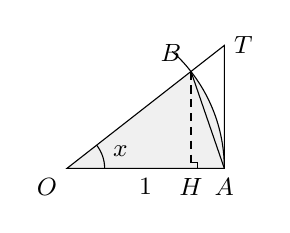
\begin{tikzpicture}[scale=2.0, font=\small]
\coordinate (O) at (0,0);
\coordinate (A) at (1,0);
\coordinate (B) at ({cos(38)},{sin(38)});
\coordinate (T) at (1,{tan(38)});
\coordinate (H) at ({cos(38)},0);
\fill[gray!12] (O)--(A) arc[start angle=0,end angle=38,radius=1]--cycle;
\draw (O)--(A)--(T)--cycle;
\draw (A)--(B);
\draw[densely dashed] (B)--(H);
\draw (H) ++(0,0.04)--++(0.04,0)--++(0,-0.04);
\draw (A) arc[start angle=0,end angle=48,radius=1];
\draw (0.24,0) arc[start angle=0,end angle=38,radius=0.24];
\node at (0.34,0.11) {$x$};
\node[below left] at (O) {$O$};
\node[below] at (A) {$A$};
\node[below] at (H) {$H$};
\node[above left] at (B) {$B$};
\node[right] at (T) {$T$};
\node[below] at (0.5,0) {$1$};
\end{tikzpicture}
\end{center}
作 $BH\perp OA$, 由 $B$ 的坐标有 $BH=\sin x$. 以 $OA=1$ 为底, $\triangle OAB$ 的高为 $BH$, $\triangle OAT$ 的高为 $AT=\tan x$. 单位圆中弧度为 $x$ 的扇形面积为 $\displaystyle\frac x2$. 弦 $AB$ 在圆内, 切线 $AT$ 在圆外, 因而内接三角形严格包含于扇形, 扇形严格包含于外切三角形. 比较面积得
\[
\frac12\sin x<\frac x2<\frac12\tan x,
\qquad\text{即}\quad \sin x<x<\tan x.
\]
结合正弦的奇性, 在零附近有 $|\sin x|\le|x|$. 由夹逼定理, $\displaystyle\lim_{x\to0}\sin x=0$. 当 $\displaystyle|x|\ge\frac\pi2$ 时, 又有 $|\sin x|\le1\le|x|$, 所以这个估计实际上对所有实数都成立. 利用半角公式及刚证的正弦极限,
\[
\begin{aligned}
\lim_{x\to0}(1-\cos x)
&=\lim_{x\to0}2\sin^2\frac x2\\
&=2\left(\lim_{x\to0}\sin\frac x2\right)^2=0.
\end{aligned}
\]
所以 $\displaystyle\lim_{x\to0}\cos x=1$.
\end{cnproof}
任意固定点 $c$ 处的正余弦极限也可由此得到. 令 $h=x-c\to0$, 利用和角公式,
\[
\begin{aligned}
\lim_{h\to0}\sin(c+h)
&=\sin c\lim_{h\to0}\cos h+\cos c\lim_{h\to0}\sin h=\sin c,\\
\lim_{h\to0}\cos(c+h)
&=\cos c\lim_{h\to0}\cos h-\sin c\lim_{h\to0}\sin h=\cos c.
\end{aligned}
\]
\begin{theorem}[第一重要极限]
采用弧度制时, $\displaystyle \lim_{x\to0}\frac{\sin x}{x}=1$.
\end{theorem}
\par\indent\textbf{思路:} $|\sin x|\le|x|$ 只给出了比值的上界, 尚不能说明比值趋于 $1$. 前面的面积比较还给出 $x<\tan x$, 将它改写后便得到一个趋于 $1$ 的下界, 可以使用夹逼.
\begin{cnproof}
对 $\displaystyle0<x<\frac\pi2$, 由已证的 $\sin x<x<\tan x$ 及 $\cos x>0$, 得
\[
\cos x<\frac{\sin x}{x}<1.
\]
因为 $\cos x\to1$, 夹逼给出右极限为 $1$. 比值为偶函数, 左极限也为 $1$, 故双侧极限成立.
\end{cnproof}
\begin{example}
(教材例6.6) 求 $\displaystyle \lim_{x\to0}\frac{1-\cos x}{2x^2}$.
\end{example}
\par\indent\textbf{分析:} $1-\cos x$ 不能直接套 $\displaystyle\frac{\sin t}t$; 用半角公式化成 $\displaystyle2\sin^2\frac x2$, 分母也配成 $(x/2)^2$, 就凑出已知比值. 配分母时要同步保留常数系数, 这是本题最容易漏掉的一步.
\begin{cnproof}
\[
\begin{aligned}
&\lim_{x\to0}\frac{1-\cos x}{2x^2}\\
&\quad=\lim_{x\to0}\frac14\left(\frac{\sin\frac x2}{\frac x2}\right)^2\\
&\quad=\frac14.
\end{aligned}
\]
\end{cnproof}
\begin{example}
(课堂例题: 第一重要极限的基本变形) 求
\[
\text{(1)}\ \lim_{x\to0}\frac{x}{\sin x};\qquad
\text{(2)}\ \lim_{x\to\infty}x\sin\frac1x;\qquad
\text{(3)}\ \lim_{x\to0}\frac{\tan x}{x};\qquad
\text{(4)}\ \lim_{x\to0}\frac{\sin2x}{\tan5x}.
\]
\end{example}
\par\indent\textbf{分析:} 第一题取倒数, 第二题把 $1/x$ 看成趋零变量, 第三题把正切拆成正弦与余弦. 第四题的角不同, 须各自配出“正弦除以同一个角”, 同时保留系数比.
\begin{cnproof}
由第一重要极限与四则法则, 前三题分别为
\[
\begin{aligned}
\lim_{x\to0}\frac{x}{\sin x}&=\frac1{\displaystyle\lim_{x\to0}\frac{\sin x}x}=1,\\
\lim_{x\to\infty}x\sin\frac1x&=\lim_{t\to0}\frac{\sin t}t=1\quad\left(t=\frac1x\right),\\
\lim_{x\to0}\frac{\tan x}x&=\left(\lim_{x\to0}\frac{\sin x}x\right)\frac1{\displaystyle\lim_{x\to0}\cos x}=1.
\end{aligned}
\]
第二题在正、负无穷两个方向都成立. 第四题化为
\[
\begin{aligned}
&\lim_{x\to0}\frac{\sin2x}{\tan5x}\\
&\quad=\lim_{x\to0}\left(\frac25\frac{\sin2x}{2x}\frac{5x}{\sin5x}\cos5x\right)\\
&\quad=\frac25\cdot1\cdot1\cdot1=\frac25.
\end{aligned}
\]
前面的半角例题还给出常用结果 $\displaystyle\frac{1-\cos x}{x^2}\to\frac12$.
\end{cnproof}
\begin{example}
(课堂例题: 反三角函数的换元) 求 $\displaystyle\lim_{x\to0}\frac{\arcsin x}{x}$ 及 $\displaystyle\lim_{x\to0}\frac{\arctan x}{x}$.
\end{example}
\par\indent\textbf{分析:} 已知的是三角函数的基本极限, 而题目出现反函数. 因此把反函数的值记为新变量, 就能把原自变量改写成正弦或正切, 回到上一例. 换元后须先说明新变量确实趋于零.
\begin{cnproof}
令 $t=\arcsin x$, 则 $x=\sin t$. 对任意固定的小角 $\displaystyle0<\eta<\frac\pi2$, 当 $|x|<\sin\eta$ 时, 由正弦在 $[-\pi/2,\pi/2]$ 的单调性可得 $|t|<\eta$, 故 $t\to0$. 去心范围内 $t\ne0$, 因而
\[
\lim_{x\to0}\frac{\arcsin x}x=\lim_{t\to0}\frac t{\sin t}=1.
\]
同理令 $t=\arctan x$, 由 $|x|<\tan\eta$ 得 $|t|<\eta$, 所以 $t\to0$, 并有
\[
\lim_{x\to0}\frac{\arctan x}x=\lim_{t\to0}\frac t{\tan t}=1.
\]
这里用单调性先验证了新变量的趋近过程, 再使用三角函数极限.
\end{cnproof}
\begin{theorem}[第二重要极限]
有
\[
\lim_{x\to\infty}\left(1+\frac1x\right)^x=e,
\qquad
\lim_{t\to0}(1+t)^{\frac1t}=e.
\]
底数在所考察尾部或邻域内为正.
\end{theorem}
\par\indent\textbf{思路:} 数列部分只知道整数下标的结论, 实数 $x$ 不能直接充当那个下标. 因而先用相邻整数 $n=[x]$、$n+1$ 夹住 $x$. 由于倒数随分母增大而减小, 底数被夹在 $\displaystyle1+\frac1{n+1}$ 与 $\displaystyle1+\frac1n$ 之间. 正无穷处这些底数都大于 $1$, 再分别用 $n$ 与 $n+1$ 限制指数, 就得到可由已知数列计算的上下界.

负无穷处不能继续按这一底数大于 $1$ 的方法比较指数. 先令 $y=-x$, 再把底数的倒数写成 $\displaystyle1+\frac1{y-1}$, 就能转回正无穷处已证明的形式.

\begin{cnproof}
先设 $x\to+\infty$, 令 $n=[x]$. 当 $n\ge1$ 时, $n\le x<n+1$, 由底数和指数的单调性,
\[
\left(1+\frac1{n+1}\right)^n
\le\left(1+\frac1x\right)^x
\le\left(1+\frac1n\right)^{n+1}.
\]
两端分别写成 $\displaystyle \frac{(1+\frac1{n+1})^{n+1}}{1+\frac1{n+1}}$ 和 $\displaystyle (1+\frac1n)^n(1+\frac1n)$, 均趋于 $e$, 故夹逼成立. 当 $x\to-\infty$, 令 $y=-x\to+\infty$, 则
\[
\begin{aligned}
&\lim_{y\to+\infty}\left(1-\frac1y\right)^{-y}\\
&\quad=\lim_{y\to+\infty}\left[\left(1+\frac1{y-1}\right)^{y-1}\left(1+\frac1{y-1}\right)\right]\\
&\quad=e\cdot1=e.
\end{aligned}
\]
两个无穷方向同极限. 最后换元 $\displaystyle x=\frac1t$, 得到第二个表达式.
\end{cnproof}
\begin{propositionsingle}[幂指表达式的有限极限]
若 $u(x)\to A$, $v(x)\to B>0$, 则 $v(x)^{u(x)}\to B^A$.
\end{propositionsingle}
\begin{cnproof}
以 $x\to a$ 为例. $v$ 最终为正, 可以写为 $v^u=e^{u\ln v}$. 由已证的对数与指数的点极限,
\[
\begin{aligned}
\lim_{x\to a}v(x)^{u(x)}
&=\lim_{x\to a}\exp\bigl(u(x)\ln v(x)\bigr)\\
&=\exp\left[\left(\lim_{x\to a}u(x)\right)
\ln\left(\lim_{x\to a}v(x)\right)\right]\\
&=e^{A\ln B}=B^A.
\end{aligned}
\]
其他趋近过程同理.
\end{cnproof}
这里指数必须有有限极限. 若指数无界而底数趋于 $1$, 则不能直接代入, 应检查 $u\ln v$ 的极限. 若指数根本没有极限, 原幂指表达式仍可能收敛, 例如底数恒为 $1$.
\par\indent\textbf{幂指极限的转化.} 底数趋于 $1$、指数没有有限极限时, 四则法则不能直接判断结果. 第二重要极限提供了可用的整体 $\displaystyle(1+u)^{\frac1u}$, 因而先将底数写成 $1+u$. 为使指数与已知形式一致, 将原指数 $v$ 写成 $\displaystyle\frac1u$ 的倍数; 这个倍数只能是 $uv$. 于是得到下面的恒等式. 若 $u$ 最终非零、底数最终为正, 且 $uv\to c\in\mathbb R$, 则
\[
(1+u)^v=\left[(1+u)^{\frac1u}\right]^{uv}.
\]
内层底数的极限为 $e>0$, 外层指数的极限为 $c$. 以 $x\to a$ 为例,
\[
\lim_{x\to a}(1+u)^v=\left(\lim_{x\to a}(1+u)^{\frac1u}\right)^{\lim_{x\to a}uv}=e^c.
\]
这里不要求指数本身有极限. 若 $uv$ 不收敛, 则不能由这条有限指数结论直接判断. 取对数也是常用方法, 但 $\ln(1+u)\sim u$ 将在1.8建立, 本节先用重要极限的恒等改写.
\begin{example}
(教材例6.7) 求 $\displaystyle \lim_{x\to\infty}(\frac{2x+1}{2x+3})^x$.
\end{example}
\par\indent\textbf{分析:} 为使用刚得到的转化, 先从底数减去 $1$: 分子与分母的差是 $-2$, 所以增量为 $\displaystyle t=-\frac2{2x+3}$. 原指数 $x$ 与 $\displaystyle1/t$ 不同, 用 $xt$ 补足这个倍数即可. 因而一方面用重要极限控制新的底数, 另一方面计算 $xt$ 是否有有限极限; 两步均成立后才能合并结果.
\begin{cnproof}
令 $\displaystyle t=-\frac2{2x+3}\to0$, 则
\[
\left(\frac{2x+1}{2x+3}\right)^x
=\left[(1+t)^{\frac1t}\right]^{xt},
\qquad \lim_{x\to\infty}xt=\lim_{x\to\infty}\frac{-2x}{2x+3}=-1.
\]
由第二重要极限及有限幂指极限,
\[
\lim_{x\to\infty}\left(\frac{2x+1}{2x+3}\right)^x
=\exp\left(\lim_{x\to\infty}xt\right)=e^{-1}.
\]
此过程同时适用于正、负无穷方向.
\end{cnproof}
\begin{example}
(教材例6.8) 证明 $\displaystyle \lim_{x\to a}x^\mu=a^\mu$, $a>0$, $\mu\in\mathbb R$.
\end{example}
\par\indent\textbf{分析:} 若 $\mu$ 是一般实数, 不能按整数幂作有限次乘法. 对数能把幂函数转为 $e^{\mu\ln x}$, 于是只需依次应用对数与指数的点极限. 条件 $a>0$ 保证 $a$ 附近的 $x$ 也可取对数.
\begin{cnproof}
在 $a$ 的充分小邻域内 $x>0$. 写 $x^\mu=e^{\mu\ln x}$, 由 $\ln x\to\ln a$ 及指数极限, 得 $x^\mu\to e^{\mu\ln a}=a^\mu$.
\end{cnproof}

\subsection{指定作业: 运算与重要极限的应用}
以下题目训练三类转化: 消去导致未定式的公共因子, 将三角式归结为同角比值, 将幂指式归结为第二重要极限. 计算中同时检查定义域与趋近方向.
\begin{example}
(指定作业: 习题1.6第1题(4)) 求 $\displaystyle \lim_{x\to\infty}\frac{x^2-1}{2x^2-x-1}$.
\end{example}
\par\indent\textbf{分析:} 无穷远处的多项式商, 先同除以最高次幂, 使分子分母都有有限极限. 本题分母极限非零, 化简后可直接用商的法则.
\begin{cnproof}
分子分母同除以 $x^2$, 得
\[
\begin{aligned}
&\lim_{x\to\infty}\frac{x^2-1}{2x^2-x-1}\\
&\quad=\lim_{x\to\infty}\frac{1-\frac1{x^2}}{2-\frac1x-\frac1{x^2}}\\
&\quad=\frac12.
\end{aligned}
\]
分母极限为 $2\ne0$, 商的法则可以使用.
\end{cnproof}
\begin{example}
(指定作业: 习题1.6第1题(5)) 求 $\displaystyle \lim_{x\to1}(\frac1{1-x}-\frac3{1-x^3})$.
\end{example}
\par\indent\textbf{分析:} 先看 $1-x^3=(1-x)(1+x+x^2)$, 两分母有共同趋零因子 $1-x$. 通分后, 常数项的抵消又产生 $x-1$, 约去时别漏掉 $1-x=-(x-1)$ 的负号. 这与教材例6.2属于同一种方法.
\begin{cnproof}
两项各自都没有有限极限, 先合并再约分:
\[
\begin{aligned}
&\lim_{x\to1}\left(\frac1{1-x}-\frac3{1-x^3}\right)\\
&\quad=\lim_{x\to1}\frac{x^2+x-2}{(1-x)(1+x+x^2)}\\
&\quad=\lim_{x\to1}\frac{-(x+2)}{1+x+x^2}\\
&\quad=-1.
\end{aligned}
\]
\end{cnproof}
\begin{example}
(指定作业: 习题1.6第1题(6)) 求 $\displaystyle \lim_{x\to4}\frac{\sqrt{2x+1}-3}{\sqrt{x-2}-\sqrt2}$.
\end{example}
\par\indent\textbf{分析:} 直接代入得到两个趋零量之商, 需要比较它们趋零的速度. 每个根式差都可乘共轭式, 变为被开方数之差; 本题这两个差分别为 $2(x-4)$ 和 $x-4$. 这样便显露出共同的趋零因子, 约去后就只剩非零因子的比值.
\begin{cnproof}
在 $4$ 的去心邻域内,
\[
\begin{aligned}
&\lim_{x\to4}\frac{\sqrt{2x+1}-3}{\sqrt{x-2}-\sqrt2}\\
&\quad=\lim_{x\to4}\left[\frac{2(x-4)}{\sqrt{2x+1}+3}\frac{\sqrt{x-2}+\sqrt2}{x-4}\right]\\
&\quad=\lim_{x\to4}\frac{2(\sqrt{x-2}+\sqrt2)}{\sqrt{2x+1}+3}\\
&\quad=\frac{2\sqrt2}3.
\end{aligned}
\]
\end{cnproof}
\begin{example}
(指定作业: 习题1.6第2题(4)) 求 $\displaystyle \lim_{x\to a}\frac{\sin x-\sin a}{x-a}$.
\end{example}
\par\indent\textbf{分析:} 分子是正弦之差, 用和差化积后出现 $\displaystyle\sin\frac{x-a}2$, 它的自变量正好随分母趋零. 将分母配为 $(x-a)/2$, 就能使用第一重要极限; 另一个余弦因子趋于 $\cos a$. 这是“差角除以增量”题型的常用转化.
\begin{cnproof}
由和差化积,
\[
\begin{aligned}
&\lim_{x\to a}\frac{\sin x-\sin a}{x-a}\\
&\quad=\lim_{x\to a}\left(\cos\frac{x+a}{2}\frac{\sin\frac{x-a}{2}}{\frac{x-a}{2}}\right)\\
&\quad=\cos a\cdot1=\cos a.
\end{aligned}
\]
余弦因子的极限使用前面已建立的任意点处三角函数极限.
\end{cnproof}
\begin{example}
(指定作业: 习题1.6第2题(6)) 求 $\displaystyle \lim_{x\to0}\frac{\tan x-\sin x}{\sin^3x}$.
\end{example}
\par\indent\textbf{分析:} 两项各自都趋于零, 不能把差与分母分别取极限. 又因 $\tan x$、$\sin x$ 都与 $x$ 很接近, 简单的大小估计会掩盖相减后的量. 将正切写成 $\displaystyle\frac{\sin x}{\cos x}$ 后通分, 就出现因子 $\sin x(1-\cos x)$. 与分母约去一个正弦后, $\sin^2x$ 可以用平方差公式分解, 因而能够进一步精确约分.
\begin{cnproof}
在零的充分小去心邻域内,
\[
\begin{aligned}
&\lim_{x\to0}\frac{\tan x-\sin x}{\sin^3x}\\
&\quad=\lim_{x\to0}\frac{1-\cos x}{\cos x\sin^2x}\\
&\quad=\lim_{x\to0}\frac1{\cos x(1+\cos x)}\\
&\quad=\frac12.
\end{aligned}
\]
\end{cnproof}
\begin{example}
(指定作业: 习题1.6第2题(8)) 求 $\displaystyle \lim_{x\to0}\frac{\sqrt{1-\cos x}}x$.
\end{example}
\par\indent\textbf{分析:} 开方会使 $\displaystyle\sin\frac x2$ 变成绝对值, 而分母 $x$ 保留正负号. 因此应主动拆成 $|x|/x$ 与趋于正数的因子, 分别计算左右极限. 两侧极限不同足以否定整体极限.
\begin{cnproof}
有
\[
\frac{\sqrt{1-\cos x}}x
=\frac{\sqrt2\,|\sin\frac x2|}{x}
=\frac1{\sqrt2}\frac{|x|}{x}\left|\frac{\sin\frac x2}{\frac x2}\right|.
\]
右极限为 $\displaystyle \frac1{\sqrt2}$, 左极限为 $\displaystyle -\frac1{\sqrt2}$, 故所求双侧极限不存在.
\end{cnproof}
\begin{example}
(指定作业: 习题1.6第2题(10)) 求 $\displaystyle \lim_{x\to0}(1-\tan x)^{\frac1{\sin x}}$.
\end{example}
\par\indent\textbf{分析:} 沿用底数写成 $1+t$ 的办法, 本题 $t=-\tan x$. 外层指数应为原指数与 $t$ 的乘积, 即 $\displaystyle-\frac{\tan x}{\sin x}$, 化简成 $\displaystyle-\frac1{\cos x}$ 后就有有限极限. 负号来自底数中的减号.
\begin{cnproof}
零附近底数为正. 令 $t=-\tan x\to0$, 则
\[
(1-\tan x)^{\frac1{\sin x}}
=\left[(1+t)^{\frac1t}\right]^{-\frac{\tan x}{\sin x}},
\qquad \lim_{x\to0}\frac{-\tan x}{\sin x}=\lim_{x\to0}\frac{-1}{\cos x}=-1.
\]
因此
\[
\lim_{x\to0}(1-\tan x)^{\frac1{\sin x}}
=\exp\left(\lim_{x\to0}\frac{-\tan x}{\sin x}\right)=e^{-1}.
\]
\end{cnproof}
\begin{example}
(指定作业: 习题1.6第2题(11)) 求 $\displaystyle \lim_{x\to\infty}(\frac{2x-1}{2x+1})^x$.
\end{example}
\par\indent\textbf{分析:} 与教材例6.7同型, 将底数写成 $\displaystyle1-\frac2{2x+1}$. 增量与原指数的乘积为 $\displaystyle-\frac{2x}{2x+1}$, 在正、负无穷两个方向都趋于 $-1$, 因而可以统一计算.
\begin{cnproof}
令 $\displaystyle t=-\frac2{2x+1}\to0$, 则底数 $1+t$ 最终为正, 且 $\displaystyle xt=-\frac{2x}{2x+1}\to-1$. 因而
\[
\begin{aligned}
&\lim_{x\to\infty}\left(\frac{2x-1}{2x+1}\right)^x\\
&\quad=\exp\left(\lim_{x\to\infty}\frac{-2x}{2x+1}\right)=e^{-1}.
\end{aligned}
\]
\end{cnproof}
\begin{example}
(指定作业: 习题1.6第2题(13)) 对固定实数 $x$, 求 $\displaystyle \lim_{n\to\infty}(1+\frac xn+\frac{x^2}{2n^2})^{-n}$.
\end{example}
\par\indent\textbf{分析:} 这里趋于无穷的是 $n$, $x$ 是固定参数. 将底数偏离 $1$ 的全部部分记成 $t_n$, 再计算 $-nt_n$. 二次小项乘以 $n$ 后仍趋零, 因此不影响最后的指数, 但不能在恒等变形之前随意删去. 参数 $x=0$ 时 $t_n=0$, 应单独处理以免除以零.
\begin{cnproof}
若 $x=0$, 数列恒为 $1$. 若 $x\ne0$, 令 $\displaystyle t_n=\frac xn+\frac{x^2}{2n^2}$. 则 $t_n\to0$, 且充分大的 $n$ 有 $t_n\ne0$. 又底数 $\displaystyle 1+t_n=\frac12[(1+\frac xn)^2+1]>0$. 于是
\[
(1+t_n)^{-n}
=\left[(1+t_n)^{\frac1{t_n}}\right]^{-nt_n},
\qquad \lim_{n\to\infty}(-nt_n)=\lim_{n\to\infty}\left(-x-\frac{x^2}{2n}\right)=-x.
\]
由重要极限及海涅定理, 方括号内趋于 $e$, 所以
\[
\lim_{n\to\infty}\left(1+\frac xn+\frac{x^2}{2n^2}\right)^{-n}
=\exp\left(\lim_{n\to\infty}(-nt_n)\right)=e^{-x}.
\]
\end{cnproof}
\begin{example}
(指定作业: 习题1.6第2题(14)) 求 $\displaystyle \lim_{x\to0}(\cos x)^{\frac1{x^2}}$.
\end{example}
\par\indent\textbf{分析:} 按幂指式的转化, 取底数相对 $1$ 的增量 $t=\cos x-1$, 需要计算它与原指数的乘积 $\displaystyle t/x^2$. 这正是前面用半角公式求过的余弦二阶比值, 极限为 $\displaystyle-\frac12$. 底数趋于 $1$ 本身不足以判断结果, 增量与指数的乘积才给出所需的有限指数.
\begin{cnproof}
令 $t=\cos x-1\to0$, 则零的充分小去心邻域内 $t\ne0$, 且
\[
\begin{aligned}
&\lim_{x\to0}\frac{t}{x^2}\\
&\quad=\lim_{x\to0}\frac{-(1-\cos x)}{x^2}\\
&\quad=-\frac12.
\end{aligned}
\]
故
\[
\begin{aligned}
&\lim_{x\to0}(\cos x)^{\frac1{x^2}}\\
&\quad=\exp\left(\lim_{x\to0}\frac{t}{x^2}\right)=e^{-\frac12}.
\end{aligned}
\]
\end{cnproof}
\begin{example}
(指定作业: 习题1.6第6题) 已知 $\displaystyle \lim_{x\to\infty}(\frac{x+a}{x-a})^x=9$, 求常数 $a$.
\end{example}
\par\indent\textbf{分析:} 这是把幂指极限反过来用于求参. 先保留 $a$ 算出一般极限, 再令它等于 $9$. 底数减去 $1$ 后为 $2a/(x-a)$, 与指数相乘趋于 $2a$. $a=0$ 时不能用含 $1/t$ 的改写, 先直接检查.
\begin{cnproof}
$a=0$ 时极限为 $1$, 不合题意. 当 $a\ne0$ 时, 令 $\displaystyle t=\frac{2a}{x-a}\to0$, 则
\[
\left(\frac{x+a}{x-a}\right)^x
=\left[(1+t)^{\frac1t}\right]^{xt},
\qquad \lim_{x\to\infty}xt=\lim_{x\to\infty}\frac{2ax}{x-a}=2a.
\]
于是两个无穷方向都有
\[
\lim_{x\to\infty}\left(\frac{x+a}{x-a}\right)^x
=\exp\left(\lim_{x\to\infty}xt\right)=e^{2a}.
\]
由 $e^{2a}=9$, 得 $\displaystyle a=\frac12\ln9=\ln3$.
\end{cnproof}

\section{无穷小和无穷大}
前面用极限计算函数的趋近值. 本节进一步比较趋近的速度: 两个量都趋于零时, 它们的商可能趋零、趋于非零常数, 也可能没有有限极限. 这种比较能识别表达式的主要部分, 但必须先明确所考察的极限过程.
\subsection{无穷小及其运算}
\begin{definition}
在指定极限过程中, 以 $0$ 为极限的变量称为\textbf{无穷小量}, 简称\textbf{无穷小}. 讨论时必须指明极限过程.
\end{definition}
非零常数无论数值多小, 都不是无穷小; 恒为零的量则符合定义. 同一个表达式在不同过程中性质可能不同, 例如 $x$ 在 $x\to0$ 时为无穷小, 在 $x\to+\infty$ 时则不是. 写 $f=L+\alpha$ 的意义, 是将函数分成确定的极限值与趋于零的误差.
\begin{example}
(教材例7.1) 说明 $(x-a)^2$、$\sin(x-a)$ 在 $x\to a$ 时, 以及 $\displaystyle \frac1x$、$\displaystyle \frac1{3x}$、$\displaystyle \frac{x^2+x+1}{x^3+2}$ 在 $x\to\infty$ 时均为无穷小.
\end{example}
\par\indent\textbf{分析:} 判断无穷小, 只需检查指定过程中的极限是否为零. 前四个式子可直接用已有极限; 最后一个是多项式商, 在无穷远处应提取最高次幂, 看分子、分母还剩什么. 不必重新逐个写误差定义.
\begin{cnproof}
前两者由幂函数与正弦在零点的极限得零; 中间两者是 $\displaystyle \frac1x$ 的常数倍; 最后一项分子分母同除以 $x^3$, 得
\[
\begin{aligned}
&\lim_{x\to\infty}\frac{x^2+x+1}{x^3+2}\\
&\quad=\lim_{x\to\infty}\frac{\frac1x+\frac1{x^2}+\frac1{x^3}}{1+\frac2{x^3}}\\
&\quad=0.
\end{aligned}
\]
\end{cnproof}
\begin{theoremsingle}
$f(x)\to L$ 等价于 $f(x)=L+\alpha(x)$, 其中 $\alpha$ 为同一过程中的无穷小.
\end{theoremsingle}
\begin{cnproof}
若 $f\to L$, 令 $\alpha=f-L$, 则 $\alpha\to0$. 反过来, $f=L+\alpha$ 且 $\alpha\to0$ 时由和的法则得 $f\to L$.
\end{cnproof}
\begin{proposition}
有限个无穷小的和仍为无穷小; 无穷小与局部有界变量的乘积为无穷小. 特别地, 有限个无穷小的乘积仍为无穷小.
\end{proposition}
\begin{cnproof}
有限和由四则运算法则得出. 若 $|\beta|\le M$, $M>0$, 而 $\alpha\to0$, 则任给 $\varepsilon>0$, 使 $\displaystyle |\alpha|<\frac\varepsilon M$ 后便有 $|\alpha\beta|<\varepsilon$. 无穷小本身局部有界, 故乘积结论随之得到.
\end{cnproof}
无穷多个无穷小的和不一定仍趋于零, 项数随变量增多时尤其不能直接套用有限和的法则. 无穷小的商也没有统一结论, 例如 $\displaystyle \frac{x^2}{x}\to0$, $\displaystyle \frac xx=1$, $\displaystyle \frac x{x^2}$ 则没有有限极限.
\subsection{无穷大及其与无穷小的联系}
\begin{definition}
以 $x\to a$ 为例. 若任给 $M>0$, 都存在 $\delta>0$, 使 $0<|x-a|<\delta$ 时恒有 $|f(x)|>M$, 则称 $f$ 为\textbf{无穷大量}, 记 $f(x)\to\infty$. 若将最后的条件换为 $f(x)>M$ 或 $f(x)<-M$, 则分别称\textbf{正无穷大}或\textbf{负无穷大}. 在其他极限过程中, 将去心邻域换为相应的单侧范围或无穷尾部.
\end{definition}
这里 $\infty$ 不表示某个实数, $f\to\infty$ 表示绝对值在整个趋近范围内最终超过任给正数, 并不要求最终同号. 例如 $\displaystyle\frac1x$ 在 $x\to0$ 时为无穷大, 但左右符号不同. 无界仅保证能找到任意大的绝对值, 不能保证其余充分靠近的点也如此; 后面的 $x\cos x$ 将说明两者的区别.
\begin{example}
(教材例7.2) 用定义证明 $\displaystyle \frac{x+2}{x^2-1}\to\infty$, $x\to1$.
\end{example}
\par\indent\textbf{分析:} 按定义应使原式的绝对值大于任意给定的 $M$. 分母趋零还不够, 因为分子可能同时趋零并抵消这种增长. 将分母分解为 $(x-1)(x+1)$, 可把绝对值写成 $\displaystyle\left|\frac{x+2}{x+1}\right|\frac1{|x-1|}$. 后一个因子会因 $x\to1$ 增大, 前一个因子则要保证不接近零.

在 $1$ 的一个固定邻域内, $\displaystyle\frac{x+2}{x+1}=1+\frac1{x+1}>1$. 因而整体大于 $\displaystyle\frac1{|x-1|}$. 到此再反解 $\displaystyle\frac1{|x-1|}>M$, 就能选出所需半径. 这里先作下界估计, 再按任给的 $M$ 缩小邻域.
\begin{cnproof}
先限制 $\displaystyle0<|x-1|<\frac12$, 则 $\displaystyle\frac12<x<\frac32$. 此时 $x+1>0$, 且
\[
\frac{x+2}{x+1}=1+\frac1{x+1}>1.
\]
因此
\[
\left|\frac{x+2}{x^2-1}\right|=\frac{x+2}{x+1}\frac1{|x-1|}>\frac1{|x-1|}.
\]
任给 $M>0$, 取 $\displaystyle\delta=\min\left\{\frac12,\frac1M\right\}$. 当 $0<|x-1|<\delta$ 时, 既满足上述估计的范围, 又有 $\displaystyle\frac1{|x-1|}>M$, 从而原式的绝对值大于 $M$. 这就满足无穷大的定义.

在所限范围内, 因子 $\displaystyle\frac{x+2}{x+1}$ 为正, 故原式的符号由 $x-1$ 决定: 左侧趋于负无穷, 右侧趋于正无穷. 所以这里写 $\infty$ 表示绝对值无限增大, 不能写成两侧都趋于 $+\infty$.
\end{cnproof}
\begin{proposition}
若 $\alpha\to0$ 且在所考察范围内非零, 则 $\displaystyle \frac1\alpha\to\infty$; 若 $f\to\infty$, 则 $\displaystyle \frac1f\to0$. 两个无穷大的乘积为无穷大; 无穷大与局部有界变量的和仍为无穷大.
\end{proposition}
\begin{cnproof}
倒数结论分别用阈值 $M$ 与误差 $\displaystyle \frac1M$ 相互转换. 对乘积, 使两个因子的绝对值都大于 $\sqrt M$, 则积大于 $M$. 对和, 若 $|g|\le C$, 则使 $|f|>M+C$, 由反三角不等式有 $|f+g|\ge|f|-|g|>M$.
\end{cnproof}
无穷大之和可能相互抵消, 无穷大与无穷小的乘积也需单独分析. 例如 $x\to+\infty$ 时, $\displaystyle x\cdot\frac1{x^2}\to0$, $\displaystyle x\cdot\frac1x=1$, $\displaystyle x\cdot\frac1{\sqrt x}\to+\infty$.
\subsection{无穷小的阶、等价与主部}
两个无穷小之差总趋于零, 不能用它判断两者大小是否接近. 例如 $x$ 与 $x^2$ 的差趋零, $x$ 与 $2x$ 的差也趋零, 但它们的相对大小不同. 因而改看比值: 以其中一个量作为尺度, 比较另一个量占它的多少.
\begin{definition}
设同一极限过程中 $\alpha,\beta\to0$, 且 $\beta$ 最终非零. 若 $\displaystyle \frac\alpha\beta\to k\ne0$, 称它们为\textbf{同阶无穷小}; 若该比值趋于 $1$, 称为\textbf{等价无穷小}, 记 $\alpha\sim\beta$; 若比值趋于 $0$, 称 $\alpha$ 为比 $\beta$ \textbf{高阶的无穷小}, 记 $\alpha=o(\beta)$. 若 $\displaystyle\left|\frac\alpha\beta\right|\to+\infty$, 则称 $\alpha$ 为比 $\beta$ \textbf{低阶的无穷小}.
\end{definition}
教材将有限非零比值的同阶关系记为 $O(\beta)$. 通常文献中的大 $O$ 还可表示更宽的“比值有界”关系; 为避免混淆, 本稿同阶判断直接列出比值的非零极限. 只出现 $o$ 时, 均按上述比值趋零的意义使用.
\begin{definition}
当 $x\to0^+$ 时, 若 $\displaystyle \frac{\alpha(x)}{x^\mu}\to k\ne0$, $\mu>0$, 则称 $\alpha$ 为关于 $x$ 的\textbf{$\mu$ 阶无穷小}, $kx^\mu$ 为相应\textbf{主部}. 对两侧极限, 须另行保证实数幂在所考察两侧有定义; 整数阶通常没有这一障碍.
\end{definition}
比较之前要先认准标准量和极限过程. 高阶无穷小表示“比标准量更快趋于零”, 例如 $x^2=o(x)$; 同阶只说明比值趋于非零常数, 等价还要求这个常数恰为 $1$. 例如 $2x$ 与 $x$ 同阶, 却不等价. 若不满足上述任何一种比值条件, 就不能强行判为其中一类.

阶数越高表示相对标准量衰减得越快. 主部中的系数允许为负, 因而它同时保留大小与符号信息. 例如主部为 $-2x^3$ 的意思是原量除以 $x^3$ 趋于 $-2$, 不只说明其绝对值与 $x^3$ 同阶.
\begin{proposition}
$\alpha\sim\beta$ 等价于 $\alpha=\beta+o(\beta)$. 等价关系具有对称性和传递性. 若 $\alpha\sim\widetilde\alpha$, $\beta\sim\widetilde\beta$, 则商的极限可以用对应等价量替换, 只要所涉及商在最终范围内有意义.
\end{proposition}
\begin{cnproof}
将 $\alpha$ 与 $\beta$ 的差按 $\beta$ 的尺度衡量, 有
\[
\frac{\alpha-\beta}{\beta}=\frac\alpha\beta-1.
\]
因此 $\alpha/\beta\to1$ 等价于 $\alpha-\beta=o(\beta)$. 比值趋于 $1$ 还保证 $\alpha$ 最终非零, 取倒数得对称性. 若另有 $\beta\sim\gamma$, 则由 $\displaystyle\frac\alpha\gamma=\frac\alpha\beta\frac\beta\gamma\to1$ 得传递性. 商的替换利用
\[
\frac\alpha\beta
=\frac\alpha{\widetilde\alpha}\cdot
\frac{\widetilde\alpha}{\widetilde\beta}\cdot
\frac{\widetilde\beta}{\beta}.
\]
两端比值趋于 $1$, 中间若有有限或无穷极限, 则左右同极限. 无穷情形由绝对值最终与正的常数倍夹住来证明.
\end{cnproof}
\par\indent\textbf{使用要点:} 商的替换公式把原商写成替换后的商乘上两个趋于 $1$ 的因子, 所以有限或无穷极限都不改变. 这种乘法关系不直接适用于差: 若两个主部抵消, 结果的尺度会变小, 原先可忽略的误差便可能决定结果.

等价替换优先用于乘积和商. 和差中的主项可能抵消, 不能把每一项分别替换后就丢掉误差. 例如 $\tan x\sim x$, $\sin x\sim x$, 却不能以 $x-x=0$ 计算 $\tan x-\sin x$ 的主部.
\begin{example}
(教材例7.3) 求 $\displaystyle \lim_{x\to0}\frac{x(\tan x-\sin x)}{\sin x^4}$, 其中分母是 $\sin(x^4)$.
\end{example}
\par\indent\textbf{分析:} 分子中的两个三角函数都以 $x$ 为一阶主部, 相减会抵消, 所以不能分别替换. 看到 $\tan x-\sin x$, 先把正切写成正弦除以余弦, 就能提出 $\sin x$, 将差化为乘积. 乘积中的 $\sin x$、$1-\cos x$ 和 $\cos x$ 都已有熟悉的极限或等价量, 此时才适合替换.
\begin{cnproof}
在零的充分小去心邻域内, $\cos x\ne0$. 先作恒等变形:
\[
\tan x-\sin x=\frac{\sin x}{\cos x}-\sin x
=\frac{\sin x(1-\cos x)}{\cos x}.
\]
于是
\[
\frac{x(\tan x-\sin x)}{\sin(x^4)}
=\frac{\sin x}{x}\cdot\frac{1-\cos x}{x^2}
 \cdot\frac1{\cos x}\cdot\frac{x^4}{\sin(x^4)}.
\]
因此应用乘积极限法则,
\[
\begin{aligned}
&\lim_{x\to0}\frac{x(\tan x-\sin x)}{\sin(x^4)}\\
&\quad=\left(\lim_{x\to0}\frac{\sin x}x\right)
\left(\lim_{x\to0}\frac{1-\cos x}{x^2}\right)
\left(\lim_{x\to0}\frac1{\cos x}\right)
\left(\lim_{x\to0}\frac{x^4}{\sin(x^4)}\right)\\
&\quad=1\cdot\frac12\cdot1\cdot1=\frac12.
\end{aligned}
\]
精确分解先保留了相减后的部分, 随后才能分别计算各因子的极限.
\end{cnproof}
\begin{example}
(教材例7.4) 当 $x\to0$ 时, $\sqrt{1+x^2}-\sqrt{1-x^2}$ 为 $x$ 的几阶无穷小?
\end{example}
\par\indent\textbf{分析:} 两个根式都趋于 $1$, 各自的极限不能反映相减后余下的大小. 根式差适合有理化, 因为 $(\sqrt A-\sqrt B)(\sqrt A+\sqrt B)=A-B$, 能把抵消后的部分精确显露出来. 本题有理化后分子为 $2x^2$, 分母趋于 $2$, 因而自然选 $x^2$ 作比较尺度. 还要验证比值的极限非零, 才能断定恰为二阶.
\begin{cnproof}
有
\[
\begin{aligned}
&\lim_{x\to0}\frac{\sqrt{1+x^2}-\sqrt{1-x^2}}{x^2}\\
&\quad=\lim_{x\to0}\frac2{\sqrt{1+x^2}+\sqrt{1-x^2}}\\
&\quad=1.
\end{aligned}
\]
故为二阶无穷小, 且等价于 $x^2$.
\end{cnproof}
\begin{example}
(教材例7.5) 在 $x\to+\infty$ 时, 写出 $\displaystyle \frac1{x\sqrt{1+x^2}}$ 的主部和余项形式.
\end{example}
\par\indent\textbf{分析:} 在 $x\to+\infty$ 时, $\sqrt{1+x^2}$ 的主要大小与 $x$ 相同, 所以原分母的主要大小为 $x^2$, 提示主部应为 $\displaystyle\frac1{x^2}$. 猜到主部后仍须用比值趋于 $1$ 验证, 才能写余项为小 $o$. 提取根号内的平方因子时, 必须记住 $\sqrt{x^2}=|x|$; 本题因 $x$ 最终为正才能写成 $x$.
\begin{cnproof}
\[
\begin{aligned}
&\lim_{x\to+\infty}\frac{\frac1{x\sqrt{1+x^2}}}{\frac1{x^2}}\\
&\quad=\lim_{x\to+\infty}\frac1{\sqrt{1+\frac1{x^2}}}\\
&\quad=1.
\end{aligned}
\]
故主部为 $\displaystyle \frac1{x^2}$, 并有 $\displaystyle \frac1{x\sqrt{1+x^2}}=\frac1{x^2}+o(\frac1{x^2})$. 必须保留 $x\to+\infty$ 的方向; 在负无穷方向原式为负, 主部应为 $\displaystyle -\frac1{x^2}$.
\end{cnproof}
\par\indent\textbf{无穷大的比较.} 比较无穷大同样先作比值. 对同一过程中的无穷大 $F,G$, 若 $F/G$ 趋于有限非零常数, 称它们同阶; 趋于 $1$ 时称等价. 若 $F/G\to0$, 则 $F$ 比 $G$ 增长得慢; 若 $|F/G|\to+\infty$, 则增长得快.

若 $\displaystyle\frac F{G^\mu}\to k\ne0$, $\mu>0$, 则称 $F$ 是关于标准无穷大量 $G$ 的 $\mu$ 阶无穷大, 主部为 $kG^\mu$. 使用非整数幂时须保证相应实数幂有定义. 小 $o$ 仍表示比值趋零: $R=o(G)$ 并不要求余项 $R$ 自身趋零.

\begin{example}
(教材例7.6) 当 $x\to1$ 时, 求 $\displaystyle \frac1{\sin\pi x}$ 关于 $\displaystyle \frac1{x-1}$ 的阶与主部.
\end{example}
\par\indent\textbf{分析:} 已知等价量 $\sin t\sim t$ 的条件是 $t\to0$, 本题 $\pi x\to\pi$, 不能直接套用. 先令 $h=x-1$, 将趋近点平移到零, 再用三角恒等式处理 $\sin(\pi+\pi h)$. 这样不仅得到阶数, 也能保留主部的负号.
\begin{cnproof}
令 $h=x-1$, 则 $h\to0$, 且
\[
\sin\pi x=\sin(\pi+\pi h)=-\sin\pi h.
\]
用给定的标准量作除数, 得
\[
\begin{aligned}
&\lim_{x\to1}\frac{\frac1{\sin\pi x}}{\frac1{x-1}}\\
&\quad=\lim_{x\to1}\frac{x-1}{\sin\pi x}\\
&\quad=-\frac1\pi\lim_{h\to0}\frac{\pi h}{\sin\pi h}=-\frac1\pi.
\end{aligned}
\]
比值的极限有限且非零, 故两者为同阶无穷大, 相对于标准量 $\displaystyle\frac1{x-1}$ 为一阶, 主部为 $\displaystyle-\frac1{\pi(x-1)}$. 因而也可写为
\[
\frac1{\sin\pi x}=-\frac1{\pi(x-1)}+o\!\left(\frac1{x-1}\right).
\]
这里的小 $o$ 仍表示余项除以括号内标准量趋于零, 并不表示余项本身必为无穷小.
\end{cnproof}
\begin{example}
(教材例7.7) 已知 $\displaystyle \lim_{x\to\infty}(\frac{x^2}{x+1}-ax-b)=0$, 求 $a,b$.
\end{example}
\par\indent\textbf{分析:} 这里要求的是原函数与直线之差趋零, 只找等价的一次项还不够, 因为相差一个非零常数也不符合要求. 分子次数比分母高一次, 多项式除法能够依次提取一次项和常数项, 剩下的真分式趋零. 这恰好对应所求的 $ax+b$, 因而先作精确除法, 再分别消去增长项和常数项.
\begin{cnproof}
\[
\frac{x^2}{x+1}=x-1+\frac1{x+1},
\qquad
\frac{x^2}{x+1}-ax-b=(1-a)x-(1+b)+\frac1{x+1}.
\]
若 $a\ne1$, 线性项无界, 不可能与有界的其余部分合成趋零量, 故 $a=1$. 再由极限为零得 $-(1+b)=0$, 即 $b=-1$. 代回余项为 $\displaystyle \frac1{x+1}\to0$, 验证成立.
\end{cnproof}
\begin{example}
(选自教材习题1.7第6题) 为什么不能把 $\displaystyle \frac{\tan x-\sin x}{x^3}$ 中的两个三角函数分别替换为 $x$?
\end{example}
\par\indent\textbf{分析:} 等价替换省略的是相对于原量更小的误差. 但主部相减后, 原先较小的误差可能成为结果的主要部分. 本题与教材例7.3是同一结构, 直接沿用其中的因式分解即可.

\begin{cnproof}
两项分别替换会丢掉相减后留下的部分. 由教材例7.3中的精确分解得到 $\displaystyle \tan x-\sin x\sim\frac{x^3}{2}$, 故商极限为 $\displaystyle \frac12$, 而不是 $0$.
\end{cnproof}
对多项式商, $x\to0$ 时比较最低非零次项, $|x|\to\infty$ 时比较最高次项. 这一规则是提取主部后的商替换, 并不依赖求导.

\begin{example}
(补充题型: 主项抵消与求参) 求 $a$, 使 $\sqrt{1+x}-1-ax$ 在 $x\to0$ 时是关于 $x$ 的二阶无穷小, 并写出主部.
\end{example}
\par\indent\textbf{分析:} 设所求表达式为 $R(x)$. 若它是二阶无穷小, 则 $\displaystyle\frac{R(x)}{x^2}$ 应趋于非零常数, 从而 $\displaystyle\frac{R(x)}x=x\frac{R(x)}{x^2}\to0$. 后一个必要条件更容易处理: 根式有理化后, $\displaystyle\frac{R(x)}x$ 的极限只含参数 $a$, 可以先据此确定候选值. 再对这个值计算 $\displaystyle\frac{R(x)}{x^2}$, 检查抵消后留下的是二阶量, 还是更高阶量.
\begin{cnproof}
若原式为二阶量, 则它除以 $x$ 的比值必须趋零. 而
\[
\begin{aligned}
&\lim_{x\to0}\frac{\sqrt{1+x}-1-ax}{x}\\
&\quad=\lim_{x\to0}\left(\frac1{\sqrt{1+x}+1}-a\right)\\
&\quad=\frac12-a.
\end{aligned}
\]
所以必须 $\displaystyle a=\frac12$. 对此取值, 再有理化得
\[
\sqrt{1+x}-1-\frac x2
=\frac{x(1-\sqrt{1+x})}{2(\sqrt{1+x}+1)}
=-\frac{x^2}{2(\sqrt{1+x}+1)^2}.
\]
所以
\[
\lim_{x\to0}\frac{\sqrt{1+x}-1-\frac x2}{x^2}
=\lim_{x\to0}\frac{-1}{2(\sqrt{1+x}+1)^2}=-\frac18\ne0.
\]
故恰为二阶, 主部为 $\displaystyle-\frac{x^2}8$.
\end{cnproof}
\subsection{指定作业与典型题型}
\begin{example}
(指定作业: 习题1.7第3题) $f(x)=x\cos x$ 在实数轴上是否有界? 当 $x\to\infty$ 时是否为无穷大?
\end{example}
\par\indent\textbf{分析:} 无界只需找到任意大的取值; 无穷大却要求所有充分远处的绝对值都大. 因此分别寻找波峰点和零点, 就能区分这两个判断.
\begin{cnproof}
取 $x_n=2n\pi$, 则 $f(x_n)=2n\pi\to+\infty$, 故无界. 但取 $\displaystyle y_n=\frac\pi2+n\pi$, 则 $y_n\to+\infty$ 且 $f(y_n)=0$. 无论阈值取得多远, 仍有这样的零点, 因而不满足无穷大的定义. 所以它无界, 却不是无穷大.
\end{cnproof}
\begin{example}
(指定作业: 习题1.7第5题(2)(4)) 证明
\[
\frac{x+2}{x^4+3}=o\!\left(\frac1{x^2}\right)\quad(x\to\infty),
\qquad
\sqrt{x+1}-\sqrt x=O\!\left(\frac1{\sqrt x}\right)\quad(x\to+\infty).
\]
第二式按老师更正取正无穷方向; 此处 $O$ 沿用教材表示同阶的约定.
\end{example}
\par\indent\textbf{分析:} 验证阶的关系, 先作“待比较量除以标准量”的比值. 比值趋零对应小 $o$, 趋于有限非零常数对应教材所说的同阶. 根式差仍先有理化.
\begin{cnproof}
第一式的比值为
\[
\begin{aligned}
&\lim_{x\to\infty}\frac{\frac{x+2}{x^4+3}}{\frac1{x^2}}\\
&\quad=\lim_{x\to\infty}\frac{\frac1x+\frac2{x^2}}{1+\frac3{x^4}}\\
&\quad=0.
\end{aligned}
\]
第二式的比值为
\[
\begin{aligned}
&\lim_{x\to+\infty}\frac{\sqrt{x+1}-\sqrt x}{\frac1{\sqrt x}}\\
&\quad=\lim_{x\to+\infty}\frac1{\sqrt{1+\frac1x}+1}\\
&\quad=\frac12.
\end{aligned}
\]
故两式成立. 第二式还给出更精确的等价量 $\displaystyle\sqrt{x+1}-\sqrt x\sim\frac1{2\sqrt x}$.
\end{cnproof}
\begin{example}
(指定作业: 习题1.7第7题(4)) 当 $x\to0$ 时, 求 $\tan x-\sin x$ 的阶及主部. 并计算 $\displaystyle\lim_{x\to0}\frac{\tan x-\sin x}{x^2}$, 比较分母为 $x^3$ 的情形.
\end{example}
\begin{cnproof}
前面已将差化为 $\displaystyle\frac{\sin x(1-\cos x)}{\cos x}$, 因而
\[
\begin{aligned}
&\lim_{x\to0}\frac{\tan x-\sin x}{x^3}\\
&\quad=\lim_{x\to0}\left(\frac{\sin x}{x}\frac{1-\cos x}{x^2}\frac1{\cos x}\right)\\
&\quad=1\cdot\frac12\cdot1=\frac12.
\end{aligned}
\]
所以它是三阶无穷小, 主部为 $\displaystyle\frac{x^3}{2}$. 同一变形既能求商的极限, 也能确定阶和主部.

分母改为 $x^2$ 时, 将已求得的比值乘以 $x$, 得
\[
\begin{aligned}
&\lim_{x\to0}\frac{\tan x-\sin x}{x^2}\\
&\quad=\lim_{x\to0}\left(x\frac{\tan x-\sin x}{x^3}\right)\\
&\quad=0\cdot\frac12=0.
\end{aligned}
\]
所以分母为 $x^2$、$x^3$ 时的结果分别为 $0$、$\displaystyle\frac12$. 这两问分别比较同一个三阶量与不同的尺度, 无需重复寻找变形.
\end{cnproof}
\begin{example}
(指定作业: 习题1.7第8题(4)) 求
\[
\lim_{x\to0^+}\frac{\sin(x^3)\tan x(1-\cos x)}{\sqrt{x+\sqrt[3]x}\,\sqrt[6]{x^5}\sin^5x}.
\]
\end{example}
\par\indent\textbf{分析:} 三角因子都已处于小变量范围, 可以用基本等价量比较幂次. 需要先处理的是根号内的和: 若直接分别对 $x$ 与 $\sqrt[3]x$ 取主部, 还不知道谁决定总和的大小. 将两者作比值得 $\displaystyle\frac{x}{\sqrt[3]x}=x^{\frac23}\to0$, 所以应提出较大的 $x^{\frac13}$. 剩下的因子趋于 $1$, 才能确定整个根式的尺度. 最后将乘商中各因子的幂次与系数分别合并.
\begin{cnproof}
有
\[
\sqrt{x+\sqrt[3]x}=x^{\frac16}\sqrt{1+x^{\frac23}}\sim x^{\frac16},
\qquad\sqrt[6]{x^5}=x^{\frac56}.
\]
分子主部为 $\displaystyle x^3\cdot x\cdot\frac{x^2}2=\frac{x^6}2$, 分母主部为 $\displaystyle x^{\frac16}x^{\frac56}x^5=x^6$, 据等价替换定理,
\[
\lim_{x\to0^+}\frac{\sin(x^3)\tan x(1-\cos x)}{\sqrt{x+\sqrt[3]x}\,\sqrt[6]{x^5}\sin^5x}
=\lim_{x\to0^+}\frac{x^6}{2x^6}=\frac12.
\]
原题的 $\sin(x^3)$ 指先立方再取正弦.
\end{cnproof}

\section{连续函数}
函数极限只考察一个点附近的变化, 不要求该点本身有函数值. 若还要使附近的函数值趋近于该点的实际函数值, 就得到连续性. 本节先区分这两个要求, 再利用连续性将已知极限传递给复合函数, 建立对数、指数与幂函数的基本等价量.
\subsection{连续的定义与间断点}
\begin{definition}
设 $f$ 在 $x_0$ 的一个邻域内有定义. 若任给 $\varepsilon>0$, 存在 $\delta>0$, 使 $|x-x_0|<\delta$ 时 $|f(x)-f(x_0)|<\varepsilon$, 则称 $f$ 在 $x_0$ \textbf{连续}. 在区间每点都连续的函数称该区间上的\textbf{连续函数}.
\end{definition}
连续要求中心点有函数值, 并要求周围函数值趋于这一中心值. 因而连续等价于三个条件同时满足: $f(x_0)$ 有定义, $\displaystyle \lim_{x\to x_0}f(x)$ 存在, 且二者相等. 令 $\Delta x=x-x_0$, $\Delta y=f(x_0+\Delta x)-f(x_0)$, 也可表述为 $\Delta x\to0$ 时 $\Delta y\to0$.
在闭区间 $[a,b]$ 上连续, 指内部每点连续, 并在 $a$ 处右连续、在 $b$ 处左连续. 记全体这样的函数为 $C[a,b]$. 端点只考察区间内的趋近方向.
\begin{definition}
设 $f$ 在 $x_0$ 的某个去心邻域内有定义. 若 $f(x_0)$ 无定义, 或虽有定义但在 $x_0$ 不连续, 则称 $x_0$ 为\textbf{间断点}. 两个单侧有限极限均存在时称为\textbf{第一类间断点}; 否则称为\textbf{第二类间断点}. 第一类中, 若两个极限相等, 称为\textbf{可去间断点}; 若不等, 称为\textbf{跳跃间断点}.
\end{definition}
上述定义沿用教材的约定, 将没有中心值但两侧有定义的情形也纳入讨论. 分类依据先是两侧的变化, 再是中心值: 两个单侧极限共同为 $L$ 时, 补充或改取 $f(x_0)=L$ 就能连续; 两侧没有共同有限极限时, 只改中心值不能消除间断. 端点处的连续性仍按相应单侧定义判断.
\begin{example}
(教材例8.1) 比较以下函数在 $0$ 处的连续性:
\[
f_1(x)=x^2,\quad
f_2(x)=\begin{cases}|x|,&x\ne0,\\2,&x=0,\end{cases}\quad
f_3(x)=\frac{\sin x}{x}\ (x\ne0),\quad
f_4(x)=\begin{cases}e^{\frac1x},&x\ne0,\\1,&x=0.\end{cases}
\]
\end{example}
\par\indent\textbf{分析:} 依次检查“中心值有无定义、左右极限是否相等、极限是否等于中心值”. 前三个函数分别展示连续、中心值取错和中心值缺失; 最后一个要看左右两侧, 单独调整中心值无法修复两侧的差异.
\begin{cnproof}
$f_1$ 的极限等于中心值 $0$, 故连续. $f_2$ 的极限为 $0$, 却有中心值 $2$, 因而为可去间断; 改 $f_2(0)=0$ 即可. $f_3$ 在 $0$ 未定义, 但极限为 $1$, 补 $f_3(0)=1$ 后连续. $f_4$ 左极限为 $0$, 右侧无界增大, 所以为第二类间断, 改中心值不能使它连续.
\end{cnproof}
取整函数 $[x]$ 在每个整数处为跳跃间断, 右、左极限之差为 $1$. 判断间断时, 应先算两个单侧极限, 再比较中心值.
\begin{example}
(教材例8.2) 设
\[
f(x)=\begin{cases}\frac{\sin x}{x},&x<0,\\a,&x=0,\\x\sin\frac1x+b,&x>0.\end{cases}
\]
分别求 $0$ 处极限存在、连续的参数条件.
\end{example}
\par\indent\textbf{分析:} 分段点处, 左、右极限要分别按对应表达式计算. $\sin(1/x)$ 自身不趋于固定值, 但它有界, 乘上趋零的 $x$ 后可以用夹逼法处理. 极限存在只约束左右两侧, 连续则还要约束中间参数 $a$.
\begin{cnproof}
左极限为 $1$. 右侧 $\displaystyle |x\sin\frac1x|\le|x|\to0$, 所以右极限为 $b$. 双侧极限存在当且仅当 $b=1$, 此时 $a$ 可任取. 若还要求连续, 必须中心值与极限相等, 故 $a=b=1$.
\end{cnproof}
\subsection{连续函数的运算与反函数}
\begin{theorem}
连续函数的和、差、积仍连续; 分母在所考察点非零时商连续. 若 $g$ 在 $x_0$ 连续, $f$ 在 $g(x_0)$ 连续, 且复合有定义, 则 $f\circ g$ 在 $x_0$ 连续.
\end{theorem}
\par\indent\textbf{思路:} 复合连续的目标是控制 $|f(g(x))-f(g(x_0))|$. 外层函数连续能将它变小, 前提是内层值 $g(x)$ 足够靠近 $g(x_0)$. 因而先由最终误差确定外层允许的输入距离, 再用内层连续性安排 $x$ 的距离. 两个半径按这一依赖顺序选择.
\begin{cnproof}
四则结论把连续写为极限等于函数值, 再用四则极限法则. 对复合, 设 $u_0=g(x_0)$. 任给 $\varepsilon>0$, 先由 $f$ 连续选 $\eta>0$, 使 $|u-u_0|<\eta$ 时 $|f(u)-f(u_0)|<\varepsilon$. 再由 $g$ 连续选 $\delta>0$, 使 $|x-x_0|<\delta$ 时 $|g(x)-u_0|<\eta$. 代入便得到复合连续. 这里内层允许恰好等于 $u_0$, 因为外层中心值已经有定义并满足同一误差要求.
\end{cnproof}
\begin{example}
(教材例8.3) 证明 $\sin x$ 在 $\mathbb R$ 上连续.
\end{example}
\par\indent\textbf{分析:} 任取 $x_0$, 定义要求从 $|x-x_0|$ 小推出 $|\sin x-\sin x_0|$ 小. 后一个式子中的两个正弦不能分别说成无穷小, 因为 $x_0$ 未必为零. 将它们的差作和差化积, 就会出现趋于零的角 $\displaystyle\frac{x-x_0}{2}$. 再用已证估计 $|\sin t|\le|t|$ 以及余弦绝对值不超过 $1$, 就能将误差直接归结到 $|x-x_0|$.
\begin{cnproof}
任取 $x_0$, 由和差化积与 $|\sin t|\le|t|$,
\[
|\sin x-\sin x_0|
=2\left|\cos\frac{x+x_0}{2}\sin\frac{x-x_0}{2}\right|
\le|x-x_0|.
\]
任给 $\varepsilon>0$, 取 $\delta=\varepsilon$, 直接满足连续定义. 同理可证余弦连续.
\end{cnproof}
\begin{theorem}[反函数连续性]
定义在区间上的严格单调连续函数, 在其值域上有严格单调且连续的反函数.
\end{theorem}
\par\indent\textbf{思路:} 对反函数, 输入是 $y$, 输出是 $x=f^{-1}(y)$. 给定输出误差 $\varepsilon$, 要保证 $x$ 落在 $x_0$ 附近. 原函数的严格单调性能够传递次序, 因而可先在这个邻近范围中选左右比较点 $x_-,x_+$, 再要求 $y$ 夹在它们的像之间. 两个像严格分居 $y_0=f(x_0)$ 两侧, 就提供了一个可用的输入邻域.

\begin{cnproof}
以严格增加、$x_0$ 为区间内点的情形说明. 严格单调保证单射, 故反函数在值域上存在, 并严格增加. 令 $y_0=f(x_0)$. 任给 $\varepsilon>0$, 可在定义区间内选 $x_-,x_+$, 使
\[
x_0-\varepsilon<x_-<x_0<x_+<x_0+\varepsilon.
\]
由严格增加, $f(x_-)<y_0<f(x_+)$. 取 $y_0$ 到这两个边界的距离中较小者作为半径, 即
\[
\eta=\min\{y_0-f(x_-),f(x_+)-y_0\}>0.
\]
若 $y$ 属于值域且 $|y-y_0|<\eta$, 则 $f(x_-)<y<f(x_+)$. 利用单调性反推, 得 $x_-<f^{-1}(y)<x_+$, 因而 $|f^{-1}(y)-x_0|<\varepsilon$. 这就是反函数连续的定义.

若 $x_0$ 为端点, 只选区间内一侧的比较点, 另一侧由定义域端点本身限制; 严格减少时反转相应不等号. 原函数的连续性还保证值域无跳过的中间值, 因而是区间. 这里对值域形状的结论可由后面的介值定理得到; 上面的连续性估计不依赖它.
\end{cnproof}
\begin{theorem}[初等函数连续性]
基本初等函数及由它们经有限次四则运算、复合得到的初等函数, 在其定义的区间内连续.
\end{theorem}
\begin{cnproof}
幂函数、指数函数、对数函数的点极限已建立. 正余弦连续, 因而它们的商在分母非零处连续. 限制在适当单调区间后, 反函数定理给出反三角函数连续性. 再反复应用四则运算和复合连续性, 得一般结论. 对偶次根式、对数、分式等, 每一步都必须保证实数定义域条件.
\end{cnproof}
\subsection{由连续性得到的基本等价量}
\begin{example}
(教材例8.4) 求 $\displaystyle \lim_{x\to0}\frac{\log_a(1+x)}x$, $a>0$, $a\ne1$.

并求 $\displaystyle\lim_{x\to0}\frac{\ln(1+x)}{\sqrt{1+x}-1}$ (指定作业: 习题1.7第8题(2)).
\end{example}
\par\indent\textbf{分析:} 分子、分母都趋于零, 商的法则不能直接给出极限. 已知的第二个重要极限也同时含有 $1+x$ 与 $x$, 形式为 $\displaystyle(1+x)^{\frac1x}\to e$. 要利用它, 可以把对数前的因子 $\displaystyle\frac1x$ 移到真数的指数上. 变形后整个表达式就是一个已知趋于 $e$ 的量的对数, 所以对数连续性便能完成计算. 零附近 $1+x>0$, 保证这一变形有意义.

指定作业中的根式差, 则可通过有理化提出 $x$, 留下本例刚建立的对数比值与一个连续因子.
\begin{cnproof}
利用对数运算和连续性,
\[
\begin{aligned}
\lim_{x\to0}\frac{\log_a(1+x)}x
&=\lim_{x\to0}\log_a\bigl((1+x)^{\frac1x}\bigr)\\
&=\log_a\left(\lim_{x\to0}(1+x)^{\frac1x}\right)
=\log_a e=\frac1{\ln a}.
\end{aligned}
\]
特别地, $\displaystyle \lim_{x\to0}\frac{\ln(1+x)}x=1$.

对补充的指定题, 分母有理化后得到
\[
\begin{aligned}
&\lim_{x\to0}\frac{\ln(1+x)}{\sqrt{1+x}-1}\\
&\quad=\lim_{x\to0}\left[\frac{\ln(1+x)}x(\sqrt{1+x}+1)\right]\\
&\quad=1\cdot2=2.
\end{aligned}
\]

\end{cnproof}
\begin{example}
(教材例8.5) 求 $\displaystyle \lim_{x\to0}\frac{a^x-1}x$, $a>0$.
\end{example}
\par\indent\textbf{分析:} 上例控制了 $\ln(1+t)$ 与 $t$ 的比值, 本题却是指数函数的增量与指数 $x$ 的比值. 两者可以通过互逆关系联系: 将 $a^x$ 看作 $1+t$, 就有 $x\ln a=\ln(1+t)$. 这样分子成为 $t$, 分母成为对数的常数倍, 可归结到已知比值的倒数. 引入 $t=a^x-1$ 是为了使用这条互逆关系. $a=1$ 时先直接计算, 其余情形才能使用 $\ln a\ne0$.
\begin{cnproof}
$a=1$ 时比值恒为 $0=\ln1$. 若 $a\ne1$, 令 $t=a^x-1\to0$, 且去心范围内 $t\ne0$. 因 $x\ln a=\ln(1+t)$,
\[
\begin{aligned}
\lim_{x\to0}\frac{a^x-1}x
&=\ln a\lim_{t\to0}\frac t{\ln(1+t)}\\
&=\ln a\cdot\frac1{\displaystyle\lim_{t\to0}\frac{\ln(1+t)}t}=\ln a.
\end{aligned}
\]
\end{cnproof}
\begin{example}
(教材例8.6) 求 $\displaystyle \lim_{x\to0}\frac{(1+x)^\mu-1}x$, $\mu\in\mathbb R$.
\end{example}
\par\indent\textbf{分析:} 若 $\mu$ 是正整数, 可以用二项式定理; 对任意实数 $\mu$ 则不能作有限展开. 前两例已经建立了对数增量和指数增量的基本比值, 可把实数幂写为 $e^{\mu\ln(1+x)}$, 将这两个结论连接起来. 设 $u=\mu\ln(1+x)$ 后, 分子成为 $e^u-1$; 再在商中补出因子 $u$, 就能同时使用两个基本极限.
\begin{cnproof}
当 $\mu=0$ 时商恒为零. 以下设 $\mu\ne0$. 在 $|x|$ 足够小时有 $1+x>0$. 令 $u=\mu\ln(1+x)$, 由连续性 $u\to0$, 且 $x\ne0$ 时 $u\ne0$. 于是
\[
\begin{aligned}
&\lim_{x\to0}\frac{(1+x)^\mu-1}x\\
&\quad=\lim_{x\to0}\left[\frac{e^u-1}u\,\mu\frac{\ln(1+x)}x\right]\\
&\quad=1\cdot\mu\cdot1=\mu.
\end{aligned}
\]
\end{cnproof}
因而在 $x\to0$ 时,
\[
\ln(1+x)\sim x,\qquad e^x-1\sim x,\qquad
(1+x)^\mu-1\sim\mu x\quad(\mu\ne0).
\]
必须写出 $\mu\ne0$: 当 $\mu=0$ 时两端都恒为零, 比值无意义, 不能按等价无穷小定义使用.
\begin{example}
(教材例8.7) 已知 $\displaystyle (1+ax^2)^{\frac13}-1$ 与 $\cos x-1$ 在 $x\to0$ 时等价, 求 $a$.
\end{example}
\par\indent\textbf{分析:} “等价”要求比值趋于 $1$, 不只是阶数相同. 根式部分可用上一例的幂函数等价量, 余弦部分可用 $1-\cos x$ 的二阶主部. 两者都含 $x^2$, 消去后只剩系数比较. 分母为 $\cos x-1$, 其负号决定参数符号.
\begin{cnproof}
$a=0$ 不满足等价关系. 若 $a\ne0$, 分子等价于 $\displaystyle \frac a3x^2$, 分母等价于 $\displaystyle -\frac{x^2}{2}$. 由等价替换,
\[
\lim_{x\to0}\frac{(1+ax^2)^{\frac13}-1}{\cos x-1}
=\lim_{x\to0}\frac{\frac a3x^2}{-\frac{x^2}2}=-\frac{2a}3.
\]
令此极限为 $1$, 得 $\displaystyle a=-\frac32$. 该取值使底数在零附近为正, 代回满足题意.
\end{cnproof}
\begin{example}
(指定作业: 习题1.8第4题) 对
\[
f(x)=\begin{cases}1+x^2,&x<0,\\a,&x=0,\\\frac{\sin bx}{x},&x>0,\end{cases}
\]
求极限存在及连续的条件.
\end{example}
\par\indent\textbf{分析:} 沿用前面分段函数的处理顺序: 先匹配左右极限, 再匹配中心值. 右侧要凑出 $\displaystyle\frac{\sin t}t$, 但 $b=0$ 时不能乘除 $b$, 应分开检查. 两种情况合并后右极限仍可统一写为 $b$.

\begin{cnproof}
左极限为 $1$. $b\ne0$ 时右极限由 $\displaystyle \frac{\sin bx}x=b\frac{\sin bx}{bx}\to b$ 得到; $b=0$ 时右侧恒为 $0$, 仍等于 $b$. 故极限存在当且仅当 $b=1$, 此时 $a$ 任意; 连续当且仅当 $a=b=1$.
\end{cnproof}

\subsection{分段连续、间断分类与综合应用}
\begin{example}
(课堂例题) 求下列分段函数连续时的参数:
\[
\text{(1)}\quad f(x)=\begin{cases}\frac{\sin(x^2-1)}{x-1},&x>1,\\a,&x\le1;\end{cases}
\qquad
\text{(2)}\quad g(x)=\begin{cases}\frac{1-\cos\sqrt x}{x},&x>0,\\ke^{x-1},&x\le0.\end{cases}
\]
\end{example}
\par\indent\textbf{分析:} 各分段内部均连续, 只需检查连接点. 第一题凑 $\displaystyle\frac{\sin t}t$ 时, $t=x^2-1$ 与分母 $x-1$ 不同, 要保留额外因子 $x+1$; 第二题令 $t=\sqrt x$, 分母恰为 $t^2$, 因而是余弦的二阶极限.
\begin{cnproof}
第一题在 $x=1$ 处, 左极限及函数值均为 $a$, 右极限为
\[
\lim_{x\to1^+}\frac{\sin(x^2-1)}{x-1}
=\left(\lim_{x\to1^+}\frac{\sin(x^2-1)}{x^2-1}\right)\lim_{x\to1^+}(x+1)
=1\cdot2=2.
\]
故连续当且仅当 $a=2$. 第二题在 $x=0$ 处, 左极限及函数值均为 $ke^{-1}$, 右极限为
\[
\lim_{x\to0^+}\frac{1-\cos\sqrt x}x=\lim_{t\to0^+}\frac{1-\cos t}{t^2}=\frac12.
\]
故连续当且仅当 $\displaystyle k=\frac e2$.
\end{cnproof}
\begin{example}
(课堂题型: 间断点分类) 求以下函数的间断点并分类; 对可去间断点给出补充或改定义的方法:
\[
\begin{aligned}
&\text{(1)}\ \sin\frac1x;\qquad
\text{(2)}\ \frac{\sin x}{x};\qquad
\text{(3)}\ p(x)=\begin{cases}\frac{\sin x}{x},&x\ne0,\\0,&x=0;\end{cases}\\
&\text{(4)}\ q(x)=\begin{cases}\frac{x}{|x|},&x\ne0,\\0,&x=0;\end{cases}\qquad
\text{(5)}\ \tan x;\qquad
\text{(6)}\ \frac{x^2}{1-\cos x};\qquad
\text{(7)}\ \frac1x\sin\frac1x.
\end{aligned}
\]
\end{example}
\par\indent\textbf{分析:} 先找表达式无定义或分段发生变化的位置, 其余位置用初等函数连续性处理. 再算单侧极限: 有限且相等时检查中心值, 有限但不等是跳跃, 至少一侧无有限极限则属第二类. 函数无界不等于在该点趋于无穷大, 第七题需特别区分.
\begin{cnproof}
(1) 只有 $0$ 需要检查. 前面用海涅定理已证明 $\sin(1/x)$ 在该处振荡, 连右极限也不存在, 故为第二类间断点.

(2)(3) 只有 $0$ 为可去间断点. 两者在该点的极限均为 $1$, 分别补充或改为函数值 $1$ 即可连续. 二者的区别仅在于一个未定义中心值, 另一个给错了中心值.

(4) 在 $0$ 处左极限为 $-1$, 右极限为 $1$, 故为跳跃间断点, 改中心值无效.

(5) 间断点为 $\displaystyle x_k=\frac\pi2+k\pi$, $k\in\mathbb Z$. 令 $h=x-x_k$, 则 $\tan x=-\cot h$. 因 $\sin h\sim h$, 左侧趋于 $+\infty$, 右侧趋于 $-\infty$, 均为第二类中的无穷间断点.

(6) 分母在 $x=2k\pi$ 时为零. 当 $k=0$ 时, 由 $\displaystyle\frac{1-\cos x}{x^2}\to\frac12$, 原式趋于 $2$, 故 $0$ 为可去间断点, 补函数值 $2$ 即可. 当 $k\ne0$ 时, 分子趋于非零正数 $(2k\pi)^2$, 分母趋于零且在去心邻域内为正, 原式趋于 $+\infty$, 故为无穷间断点.

(7) 只有 $0$ 需要检查. 取 $\displaystyle x_n=\frac1{n\pi}$, 则函数值恒为 $0$; 取 $\displaystyle y_n=\frac1{2n\pi+\frac\pi2}$, 则函数值为 $\displaystyle2n\pi+\frac\pi2\to+\infty$. 故右侧既无有限极限, 也不趋于无穷大, 是振荡型的第二类间断点. 它虽无界, 却不能只凭这一点称为无穷间断点.
\end{cnproof}
\begin{example}
(指定作业: 习题1.8第5题) 设 $\displaystyle f(x)=\frac{e^x-a}{x(x-1)}$. 若 $x=1$ 是可去间断点, 求 $a$, 并判定 $x=0$ 的间断类型.
\end{example}
\par\indent\textbf{分析:} 可去间断要求商有有限极限. 若这一点成立, 则分子等于分母与该商的乘积, 在 $x\to1$ 时必趋于零. 这给出参数的必要条件; 随后还要检查, 分子、分母同趋零时它们的比值是否确实有限. 在 $0$ 处再独立考察两侧符号, 因为同一个函数的不同零分母点可以有不同类型.
\begin{cnproof}
在 $x=1$ 处要有有限极限, 必须 $e-a=0$, 故 $a=e$. 令 $h=x-1$, 此时
\[
\lim_{x\to1}f(x)=e\lim_{h\to0}\left(\frac{e^h-1}h\frac1{1+h}\right)=e,
\]
所以确为可去间断点, 补 $f(1)=e$ 即可. 在 $x=0$ 处, 分子趋于 $1-e<0$, 分母 $x(x-1)\sim-x$, 因而左极限为 $-\infty$, 右极限为 $+\infty$, 是第二类中的无穷间断点.
\end{cnproof}
\begin{example}
(指定作业: 习题1.8第7题) $f$ 在 $0$ 附近连续, 且
\[
\lim_{x\to0}\left[1+x+\frac{f(x)}x\right]^{\frac1x}=e^3.
\]
求 $\displaystyle\lim_{x\to0}\left(1+\frac{f(x)}x\right)^{\frac1x}$.
\end{example}
\par\indent\textbf{分析:} 指数 $\displaystyle\frac1x$ 没有有限极限, 因而不能把底数与指数分别取极限. 取对数可将幂转为商: 已知式给出一个对数除以 $x$ 的极限, 所求式也只需确定相应的对数商.

记两个底数为 $B$ 与 $C$, 则 $B=C+x$. 从已知的 $\displaystyle\frac{\ln B}{x}\to3$ 可先推出 $\ln B\to0$, 因而 $B\to1$、$C\to1$. 接着比较两个对数商: 它们的差为 $\displaystyle\frac{\ln(B/C)}x$. 由于 $\displaystyle B/C=1+x/C$, 这个差可以转成已知的 $\displaystyle\frac{\ln(1+t)}t$ 型. 先确立底数趋于 $1$, 再使用该基本极限, 可避免预先假定 $\displaystyle\frac{f(x)}x$ 已有极限.
\begin{cnproof}
记 $\displaystyle B(x)=1+x+\frac{f(x)}x$, $\displaystyle C(x)=B(x)-x$. 在题设实数幂的正底数范围内, 对已知极限取对数得
\[
\lim_{x\to0}\frac{\ln B(x)}x=\ln\left(\lim_{x\to0}B(x)^{\frac1x}\right)=3.
\]
于是 $\displaystyle\ln B(x)=x\frac{\ln B(x)}x\to0$, 从而 $B(x)\to1$, $C(x)\to1$, 特别地 $C(x)$ 最终为正. 由 $B=C+x$,
\[
\begin{aligned}
&\lim_{x\to0}\frac{\ln B-\ln C}{x}\\
&\quad=\lim_{x\to0}\left[\frac{\ln\left(1+\frac xC\right)}{\frac xC}\frac1C\right]\\
&\quad=1\cdot1=1.
\end{aligned}
\]
故
\[
\lim_{x\to0}\frac{\ln C}x
=\lim_{x\to0}\frac{\ln B}x-\lim_{x\to0}\frac{\ln B-\ln C}x=3-1=2.
\]
由指数函数连续性,
\[
\lim_{x\to0}\left(1+\frac{f(x)}x\right)^{\frac1x}
=\exp\left(\lim_{x\to0}\frac{\ln C}x\right)=e^2.
\] 题设还隐含 $f(0)=0$: 由 $\displaystyle\frac{f(x)}x=C(x)-1\to0$ 知 $f(x)\to0$, 再用连续性即可.
\end{cnproof}
\begin{example}
(指定作业: 习题1.8第11题(1)(4)(6)) 求
\[
\begin{aligned}
&\text{(1)}\quad \lim_{x\to+\infty}x[\ln(x+1)-\ln x];\\
&\text{(2)}\quad \lim_{x\to0}\frac{\sqrt{1-x\sin x}-1}{e^{x^2}-1};\qquad
\text{(3)}\quad \lim_{x\to0}(x+e^x)^{\frac1x}.
\end{aligned}
\]
\end{example}
\par\indent\textbf{分析:} (1) 两个对数分别趋于无穷, 先用对数运算将差合为商的对数. 真数变为 $\displaystyle1+\frac1x$, 与外面的 $x$ 恰好组成对数基本极限.

(2) 分子中的根式与 $1$ 相减后趋于零, 不能把根式单独换为 $1$ 后相减. 有理化把差精确化为 $-x\sin x$ 除以一个趋于 $2$ 的因子; 此时再与分母中的 $e^{x^2}-1$ 比较, 可约去共同尺度 $x^2$.

(3) 取对数后目标是 $\displaystyle\frac{\ln(x+e^x)}x$. 对数基本极限要求真数写成 $1+u$, 所以令 $u=x+e^x-1$. 还需计算 $u/x$, 用它把新变量 $u$ 与原分母 $x$ 联系起来.
\begin{cnproof}
(1) 利用对数运算,
\[
\begin{aligned}
&\lim_{x\to+\infty}x[\ln(x+1)-\ln x]\\
&\quad=\lim_{x\to+\infty}\frac{\ln(1+\frac1x)}{\frac1x}\\
&\quad=1.
\end{aligned}
\]
(2) 零附近根式有意义, 且
\[
\begin{aligned}
&\lim_{x\to0}\frac{\sqrt{1-x\sin x}-1}{e^{x^2}-1}\\
&\quad=\lim_{x\to0}\left(-\frac{\sin x}{x}\frac{x^2}{e^{x^2}-1}\frac1{\sqrt{1-x\sin x}+1}\right)\\
&\quad=-1\cdot1\cdot\frac12=-\frac12.
\end{aligned}
\]
(3) 令 $u=x+e^x-1\to0$, 则
\[
\begin{aligned}
&\lim_{x\to0}\frac ux\\
&\quad=\lim_{x\to0}\left(1+\frac{e^x-1}x\right)\\
&\quad=2.
\end{aligned}
\]
由对数基本极限,
\[
\lim_{x\to0}\frac{\ln(x+e^x)}x
=\left(\lim_{u\to0}\frac{\ln(1+u)}u\right)\lim_{x\to0}\frac ux=1\cdot2=2.
\]
所以
\[
\lim_{x\to0}(x+e^x)^{\frac1x}
=\exp\left(\lim_{x\to0}\frac{\ln(x+e^x)}x\right)=e^2.
\] 这里 $u$ 在足够小的去心邻域内非零, 因为 $u/x\to2$; 底数也最终为正.
\end{cnproof}

\section{闭区间上连续函数的性质}
以下闭区间 $[a,b]$ 默认 $a<b$; 单点区间的相应结论可直接验证. 本节研究连续性在整个区间上能保证什么. 在某一点连续, 只控制该点附近的函数值; 要得到全区间的统一估计, 还需利用区间的闭性与有界性. 以下先讨论这种统一控制, 再证明有界性、最值性和介值性.
\subsection{一致连续性}
连续性的定义允许按中心点 $x_0$ 分别选取半径. 若要用同一个半径控制区间内任意两点的函数值之差, 就必须使半径不再依赖中心点. 例如 $\displaystyle f(x)=\frac1x$ 在每个正数处连续, 但接近零时分母变小, 控制同样函数值误差所需的距离也会变小. 这引出下面的定义.
\begin{definitionsingle}
设 $f$ 定义在区间 $I$ 上. 若任给 $\varepsilon>0$, 存在仅依赖 $\varepsilon$ 的 $\delta>0$, 使任意 $x,y\in I$ 满足 $|x-y|<\delta$ 时都有 $|f(x)-f(y)|<\varepsilon$, 则称 $f$ 在 $I$ 上\textbf{一致连续}.
\end{definitionsingle}
这里半径可依赖函数、区间和 $\varepsilon$, 但不能依赖随后选取的 $x,y$. 一致连续推出逐点连续, 因为固定 $y=x_0$ 即得连续性的要求. 反过来, 各点分别可用的半径未必有一个共同的正下界; 下面用距离很近而函数值仍相差较大的点对说明这一点.
\begin{example}
(教材例9.1) 说明 $\displaystyle \frac1x$ 和 $\displaystyle \sin\frac1x$ 虽然在 $(0,+\infty)$ 连续, 但在靠近零的开区间上不一致连续.
\end{example}
\par\indent\textbf{分析:} 一致连续要求“距离足够近”统一保证“函数值接近”. 要否定它, 应让点对的距离趋于零, 同时让函数值之差保持不小于某个正数. 因而可以反过来先指定容易处理的函数值, 再求对应的自变量.

对于倒数函数, 选输出为相邻整数 $n+1,n+2$, 相应输入就是它们的倒数; 两个倒数都趋于零, 距离也趋于零. 对于正弦函数, 选输出为 $1,-1$, 对应角度可取 $\displaystyle2n\pi+\frac\pi2$、$\displaystyle2n\pi+\frac{3\pi}2$, 再取倒数得到所需点对. 这样构造既使两点靠近零, 又保留了固定的函数值差.
\begin{cnproof}
对 $\displaystyle f(x)=\frac1x$, 取 $\displaystyle x_n=\frac1{n+1}$、$\displaystyle y_n=\frac1{n+2}$, 则
\[
|x_n-y_n|=\frac1{(n+1)(n+2)}\to0,\qquad
|f(x_n)-f(y_n)|=|(n+1)-(n+2)|=1.
\]
对 $\displaystyle g(x)=\sin\frac1x$, 取
\[
x_n=\frac1{2n\pi+\frac\pi2},\qquad
 y_n=\frac1{2n\pi+\frac{3\pi}2}.
\]
两列点均趋于零, 所以 $|x_n-y_n|\le x_n+y_n\to0$; 但 $g(x_n)=1$、$g(y_n)=-1$, 函数值差恒为 $2$.

现在固定 $\displaystyle\varepsilon_0=\frac12$. 任给 $\delta>0$, 因各自点对的距离趋于零, 总可选充分大的 $n$, 使 $|x_n-y_n|<\delta$. 两列点还最终落入任意给定的 $(0,c)$, $c>0$. 但对应函数值差始终大于 $\varepsilon_0$, 因而任何统一半径都无效. 两个函数在这类区间上均不一致连续.

前者在 $(0,c)$ 无界, 后者有界但振荡加快, 所以有界也不足以保证一致连续.
\end{cnproof}
\begin{example}
(教材例9.2) 证明 $\displaystyle f(x)=\frac1x$ 在 $[a,1]$ 上一致连续, 其中 $0<a<1$.
\end{example}
\par\indent\textbf{分析:} 按定义应研究任意两点的函数值之差. 通分会提出 $|x-y|$, 余下的因子是 $\displaystyle\frac1{xy}$. 若这个因子随点的位置任意增大, 就难以统一选择半径. 本题 $x,y\ge a>0$, 所以它不超过固定的 $\displaystyle\frac1{a^2}$. 由此把目标转为 $\displaystyle\frac{|x-y|}{a^2}<\varepsilon$, 便可反解出半径.
\begin{cnproof}
任取 $x,y\in[a,1]$, 有
\[
\left|\frac1x-\frac1y\right|=\frac{|x-y|}{xy}\le\frac{|x-y|}{a^2}.
\]
任给 $\varepsilon>0$, 取 $\delta=a^2\varepsilon$. 任意点对若 $|x-y|<\delta$, 函数值差就小于 $\varepsilon$. 半径与中心点无关, 故一致连续.
\end{cnproof}
\begin{theorem}[一致连续定理]
闭有界区间上的连续函数一致连续.
\end{theorem}
\par\indent\textbf{分析:} 各点的连续性分别给出半径, 直接取所有这些半径的最小值没有依据: 点有无穷多个, 最小值可能不存在, 下确界也可能为零. 因而改从结论的否定出发. 若一致连续不成立, 就有距离任意近而函数值差始终不小的点对, 可把距离依次限制为小于 $\displaystyle\frac1n$, 得到两列点.

这些点的位置尚不固定, 不能直接对它们使用某一点的连续性. 有界区间保证第一列有收敛子列, 闭区间保证其极限仍在定义域内; 两列的距离趋于零, 又使对应的第二列子列趋于同一点. 到此才能利用该点的连续性, 得到函数值差趋于零的矛盾.
\begin{cnproof}
反设 $f$ 在 $[a,b]$ 上连续却不一致连续. 否定定义后, 存在固定的 $\varepsilon_0>0$, 无论 $\delta>0$ 多小, 都有一对 $x,y\in[a,b]$ 满足 $|x-y|<\delta$, 而 $|f(x)-f(y)|\ge\varepsilon_0$.

依次取 $\displaystyle\delta=\frac1n$, 选出点对 $x_n,y_n$, 则
\[
|x_n-y_n|<\frac1n,\qquad |f(x_n)-f(y_n)|\ge\varepsilon_0.
\]
有界数列 $\{x_n\}$ 有收敛子列 $x_{n_k}\to\xi$. 由于各项都在闭区间内, 保序性给出 $a\le\xi\le b$, 因此可在 $\xi$ 处使用连续性.

对应的另一列点也趋于 $\xi$, 因为
\[
|y_{n_k}-\xi|\le|y_{n_k}-x_{n_k}|+|x_{n_k}-\xi|
<\frac1{n_k}+|x_{n_k}-\xi|\to0.
\]
连续性于是给出 $f(x_{n_k})\to f(\xi)$、$f(y_{n_k})\to f(\xi)$; 端点处使用单侧连续即可. 两列函数值之差的绝对值趋于零, 却对每个 $k$ 都不小于固定正数 $\varepsilon_0$, 矛盾. 故一致连续.
\end{cnproof}
\subsection{有界性与最值性}
\begin{theorem}[有界性]
$f\in C[a,b]$ 时, 存在 $M>0$ 使每个 $x\in[a,b]$ 都满足 $|f(x)|\le M$.
\end{theorem}
\par\indent\textbf{思路:} 有界性只要求一个固定的上界, 所以把一致连续定义中的误差取为 $1$ 即可, 无需让它任意小. 但函数值之差小于 $1$ 还不能直接给出函数值本身的界, 需要选一些已知函数值作比较. 统一半径允许把区间分成有限个短段, 每一点都靠近某个分点. 全区间的函数值于是由有限个分点值加上误差 $1$ 控制.

\begin{cnproof}
由一致连续性, 对误差 $1$ 取统一半径 $\delta>0$. 将 $[a,b]$ 有限等分, 使每段长度小于 $\delta$, 分点为 $a=t_0<\cdots<t_m=b$. 任意 $x$ 与所在小区间的一个端点 $t_j$ 距离小于 $\delta$, 故 $|f(x)|\le|f(t_j)|+1$. 取 $M=1+\max_{0\le j\le m}|f(t_j)|$, 即为全区间统一界.
\end{cnproof}
\begin{theorem}[最值性]
$f\in C[a,b]$ 时, 在区间内能取得最大值和最小值.
\end{theorem}
\par\indent\textbf{分析:} 先证明最大值存在. 由有界性, 函数值集合有上确界 $S$; 目标是找到 $x_*$ 使 $f(x_*)=S$. 上确界的定义未必直接给出这样的点, 却保证能找到函数值任意接近 $S$ 的点. 因而依次让差距小于 $\displaystyle\frac1n$, 构造点列 $x_n$.

点列本身未必收敛, 所以利用闭有界区间取收敛子列. 沿这条子列, 函数值一方面因构造而趋于 $S$, 另一方面因连续性而趋于极限点处的函数值. 两者相等, 就把上确界落实为最大值.

\begin{cnproof}
由有界性, 函数值集合有上确界 $S$. 对每个正整数 $n$, 选 $x_n\in[a,b]$ 使 $\displaystyle S-\frac1n<f(x_n)\le S$. 有界点列有收敛子列 $x_{n_k}\to x_*\in[a,b]$. 连续性给出 $f(x_{n_k})\to f(x_*)$, 而夹逼给出同一数列趋于 $S$, 故 $f(x_*)=S$. 对 $-f$ 应用该结论即可得到最小值.
\end{cnproof}
最值定理比有界性更强, 不仅说明上下界存在, 还保证上下界可以在区间内达到. 在开区间上, 即使函数连续且有界也可能达不到确界, 如 $f(x)=x$ 在 $(0,1)$ 上没有最大值和最小值.
\subsection{零点、介值与应用}
\begin{theorem}[零点定理]
若 $f\in C[a,b]$, 且 $f(a)f(b)<0$, 则存在 $\xi\in(a,b)$ 使 $f(\xi)=0$.
\end{theorem}
\par\indent\textbf{分析:} 连续性描述某点附近的函数值, 但所求零点的位置尚不知道. 可以先缩小它可能所在的区间, 使最后只剩一个候选点. 为了保留原条件, 每次缩小时都要求两端仍异号.

取中点后, 若函数值不为零, 它必与某一个端点同号; 舍去同号的那一半, 余下区间的两端仍异号. 重复二分便得到长度趋零的区间套. 对共同极限点, 左端点列给出函数值非正, 右端点列给出函数值非负, 连续性于是确定该值为零.

\begin{cnproof}
不妨设 $f(a)<0<f(b)$. 记 $[a_0,b_0]=[a,b]$, 从这个区间开始取中点. 若中点函数值为零, 结论已成立; 否则保留端点异号的半区间, 反复进行.

若始终没有直接取到零点, 得到闭区间套 $[a_n,b_n]$, 满足
\[
f(a_n)<0<f(b_n),\qquad b_n-a_n=\frac{b-a}{2^n}\to0.
\]
由闭区间套定理, 两端点趋于同一点 $\xi\in[a,b]$. 由连续性及极限的保序性,
\[
f(\xi)=\lim_{n\to\infty}f(a_n)\le0,\qquad
f(\xi)=\lim_{n\to\infty}f(b_n)\ge0.
\]
注意严格异号经过取极限后只能先得到非严格不等式. 合起来即 $f(\xi)=0$. 原端点的函数值均不为零, 所以 $\xi\ne a,b$, 从而 $\xi\in(a,b)$.
\end{cnproof}
二分法不仅证明零点存在, 还给出逐步缩小的定位区间. 但若函数不单调, 同一原区间可能有多个零点, 二分过程只能保证定位其中一个.
\begin{theorem}[介值定理]
若 $f\in C[a,b]$, $\mu$ 严格介于 $f(a)$ 与 $f(b)$ 之间, 则存在 $\xi\in(a,b)$ 使 $f(\xi)=\mu$.
\end{theorem}
\par\indent\textbf{思路:} 所求函数值从 $0$ 换成 $\mu$, 只需把函数整体减去 $\mu$, 就转为已证的零点问题. 构造辅助函数时, 先把目标等式移到一边, 往往就能找到应选的函数.

\begin{cnproof}
令 $F(x)=f(x)-\mu$. 它在闭区间连续, 且两个端点函数值异号. 对 $F$ 用零点定理即可.
\end{cnproof}
\begin{corollarysingle}
闭区间上连续函数能取得其最小值与最大值之间的每一个值. 若函数还严格单调, 则这些值对应的点唯一.
\end{corollarysingle}
\begin{cnproof}
先用最值定理取到最小值和最大值的两个点, 再在两点之间的闭区间应用介值定理. 唯一性来自严格单调函数的单射性.
\end{cnproof}
\begin{example}
(教材例9.3) 证明方程 $x-\cos x=0$ 在 $\displaystyle(0,\frac\pi2)$ 内至少有一个实根.
\end{example}
\par\indent\textbf{分析:} 方程左边本身就是连续函数. 区间两端分别使 $x$ 项或余弦项消失, 容易判断符号, 因此直接用零点定理.
\begin{cnproof}
令 $F(x)=x-\cos x$, 则 $F$ 在 $\displaystyle[0,\frac\pi2]$ 上连续, 且
\[
F(0)=-1<0,\qquad F\!\left(\frac\pi2\right)=\frac\pi2>0.
\]
由零点定理, 存在 $\displaystyle\xi\in(0,\frac\pi2)$, 使 $F(\xi)=0$, 即 $\xi-\cos\xi=0$.
\end{cnproof}
\begin{example}
(教材习题1.9第1题) 证明方程 $x2^x=1$ 至少有一个小于 $1$ 的正根.
\end{example}
\par\indent\textbf{分析:} “小于 $1$ 的正根”就是位于 $(0,1)$ 的根. 把方程移项后, 在 $0,1$ 两端检查符号; 零点定理会把根保证在开区间内.
\begin{cnproof}
令 $F(x)=x2^x-1$. 由指数函数的连续性及连续函数的运算法则, $F\in C[0,1]$. 又 $F(0)=-1<0$, $F(1)=1>0$, 由零点定理, 存在 $\xi\in(0,1)$ 使 $F(\xi)=0$, 即 $\xi2^\xi=1$. 这同时保证了根为正且小于 $1$.
\end{cnproof}
\begin{example}
(教材习题1.9第3题) 设 $f\in C[a,b]$, $a<x_1<x_2<\cdots<x_n<b$. 证明存在 $\xi\in[x_1,x_n]$, 使
\[
f(\xi)=\frac{f(x_1)+f(x_2)+\cdots+f(x_n)}n.
\]
\end{example}
\par\indent\textbf{分析:} 所求的是一个函数值等于给定的平均数, 适合用介值定理. 为此要先找到两个函数值, 使这个平均数夹在它们之间. 它未必夹在 $f(x_1)$ 与 $f(x_n)$ 之间, 因为各函数值未按大小排列. 不过, 任意有限个数的平均数都介于它们的最小值与最大值之间. 选取这两个值对应的样本点, 就得到可应用介值定理的区间, 无需求出整个区间上函数的极值.
\begin{cnproof}
记题目右端的平均值为 $A$. 当 $n=1$ 时取 $\xi=x_1$ 即可. 以下设 $n\ge2$. 在有限个数 $f(x_1),\ldots,f(x_n)$ 中, 取最小者 $f(x_p)$ 和最大者 $f(x_q)$. 由
\[
f(x_p)\le f(x_i)\le f(x_q)\quad(i=1,2,\ldots,n),
\]
相加并除以 $n$, 得 $f(x_p)\le A\le f(x_q)$. 若某处等号成立, 相应的 $x_p$ 或 $x_q$ 即为所求. 否则 $A$ 严格介于两者之间, 在以 $x_p,x_q$ 为端点的闭区间上应用介值定理, 得到 $f(\xi)=A$. 这个区间包含在 $[x_1,x_n]$ 中, 所以 $\xi$ 的位置也符合要求.
\end{cnproof}
\begin{example}
(补充应用) 证明方程 $x^3+x-1=0$ 在 $(0,1)$ 内恰有一个实根.
\end{example}
\par\indent\textbf{分析:} “恰有一个”包含存在性和唯一性两件事. 连续与端点异号提示用零点定理证明存在; 比较两个点的函数值, 若能证明严格单调, 就能排除第二个根. 此处尚未学习导数, 可用立方差的因式分解判断单调性.

\begin{cnproof}
多项式 $F(x)=x^3+x-1$ 在 $[0,1]$ 连续, 且 $F(0)=-1$, $F(1)=1$, 所以至少有一个零点. 若 $0\le x<y\le1$, 则
\[
F(y)-F(x)=(y-x)(y^2+xy+x^2+1)>0.
\]
故在 $[0,1]$ 上严格增加, 不可能有两个零点.
\end{cnproof}
\begin{example}
(补充应用) 若 $f:[a,b]\to[a,b]$ 连续, 证明存在 $\xi\in[a,b]$ 使 $f(\xi)=\xi$.
\end{example}
\par\indent\textbf{分析:} 连续性本身不直接给出 $f(x)=x$ 的点, 但可以保证连续函数经过零值. 因而把目标移项为 $f(x)-x=0$, 研究这两个量的差. 在左端, 值域条件给出 $f(a)\ge a$; 在右端, 给出 $f(b)\le b$. 所以差函数在两端具有零点定理所需的符号关系. 这里是不严格异号, 先处理等号即可.

\begin{cnproof}
令 $F(x)=f(x)-x$. 因值域包含于 $[a,b]$, 有 $F(a)\ge0$, $F(b)\le0$. 若某端点已经为零则结论成立; 否则两端严格异号, 由零点定理得到内部零点.
\end{cnproof}

\begin{example}
(补充题型: 严格正函数的统一下界) 若 $f\in C[a,b]$, 且每点都有 $f(x)>0$, 证明存在 $m>0$, 使全区间都有 $f(x)\ge m$, 并说明 $1/f$ 有界.
\end{example}
\par\indent\textbf{分析:} 每点的函数值为正, 尚未直接给出统一的正下界. 闭区间上的最值定理保证最小值在某点取到, 再用该点的正性即可. 若只有开区间, 如 $f(x)=x$ 在 $(0,1)$ 上, 这一论证便失去最小值存在的保证.
\begin{cnproof}
由最值定理, 存在 $x_*\in[a,b]$ 使 $f(x_*)$ 为最小值. 令 $m=f(x_*)$, 则由题设 $m>0$, 且全区间 $f(x)\ge m$. 于是 $\displaystyle0<\frac1{f(x)}\le\frac1m$, 故倒数有界.
\end{cnproof}
\begin{example}
(教材习题1.9第6题) 设 $a>0$, $f\in C[0,2a]$, 且 $f(0)=f(2a)$. 证明存在 $\xi\in[0,a]$, 使 $f(\xi)=f(\xi+a)$.
\end{example}
\par\indent\textbf{分析:} 题目没有给出 $f$ 的具体表达式, 无法直接求出两个函数值相等的位置. 目标却可以写成 $f(x)-f(x+a)=0$, 所以考虑用零点定理研究这个差. 为使 $x$ 和 $x+a$ 均在定义区间内, 应让 $x\in[0,a]$.

还需寻找端点异号的依据. 差在两端分别为 $f(0)-f(a)$、$f(a)-f(2a)$. 题设恰好把首尾两项联系起来, 使这两个差互为相反数. 因而无需知道 $f(a)$ 的大小, 就能完成符号判断.
\begin{cnproof}
令 $F(x)=f(x)-f(x+a)$, $x\in[0,a]$. 由连续函数的复合及运算法则, $F\in C[0,a]$, 且
\[
F(0)=f(0)-f(a),\qquad F(a)=f(a)-f(2a)=-F(0).
\]
若 $F(0)=0$, 取 $\xi=0$ 即可; 否则 $F(0)F(a)=-[F(0)]^2<0$, 由零点定理存在 $\xi\in(0,a)$ 使 $F(\xi)=0$. 两种情形都得到 $f(\xi)=f(\xi+a)$.

取 $\displaystyle a=\frac12$, 就得到区间 $[0,1]$ 上首尾值相等时, 必有两个相隔 $\displaystyle\frac12$ 的点函数值相等这一特例.
\end{cnproof}
\begin{example}
(教材习题1.9第11题) 证明: 当 $n$ 为奇数, $a_0,a_1,\ldots,a_n\in\mathbb R$ 且 $a_n\ne0$ 时, 方程
\[
a_nx^n+a_{n-1}x^{n-1}+\cdots+a_1x+a_0=0
\]
至少有一个实根.
\end{example}
\par\indent\textbf{分析:} 题目没有给出找根的有限区间, 先看多项式在两端的符号. 当 $|x|$ 很大时, 最高次项决定符号; 而 $n$ 为奇数, $x^n$ 在正、负两端异号. 因此只要说明低次项不会改变两端的符号, 就能截取一个端点异号的闭区间, 再用零点定理. 将多项式除以 $x^n$, 正是为了把“最高次项占主导”写成严格的极限判断.
\begin{cnproof}
当 $n=1$ 时, $\displaystyle x=-\frac{a_0}{a_1}$ 就是实根. 以下设奇数 $n\ge3$, 记方程左边为 $P(x)$. 对 $x\ne0$, 有
\[
\begin{aligned}
&\lim_{x\to\infty}\frac{P(x)}{x^n}\\
&\quad=\lim_{x\to\infty}\left(a_n+\frac{a_{n-1}}x+\cdots+\frac{a_1}{x^{n-1}}+\frac{a_0}{x^n}\right)\\
&\quad=a_n\ne0.
\end{aligned}
\]
这里 $x\to\infty$ 指 $|x|\to+\infty$, 因为每个低次项对应的分式在正、负两端都趋于零. 由保号性, 存在 $R_0>0$, 当 $|x|>R_0$ 时, $\displaystyle\frac{P(x)}{x^n}$ 与 $a_n$ 同号.

取 $R>R_0$. 由于 $R^n>0$、$(-R)^n<0$, $P(R)$ 与 $a_n$ 同号, $P(-R)$ 与 $a_n$ 异号, 因此 $P(-R)P(R)<0$. 多项式 $P$ 在 $[-R,R]$ 上连续, 由零点定理存在 $\xi\in(-R,R)$ 使 $P(\xi)=0$, 即原方程至少有一个实根.
\end{cnproof}

\end{document}
